\documentclass{article}
\usepackage{graphicx}
\usepackage{natbib}
\usepackage{amsfonts}
\usepackage{amssymb}
\usepackage{amsthm}
\usepackage{bm}
% \VignetteIndexEntry{MasterBayes Tutorial}

\title{\bf{\Large{MasterBayes: Maximum Likelihood and Markov chain Monte Carlo methods for pedigree reconstruction, analysis and simulation.}}}

\author{\bf{\large{J. D. Hadfield}}}


\usepackage{/usr/share/R/texmf/Sweave}
\begin{document}










\maketitle
\begin{figure}[!h]
\begin{center}

\includegraphics[height=2cm, width=2cm]{Rlogo}
\end{center}
\end{figure}

\newpage

\tableofcontents

\newpage

This document provides worked examples for several types of model that can be fitted using MasterBayes.  The main emphasis is on the syntax used to specify, estimate and interpret the models, although in some cases I have tried to explain the underlying theory.  These explanations are intended for non-statisticians and vary from the patronising to the arcane. I assume a basic familiarity with R.  All example code can be extracted by using the \texttt{Stangle} function on the file \texttt{Tutorial.Rnw} in the \texttt{MasterBayes/inst/doc/Figures} folder.

\begin{Schunk}
\begin{Sinput}
> library("MasterBayes")
\end{Sinput}
\end{Schunk}

Many of the models that can be fitted are computationally intensive, and many routines have been written in compiled C++ code for efficiency.  Nethertheless, the amount of computing time required by some models may be a limiting factor, and I incude model run times for many examples.  These examples were run on a dual Xeon 2.8GHz Linux machine with 1Gb RAM. In general the length of the Markov chain is much shorter that what would be used in a real analysis.  Generally, these examples can be fitted in a few minutes, even seconds, but for real problems I would suggest running multiple chains for as long as possible.  


\section{\large{Markov Chain Monte Carlo}}
\label{MCMC-sec}

In order to fit and interpret models successfully in MasterBayes it will be necessary to have a baisc understanding of Marvov chain Monte Carlo (MCMC) methods.  I will giva a non-technical, heuristic tour of MCMC that should give an operational understanding of MasterBayes, and in particular the function \texttt{MCMCped}. I strongly recommend reading one of the many good introductory texts on the subject; my favourite is Bayesian Data Analysis \citep{Gelman.2004}.\\  

Let's imagine a model in which there are two parameters of interest, the probability that territorial males gain paternity over non-territorial males, and also the probability that old males gain paternity over young males.  We will denote the two parameters as $\beta_{1}$ and  $\beta_{2}$, and group them in the vector $\bm{\beta}$.   We are interested in the joint posterior distribution of these parameters conditional on the parentage, spatial and age data we have collected ($\bm{y}$):

\begin{equation}
Pr(\beta_{1}, \beta_{2} | \bm{y})
\end{equation}

The posterior probability distribution is a complete description of our state of knowledge of the true value of $\bm{\beta}$. The posterior is the product of two types of information, information from the data we have collected (the likelihood) and information that we have gained from prior experience (the prior).\\  



\begin{figure}[!h]
\begin{center}
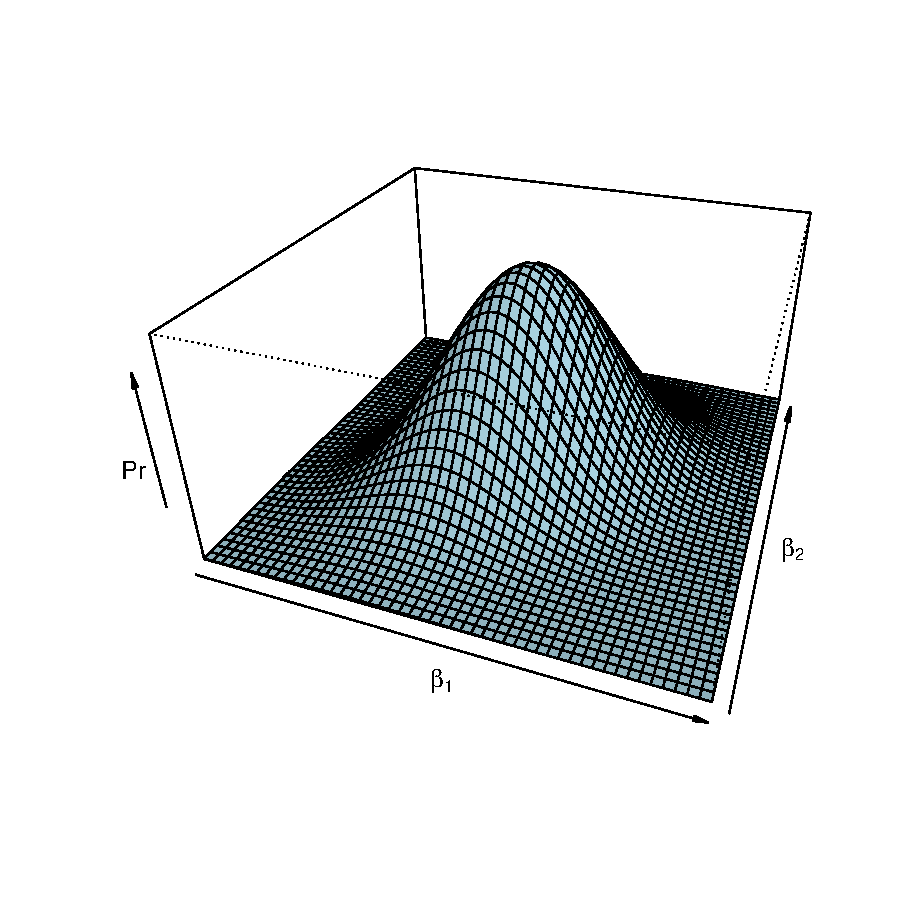
\includegraphics{Tutorial-006}
\end{center}
\caption{Bivariate posterior distribution of $\bm{\beta}$}
\label{densityP}
\end{figure}

For some very simple models the posterior distribution can be derived analytically. Let's imagine that the equation describing the joint posterior distribution of $\beta_{1}$ and $\beta_{2}$ was known and could be plotted (see Figure \ref{densityP}).  The area under the distribution is equal to 1, since we are dealing with a probability, and we can often summarise the posterior distribution using simple statistics.  For example we could state the values of $\beta_{1}$ and $\beta_{2}$ for the peak of the distribution, which would represent the most likely values of $\bm{\beta}$.  We could state the width of the distribution along the $\beta_{1}$ axis as a measure of the precision with which we have estimated $\beta_{1}$, and so on.\\

For most models, however, we cannot derive the posterior distribution analytically, and we must use MCMC to get an approximation.  MCMC relies on the fact that although we cannot derive the complete posterior, we can calculate the height of the posterior distribution at a particular set of co-ordinates. In this example there are only two parameters, so we may be inclined to systematically go through every likely combination of $\beta_{1}$ and $\beta_{2}$ and calculate the height of the distribution at regular distances, and then plot Figure \ref{densityP}.  The Markov chain does exactly this, although it does not move systematically through parameter space (the $\beta_{1}$ and $\beta_{2}$ co-ordinates in this case), it moves stochastically, hence the name 'Monte Carlo'.  There are several ways in which we can get the chain to move in parameter space, and MasterBayes uses a combination of Metropolis-Hastings updates and Gibbs sampling.\\   

\subsection{Metropolis-Hastings Updates and \texttt{tunePed} Objects}

First we need to initialise the chain and specify a set of co-ordinates from which the chain can start a journey through parameter space. Ideally we would like to pick a region of high probability, as we do not want to waste time wandering through regions of low probability: we are not so interested in determining the height of the distribution outside of  Figure \ref{densityP} as it is virtually flat and close to zero (or at least we hope so!).  MasterBayes uses a mixture of Maximum Likelihood and heuristic techniques to detemine the place from which the chain is launched, the co-ordinates of the starting configuration are denoted $\bm{\beta}^{t=0}$.\\

After initialising the chain we need to decide where to go next, and this decision is based on two rules.  First we have to generate a candidate destination, and then we need to decide whether to go there or stay where we are.  There are many ways in which we could generate the candidate coordinates, and MasterBayes uses a well tested and simple method. A random set of cordinates are picked from a multivariate normal distribution that is centered on the initial co-ordinates  $\bm{\beta}^{t=0}$, and has a user specified variance.  We will denote this new set of cordinates as $\bm{\beta}^{new}$. The question then remains whether to move to this new set of cordinates or remain at our current co-ordinates $\bm{\beta}^{t=0} = \bm{\beta}^{old}$.  If the height of the distribution at the new set of co-ordinates is greater, then the chain moves from $\bm{\beta}^{old}$ to $\bm{\beta}^{new}$. If the new set of coordinates is in a region of low probability then the chain may move there, but not all the time.  The probability that the chain moves to low lying areas, is determined by the relative difference bewteen the heights of the posterior distribution at the two co-ordinates.  If the height of the distribution at $\bm{\beta}^{new}$ is 5 times less than the height at $\bm{\beta}^{old}$, then the chain would move to the new set of coordinates 1 in 5 times, and $\bm{\beta}^{t=1}$ would become $\bm{\beta}^{new}$.  Using these rules we can record where the chain has travelled and generate an approximation of the posterior distribution.  Basically, a histogram of Figure \ref{densityP}.\\

The speed with which the chain moves through parameter space is critical, and in part depends on the variance of the proposal distribution.  Say we initialised the chain at the co-ordinates under the peak of the distribution in Figure \ref{densityP}, and specified the variance of the proposal distribution to be large (much larger than the variance of the posterior distribution itself). Many of the candidate co-ordinates would lie outside of Figure \ref{densityP} in regions of very low probability, and since the probability of moving there is low the chain would sit at the peak for large amounts of time.  We would have to run the chain for many iterations before we could generate a histogram that was an adequate approximation of Figure \ref{densityP}.  Alternatively, we could specify the variance to be very small, say a thousand times smaller than the variance of the posterior.  In this case the cordintates $\bm{\beta}^{new}$ and $\bm{\beta}^{old}$ would be very close, and the chain would move almost every iteration since the difference in heights of the posterior at the two cordintates would be tiny.  Although the chain is continuously moving it is travelling such small distances each iteration that the chain would have to pass through many iterations before it adequately covered parameter space.\\  

\texttt{tunePed} objects control the variance of the proposal distributions for parameters updated by Metropolis-Hastings upadtes.  By default, the standard deviation of the proposal distribution will be the standard error of the parameter estimated using Maximum Likelihood.  Scaling constants can then be passed to \texttt{tunePed} which are multiplied by the standard error squared to obtain the variance of the proposal distribution.  Ideally, the chain should move between 20\% and 50\% of the time, and this can be assessed by specifying \texttt{verbose=TRUE} in \texttt{MCMCped}.  The Metroplis-Hastings accpetance rates are then printed to the screen during model fitting.
 
\subsection{Gibbs Sampling}

Gibbs sampling is a special case of Metropolis-Hastings updates, and \texttt{MCMCped} uses Gibbs sampling to sample genotypes and parents.  In the Metropolis-Hastings example above, the Markov Chain was allowed to move in both directions of parameter space simulateously.  An equally valid approach would have been to set up two Metropolis-hastings schemes where the chain was first allowed to move along the $\beta_{1}$ axis, and then along the $\beta_{2}$ axis. In Figure \ref{densityPgibbs} we have cut the posterior distribution of Figure \ref{densityP} in half, and the edge of the surface facing us is the conditional distribution of $\beta_{1}$ given that $\beta_{2}=0$: 

\begin{equation}
Pr(\beta_{1}|\beta_{2}=0, \bm{y}).
\end{equation}

\begin{figure}[!h]
\begin{center}
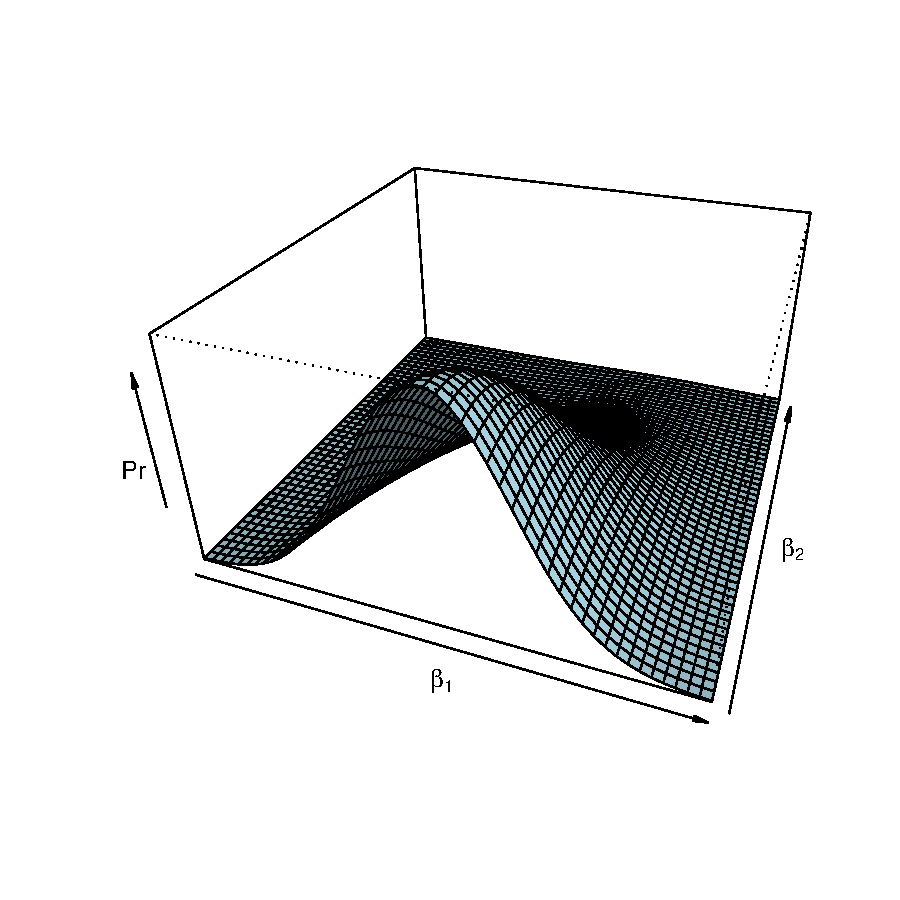
\includegraphics{Tutorial-007}
\end{center}
\caption{Bivariate posterior distribution of $\bm{\beta}$, for postive values of $\beta_{2}$}
\label{densityPgibbs}
\end{figure}

 In some cases, the equation that describes this conditional distribution can be derived despite the equation for the complete joint distribution of Figure \ref{densityP} remaining unknown.  When the conditional distribution of $\beta_{1}$ is known we can use Gibbs sampling. Lets say the chain at a particular iteration is located at zero for $\beta_{2}$.  If we updated $\beta_{1}$ using a Metroplis-Hastings algorithm we would generate a candidate value and evaluate its relative probability compared to the old value.  This procedure would take place in the slice of posterior that is facing us in Figure \ref{densityPgibbs}. However, because we know the actual equation for this slice we can just generate a new value of $\beta_{1}$ directly. This is Gibbs sampling.  If for example, the slice of the posterior that we can see in Figure \ref{densityPgibbs} has a normal distribution with mean of zero and variance of one, then $\beta_{1}^{new}$ can be drawn simply directly from this distribution. This can be much more efficient than Metropolis-Hastings updates, and avoids the issue of having to specigy the variance of a proposal distribution.\\

\subsection{MCMC Diagnostics}
\label{MCMC.D-sec}

When fitting a model using \texttt{MCMCped} the parameter values through which the Markov chain has travelled are stored and returned.  The length of the chain (the number of iterations) can be specified using the \texttt{nitt} argument of \texttt{MCMCped}, and should be long enough so that the posterior approximation is valid.  If we had known the joint posterior distribution in Figure \ref{densityP} we could have set up a Markov chain that sampled directly from the posterior.  If this had been the case each successive value in the Markov chain would be independent of the previous value after conditioning on the data, ${\bm y}$, and a thousand iterations of the chain would have produced a histogram that resembled Figure \ref{densityP} very closely.  However, generally we do not know the joint posterior distribution of the parameters, and we use Gibbs sampling and Metropolis-Hastings updates to approximate this distribution. For this reason the parameter values of the Markov chain at sucessive iterations are usually not idependent and care needs to be taken regarding the validity of the approximation.  \texttt{MCMCped} returns the Markov chain for continous parameters as \texttt{mcmc} objects, which can be analysed using the \texttt{coda} pacakge.  The function \texttt{autocorr} estimates the level of non-independence between succesive samples in the chain\footnote{Later versions of MasterBayes $>$2.2 also include the function \texttt{autocorrP} which calculates an autocorrelation metric for parentage assignements when \texttt{write\_postP="JOINT"} is sepcified in \texttt{MCMCped}.}.  When autocorrelation is high the chain needs to be run for longer, and this can lead to storage problems for high dimensional problems. The argument \texttt{thin} can be passed to \texttt{MCMCped} specifying the intervals at which the Markov chain is stored.\\

The approximation obtained from the Markov chain is conditional on the set of parameter values that were used to initialise the chain.  In many cases the first iterations show a strong dependence on the starting parameteristaion, but as the chain progresses this dependence may be lost.  As the dependence on the starting parameterisation diminishes the chain is said to converge and the argument \texttt{burnin} can be passed to \texttt{MCMCped} specifying the number of iterations which must pass before samples are stored.  Assessing convergence of the chain is notoriously difficult.  The posterior distribution in Figure \ref{densityP} has a simple form and the convergence of the chain would be easy to acheive.  If however, the posterior was multimodal convergence would be harder to acheive and diagnose.\\  
 


\begin{figure}[!h]
\begin{center}
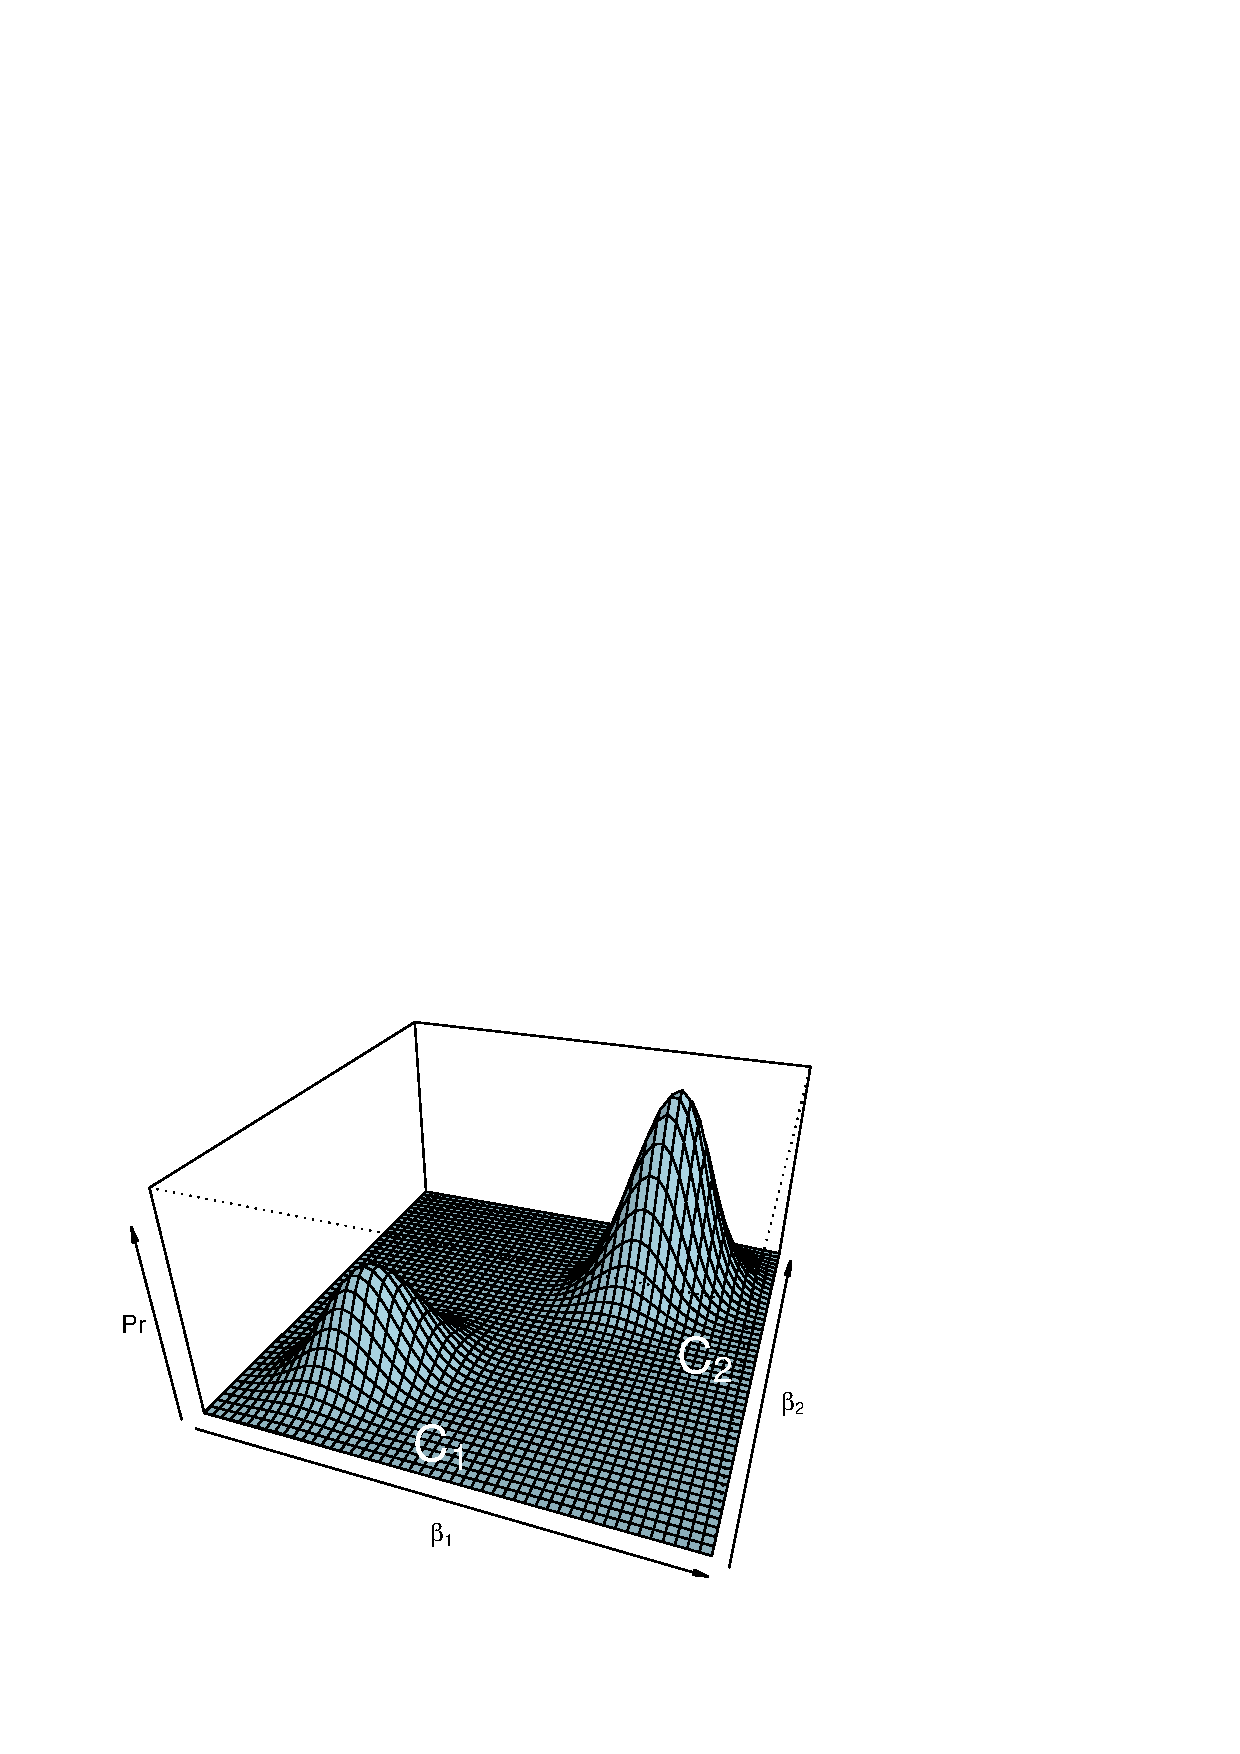
\includegraphics{Tutorial-008}
\end{center}
\caption{A bimodal bivariate posterior distribution of $\bm{\beta}$.}
\label{densityPMM}
\end{figure}

For example, imagine a chain was initailised at $\textrm{C}_{1}$ in Figure \ref{densityPMM}. The chain may provide valid approximates for the region of high probablity at small values of $\beta_{1}$ and $\beta_{2}$ but it may 
fail to pass under the low probability ridge that connects the two high probability regions.  Conclusions drawn from a chain initialised a $\textrm{C}_{2}$ may be very different, and it is good practice to run multiple chains from different starting parametrisations (See Section \ref{SHC} for an interesting example).  For \texttt{MCMCped} models in which the posterior distribution of genotypes is estimated, it is particularly important to assess the sensitivity of the chain to different starting configurations.  Genotype configurations with high probability may be separated by configurations of low probability and the chain may mix poorly.  See Section \ref{Error-sec} for an example where high probability genotype configurations are actually separated by configurations of zero probability.  In such cases the chain is said to be reducible and posterior simulation is not possible.

\subsection{Prior Specifications and \texttt{priorPed} Objects}
\label{prior-sec}

The posterior distribution is the product of the likelihood and the prior. If a prior is not specified using the function \texttt{priorPed}, the default is to use an improper uniform prior for all parameters, except allele frequencies, which have a vague Dirichlet prior. For the size of the unsampled population and the genotyping error rates the prior has zero probability for negative values.  When the posterior distribution itself is improper (i.e if the volume under the surfaces plotted in Figures \ref{densityP} and \ref{densityPMM} are not finite) then the posterior can no longer be treated as a probability, and inferences taken from it would be compromised.  For some models the data will contain enough information to make the posterior proper despite an improper prior specification. However, for chains in which a sampled pedigree has little or no structure (i.e. all parents are unsampled), or no sampled parents exist for some level of a categorical predictor variable\footnote{It turns out that this is a common problem in real datasets and has been refered to as the extreme category problem.  For example, the catgorical variable \texttt{`recorded in that year/only recorded in the previous year'} may be fitted to account for individuals that were not recorded but may have been alive.  If these indiviuals really were dead then the estimated probability of them having offspring tends to zero which is $-\infty$ on the logit scale.  This problem can usually be idenitified by the chain making long excursions into extreme values of the parameter space.}, then problems can occur unless informative priors are used. In the extreme case, models in which parameters are confounded, a proper prior distribution is required to make the parameters idenitifiable.  Imagine that all territorial males were old, and all non-territorial males were young. If we tried to fit the two parameters, $\beta_{1}$ and $\beta_{2}$, in a single model we would run in to difficulties.  The parameters are not identifiable because we cannot distinguish between the two alternatives; whether territorial males gain more paternity beacuse they hold a territory, or because they are older.  The likelihood surface for $\bm{\beta}$ would look something like Figure \ref{likP}, with a ridge of high probability extending to infinity.\\  

\begin{figure}[!h]
\begin{center}
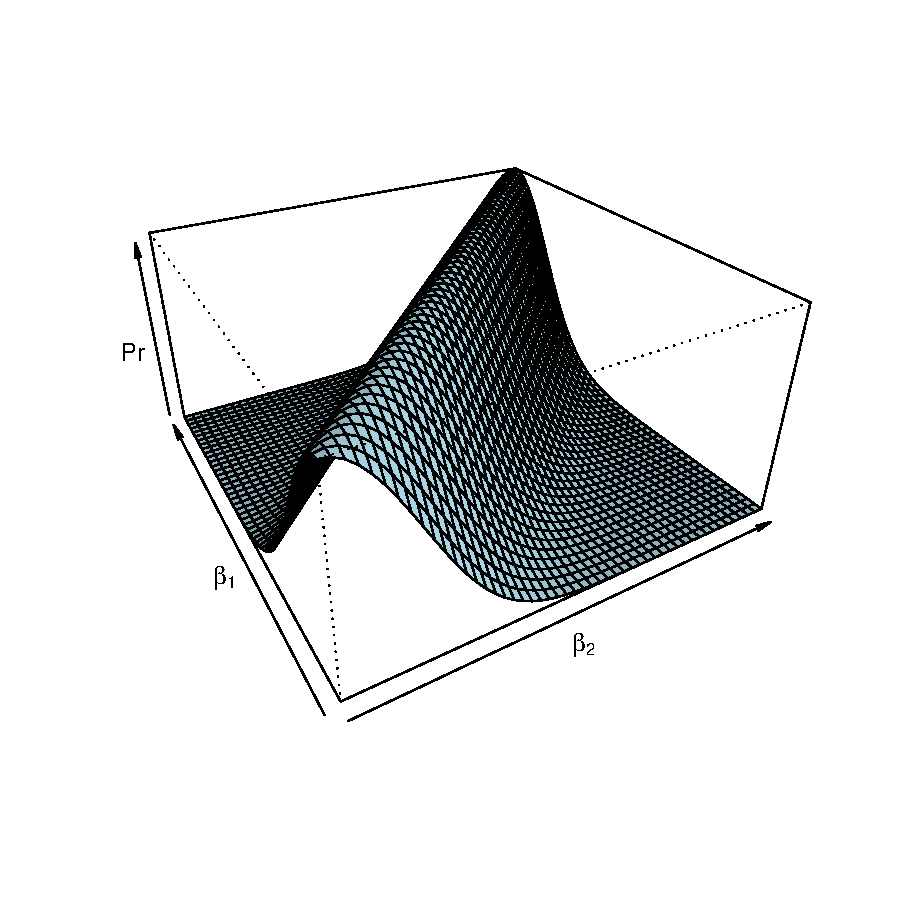
\includegraphics{Tutorial-009}
\end{center}
\caption{The likelihood of $\bm{\beta}$, when the two parameters are not identifiable from the data, $\bm{y}$}
\label{likP}
\end{figure}

In this insatnce the Markov chain would wander aimlessly along the ridge, perhaps even giving the appearance of having converged.  MasterBayes will not check whether all parameters are idenitifiable.

\section{\large{A Worked Example: The Seychelles Warbler}}
\label{Warbler-sec}

To illustrate the basic methodology, I will use data collected in 1999 from the Cousin Island population of the endangered Seychelles warbler \citep{Richardson.2001}. 

\begin{Schunk}
\begin{Sinput}
> data(WarblerP)
> data(WarblerG)
\end{Sinput}
\end{Schunk}

 \texttt{WarblerP} is a data frame containing phenotypic data for all individuals recorded in that year.  This includes a unique identifier for each bird, its sex and the territory it was recorded on. \texttt{offspring} is a binary vector with 1 indicdating the bird was born in 1999, and \texttt{status} is a factorial vector with 2 levels indidcating whether the bird is a dominant or a subordinate. \texttt{lat} and \texttt{long} are x and y coordinates for the centre of each bird's territory. {WarblerG} is a data frame containing the genotypes of each individual at 14 loci \citep{Richardson.2000}.\\

In this particular year there were 59 offspring, 127 adult females and 121 adult males recorded on the island.  We will assume for now that an offspring's mother is always found on the same territory as the offspring, but that an offspring's father could potentially be any one of the 121 sampled males, or even a male that was not sampled.  Initially, we will focus on modelling the degree to which offspring and fathers are associated spatially, by estimating the rate at which the probability of paternity drops with distance from the offspring.  This rate ($\beta$) is the exponential rate parameter, and we are interested in its probability distribution given the data we have collected:


\begin{equation}
Pr(\beta | \bm{G}_{obs}, \textrm{\texttt{lat}}, \textrm{\texttt{long}}, \textrm{\texttt{terr}}).
\label{no_pedigree-eq}
\end{equation}

$\bm{G}$ represents genotypes, and we use the subscript $_{obs}$ to indicate observed rather than actual genotypes. This distinction is necessary when genotyping error is present (see Section \ref{GE-sec}).  Evaluating the problem in this form is intractable, but the problem can be simplified by augmenting with the pedigree, $\bm{P}$:

\begin{equation}
\int_{\bm P}Pr(\beta,  {\bm P}| \bm{G}_{obs}, \textrm{\texttt{lat}}, \textrm{\texttt{long}}, \textrm{\texttt{terr}})d{\bm P}.
\label{pedigree-eq}
\end{equation}

Equations \ref{no_pedigree-eq} and \ref{pedigree-eq} are equivalent. In the latter case we estimate the pedigree, but we also integerate over any uncertainity that may remain regarding its structure, leaving us with the marginal distribution of $\beta$.  We will start by fitting commonly used approximations to equation \ref{pedigree-eq} and end by a fitting a model that is very close to being exact.

\subsection{Phenotypic Predictors}
\label{pred-sec}

 To fit the model we need to start by creating a variable that indicates whether particular females and particular offspring occur on the same territory.  Unfortunately the nature of these models precludes us from using the R formula mini-language,  and so variables are created using \texttt{varPed} and then evaluted as part of the model formula in a \texttt{PdataPed} object

\begin{Schunk}
\begin{Sinput}
> res1 <- expression(varPed(x = "terr", gender = "Female", relational = "OFFSPRING", 
+     restrict = "=="))
\end{Sinput}
\end{Schunk}

\texttt{x} is the variable we are interested in, in this case territories.  \texttt{gender} specifies whether the variable relates to maternity (\texttt{gender="Female"}), paternity (\texttt{gender="Male"}) or both (\texttt{gender=NULL}). The argument \texttt{relational} is a little more complex, and sepcifies whether the variable is to be treated as it is (\texttt{relational=FALSE}), or is to be transformed into a distance.  \texttt{relational="OFFSPRING"} creates a variable that is the distance between \texttt{x} measured in the offspring and the parent, and \texttt{relational="MATE"} is the distance between \texttt{x} measured in a potential mother and a potential father.  When \texttt{x} is numeric, the transformed variable is a Euclidean distance \footnote{Later versions of MasterBayes ($>2.1$) also include the options \texttt{relational="OFFSPRINGV"} and \texttt{relational="MATEV"} which create a vector of the difference between the two phenotypes (but not absoluted). i.e $x=x_{i}-x_{j}$ rather than $x=\sqrt{x^{2}_{i}-x^{2}_{j}}$.}. When \texttt{x} is a factor, the transformed variable is a logical vector with \texttt{TRUE} indicating that \texttt{x} for the two indivdiuals are the same, and \texttt{FALSE} indicating that they are different.  In this example we are dealing with a logical variable that is \texttt{TRUE} when offspring and females are present on the same territory, and \texttt{FALSE} if not. We could estimate a parameter associated with this variable which would be interpreted as the probability of within territory maternity.  However, in this case we are assuming that extra territory maternity does not occur and we can use the argument \texttt{restrict="=="} to retain mothers that have the same territory as the offspring for the transformed variable. Females that are on a different territory to the offspring are excluded as mothers. This is essentially a strong prior on the parameter associated with within territory/extra territory maternity, but is computationaly faster because excluded mothers can be discarded for particular offspring.\\

We also need to exclude indidvuals that are born in 1999 as potential parents
 
\begin{Schunk}
\begin{Sinput}
> res2 <- expression(varPed(x = "offspring", gender = NULL, relational = FALSE, 
+     restrict = 0))
\end{Sinput}
\end{Schunk}

We want to exclude individuals that have 1 in the variable \texttt{offspring}, as they represent chicks born in 1999.  We want to exclude offspring irrelevant of their sex so  \texttt{gender=NULL}  and we want to evaluate \texttt{x} as it is (i.e. as a binary variable).  We exclude offspring by specifying \texttt{restrict=0} which retains individuals that have 0 in the offspring variable.\\

The goal of the analysis is to estimate $\beta$, the rate at which paternity drops with distance from an offspring

\begin{Schunk}
\begin{Sinput}
> var1 <- expression(varPed(x = c("lat", "long"), gender = "Male", 
+     relational = "OFFSPRING"))
\end{Sinput}
\end{Schunk}

\texttt{x} in this instance contains two variables that specify the cordinates of each indivdual on the island. Because \texttt{relational="OFFSPRING"} this variable is interpreted as the Euclidean distance between offspring and fathers (\texttt{gender="Male"}) in 2 dimensions.  \texttt{restrict} is not specified indicdiating that all males are potential fathers. 

\begin{equation}
p^{(o)}_{i,j} \propto \textrm{exp}(\beta \sqrt{(\textrm{\texttt{lat}}_{j}-\textrm{\texttt{lat}}_{o})^{2}+(\textrm{\texttt{long}}_{j}-\textrm{\texttt{long}}_{o})^{2}})
\label{dist-eq}
\end{equation}

The full notation for a multinomial model is cumbersome so I'll express all models in this form for clarity. A full list of models and the associated \texttt{varPed} specificiations can be found in Appendix \ref{models-app}. $p^{(o)}_{i,j}$ is the probability that female $i$ and male $j$ are the parents of offspring $o$.\\  

 These variables are to be evaluated inside various functions, and they need to be associated with the \texttt{data.frame} in which \texttt{x} is stored. We also need to provide data on the sex, age, and id of each individual.  This is done by creating a \texttt{PdataPed} object.

\begin{Schunk}
\begin{Sinput}
> PdP <- PdataPed(formula = list(res1, res2, var1), data = WarblerP, 
+     USsire = TRUE)
\end{Sinput}
\end{Schunk}

The variables are passed as a list to the argument \texttt{formula}, and the relevant data are contained in \texttt{WarblerP}.  In this case variables named \texttt{id}, \texttt{sex} and \texttt{offspring} exist in \texttt{WarblerP} and they do not need to be specified explicitly.  All \texttt{PdataPed} objects must contain an \texttt{id} and \texttt{offspring} variable containing unique identifiers for each individual, and a vetcor indicdating whether records belong to offspring. If \texttt{data} does not have a sex column, or \texttt{sex=NULL}, the data are assumed to have been collected from a hermaphrodite system (see Sections \ref{Herm-sec} and \ref{SHC}). Elements of the sex vector must be either \texttt{"Male"}, \texttt{"Female"} or \texttt{NA}.  In this model we also allow for the presence of unsampled males: \texttt{USsire=TRUE}.\\

We also need to create a \texttt{GdataPed} object for storing the genotype data and some associated information

\begin{Schunk}
\begin{Sinput}
> GdP <- GdataPed(G = WarblerG, categories = NULL)
\end{Sinput}
\end{Schunk}

\texttt{GdataPed} objects store genotype data (\texttt{G}) as a list of \texttt{genotype} objects for dominant markers (see the package genetics), or \texttt{genotypeD} objects for dominant markers.  A list of \texttt{genotype} or \texttt{genotypeD} objects can be directly passed to the argument \texttt{G}, or a data frame can be passed that is coerced to a list of genotype objects using the function \texttt{genotype.list}. The variable \texttt{id} is required, and links genotypes with individuals.  Indivdiuals can have multiple genotypes if they have been genotyped more than once.  If \texttt{G} is a data.frame with a column named \texttt{id}, \texttt{id} does not have to be explicitly passed to \texttt{GdataPed}.  If \texttt{categories} is not specified then genotyping error rates are assumed not to vary across genotypes, otherwise \texttt{categories} must be a vector of factors the same length as \texttt{id}.\\

\subsection{Approximate Methods and \texttt{startPed} Objects}
\label{approx-sec}

The optional \texttt{startPed} object specifies the starting parameterisation for the model, and logical arguments specifying which parts of the model are to be fixed at the starting parameterisation and not to be estimated. Maximum likelihood or heuristic starting parameterisations are used by default, and all estimable parameters are estimated, unless ortherwise specified. These parameters may include the pedigree (\texttt{P}), genotypes (\texttt{G}), base population allele frequencies (\texttt{A}), allelic dropout rates \texttt(E1), stochastic genotping error rates (\texttt {E2}), unsampled male (\texttt{USsire}) and female (\texttt{USdam}) population sizes\footnote{In later versions of MasterBayes (>2.1) male and female unsmapled population sizes can be forced to be equal by specifying \texttt{estUSsire="USdam"} in the \texttt{startPed} object.}, and most importantly the parameters of the multinomial log-linear model (\texttt{beta}). Estimating all unknown parameters can be computationaly intensive, and preliminary analyses can usually be caried out using approximate methods.  A commonly used approximation for dealing with genotyping error is to integrate out any uncertainty prior to the parentage anlaysis (See Section \ref{Error-sec}).  We can use the approximation by specifying \texttt{estG=FALSE}; if we were to use the exact solution we would be required to estimate the actual genotypes of all individuals.  When \texttt{estG=FALSE}, error rates and allele frequencies are also unestimable and need to be specified.  If the approximation is used, the corrected model of genotyping error used by CERVUS is implemented \citep{Kalinowski.2006}, and \texttt{E2} is the per-allele probability of an error.  In CERVUS this is specified as a per-genotype probaility, and the default value of 0.005 is close to the CERVUS default ($0.01 \approx 2(1-0.005)0.005+0.005^{2}$).  Allele frequencies, if not specified, are taken directly from the genotype data using the function \texttt{extractA}.  


\subsection{Categorical Estimation}
\label{cat-sec}

The most popular software for parentage anlaysis is CERVUS \citep{Marshall.1998}.  MasterBayes can fit CERVUS type models as a special case, although two major differences exist between the MasterBayes implementation and the CERVUS implementation.  Firstly,  mothers and fathers can be estimated simultaneously in MasterBayes, whereas CERVUS was developed for systems where one parent is already known\footnote{Joint estimation of maternity and paternity is now available in version 3 of CERVUS.}.  Secondly, in MasterBayes confidence in parentage assignments is assesed at the level of individual assignments and the measure of confidence uses all the information provided by potential parents.  CERVUS on the otherhand assesses confidence at the level of the population, and only uses the information provided by the two most likely parents \citep{Nielsen.2001}. By default, the model defined in Equation \ref{pedigree-eq} is fitted with the minimal amount of approximation.  To fit a CERVUS type approximation we need to do a little more work.  We need to specify that an approximation is to be used for genotyping error, and we need to provide point estimates for the allele frequencies and the genotyping error rate (see Sections \ref{approx-sec} and \ref{GE-sec}).  We also need to specify that the number of unsampled males is not to be estimated (see Section \ref{us-sec}), and that a point estimate of 10 is to be used instead. 

\begin{Schunk}
\begin{Sinput}
> sP <- startPed(estG = FALSE, E2 = 0.005, A = extractA(WarblerG), 
+     estUSsire = FALSE, USsire = 10)
\end{Sinput}
\end{Schunk}


CERVUS breaks the problem down into two stages.  In the fisrt stage the pedigree is estimated using the genetic data alone, and this pedigree (or part of it) is then passed to the second stage, where the spatial parameter, $\beta$ is estimated.  We start by estimating the pedigree using the function \texttt{MCMCped} which returns samples of the posterior distribution of all unkowns.

\begin{Schunk}
\begin{Sinput}
> PdPCervus <- PdataPed(formula = list(res1, res2), data = WarblerP, 
+     USsire = TRUE)
> model1 <- MCMCped(PdP = PdPCervus, GdP = GdP, sP = sP, verbose = FALSE)
\end{Sinput}
\begin{Soutput}
[1] "using an approximation for genotyping error"
\end{Soutput}
\end{Schunk}

Note that we have created a new \texttt{PdataPed} object, \texttt{PdPCervus}, that does not contain the distance variable as we wish to use the genetic data only to infer parentage.  Beacuse the only unkown in this model is the pedigree the object \texttt{model1} only contains a single element (\texttt{P}): the posterior distribution of the pedigree.  By default this is the marginal distribution of parental pairs, and we can extract the mode of this distribution

\begin{Schunk}
\begin{Sinput}
> ped1 <- modeP(model1$P, threshold = 0)
> ped1[1:10, ]
\end{Sinput}
\begin{Soutput}
      [,1]      [,2]      [,3]     
 [1,] "N748835" "K278102" "USsire" 
 [2,] "Z993558" "K278102" "K278027"
 [3,] "N748825" "K278115" "N021716"
 [4,] "N748841" "N021991" "K278027"
 [5,] "N748842" "J368410" "USsire" 
 [6,] "N748848" "J854303" "K278101"
 [7,] "Z993553" "K278011" "J368403"
 [8,] "N748838" "N021965" "N021760"
 [9,] "N748827" "K278018" "N021839"
[10,] "Z993562" "K278018" "USsire" 
\end{Soutput}
\end{Schunk}

In this example the most likely pedigree for the first ten offspring is displayed, with the offspring, dam and sire in each column.  If the most likely father for one of these offspring is unsampled then the respective element of the sire column is designated as \texttt{USsire}. For such a simple model, Markov chain Monte Carlo is redundant as the posterior distribution of the pedigree can be calculated analyticly

\begin{Schunk}
\begin{Sinput}
> ped2 <- MLE.ped(getXlist(PdPCervus, GdP), USsire = TRUE, nUSsire = 10)
> ped2[3:12, ]
\end{Sinput}
\begin{Soutput}
      [,1]      [,2]      [,3]     
 [1,] "N748835" "K278102" NA       
 [2,] "Z993558" "K278102" "K278112"
 [3,] "N748825" "K278115" "N021716"
 [4,] "N748841" "N021991" "K278027"
 [5,] "N748842" "J368410" NA       
 [6,] "N748848" "J854303" "K278101"
 [7,] "Z993553" "K278011" "J368403"
 [8,] "N748838" "N021965" "N021760"
 [9,] "N748827" "K278018" "N021839"
[10,] "Z993562" "K278018" NA       
\end{Soutput}
\end{Schunk}

This is the Maximum Likelihood estimate of ${\bm P}$ and is equivalent, in this model, to the Bayesian estimate when all parental combinations have an equal prior probability of being the parents.  We will return to the function \texttt{getXlist} later, and proceed to estimate $\beta$ assuming the MLE/posterior mode of the pedigree is the true pedigree.  We do this by passing the ML pedigree (\texttt{dam=ped2[,2]} and \texttt{sire=ped2[,3]}) to a \texttt{startPed} object, and by specifying that the pedigree should not be estimated (\texttt{estP=FALSE}), but should be fixed.

\begin{Schunk}
\begin{Sinput}
> sP <- startPed(estP = FALSE, dam = ped2[, 2], sire = ped2[, 3], 
+     estUSsire = FALSE)
> model2 <- MCMCped(PdP = PdP, sP = sP, verbose = FALSE)
> plot(model2$beta)
> summary(model2$beta)
\end{Sinput}
\begin{Soutput}
Iterations = 1:1000
Thinning interval = 1 
Number of chains = 1 
Sample size per chain = 1000 

1. Empirical mean and standard deviation for each variable,
   plus standard error of the mean:

          Mean             SD       Naive SE Time-series SE 
    -0.0705708      0.0095894      0.0003032      0.0002839 

2. Quantiles for each variable:

    2.5%      25%      50%      75%    97.5% 
-0.08912 -0.07720 -0.07046 -0.06364 -0.05249 
\end{Soutput}
\end{Schunk}



\begin{figure}[!h]
\begin{center}
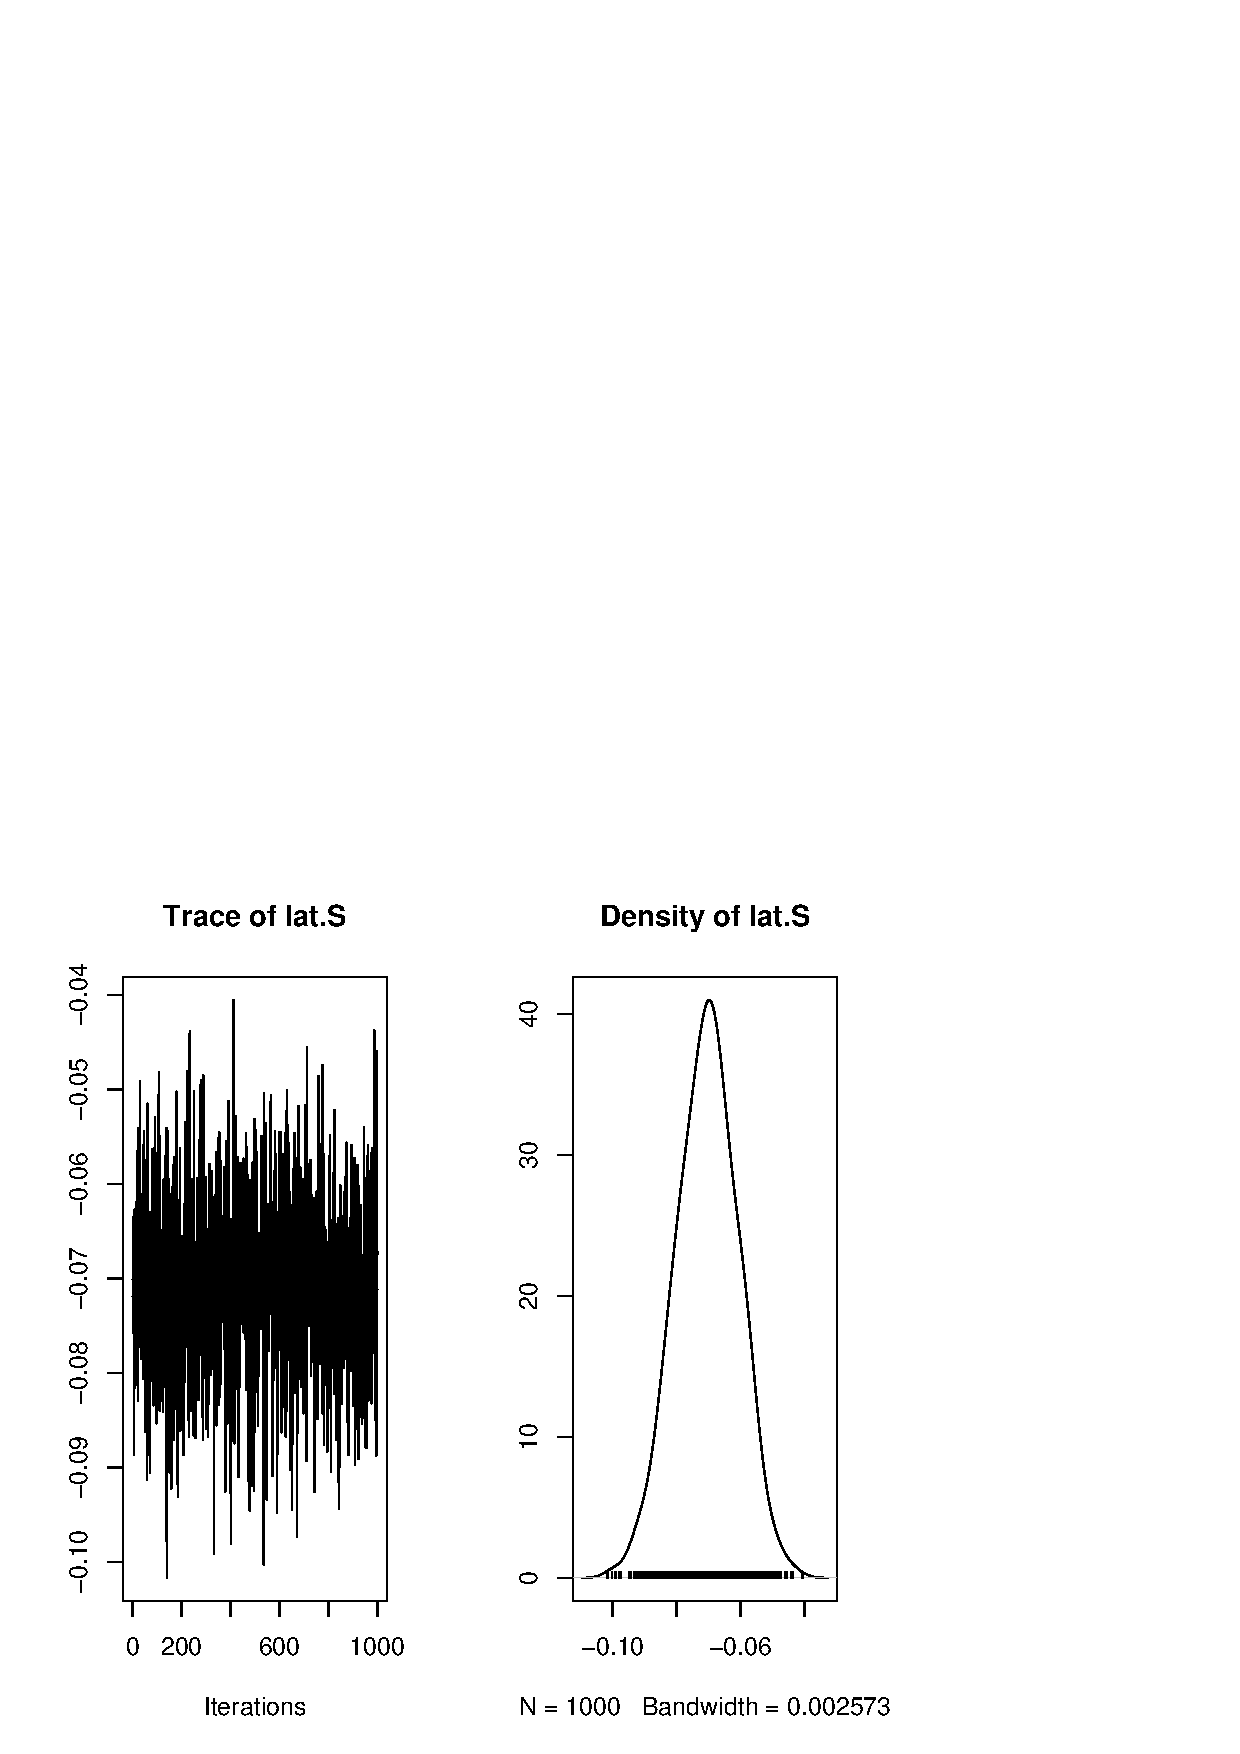
\includegraphics{Tutorial-022}
\end{center}
\caption{Posterior distribution of $\bm{\beta}$ from \texttt{model2}. The posterior is conditional on the categorical assignment of the pedigree being true. These plots are a way of summarising a Markov Chain using the coda package.  The left plot is a trace of the sampled posterior, and can be thought of as a time series.  The right plot is a density estimate, and can be thought of a smoothed histogram approximating the posterior.  See Section \ref{MCMC-sec} for more details.}
\label{model2beta}
\end{figure}

The genetic data are not required since the pedigree is treated as known, and only the \texttt{PdataPed} object (\texttt{PdP}) needs to be passed to \texttt{MCMCped}.  Again, with such a simple model, Maximum Likelihood gives valid results, and the large sample approximation for the standard error is close to the Bayesian estimate. 


\begin{Schunk}
\begin{Sinput}
> MLElat <- MLE.beta(getXlist(PdP), ped2)
> MLElat$beta
\end{Sinput}
\begin{Soutput}
            [,1]
[1,] -0.06987857
\end{Soutput}
\begin{Sinput}
> sqrt(MLElat$C)
\end{Sinput}
\begin{Soutput}
            [,1]
[1,] 0.009572814
\end{Soutput}
\end{Schunk}


Despite the two methods giving similar estimates, they are both severely biased towards zero; the value of $\beta$ that would be observed if fathers were distributed randomly across the island with respect to their offspring.  We can get a feel for this by estimating $\beta$ for those paternity assignments that had a probability exceeding 0.9.   

\begin{Schunk}
\begin{Sinput}
> ped3 <- modeP(model1$P, threshold = 0.9)
> ped3[1:10, ]
\end{Sinput}
\begin{Soutput}
      [,1]      [,2]      [,3]     
 [1,] "N748835" "K278102" NA       
 [2,] "Z993558" "K278102" NA       
 [3,] "N748825" "K278115" NA       
 [4,] "N748841" "N021991" NA       
 [5,] "N748842" "J368410" NA       
 [6,] "N748848" "J854303" "K278101"
 [7,] "Z993553" "K278011" "J368403"
 [8,] "N748838" "N021965" "N021760"
 [9,] "N748827" "K278018" NA       
[10,] "Z993562" "K278018" NA       
\end{Soutput}
\begin{Sinput}
> MLElat3 <- MLE.beta(getXlist(PdP), ped3)
> MLElat3$beta
\end{Sinput}
\begin{Soutput}
           [,1]
[1,] -0.2965067
\end{Soutput}
\begin{Sinput}
> sqrt(MLElat3$C)
\end{Sinput}
\begin{Soutput}
          [,1]
[1,] 0.0517371
\end{Soutput}
\end{Schunk}

The first thing to notice is that by only using males that have a greater than 0.9 probability of being the father, we are excluding 75\% of the offspring from the analysis. Because of this the standard error of $\beta$ is more than 5 times larger than that in the previous model.  However, the ML estimate of $\beta$ is significantly larger than in the previous model suggesting that our basic model is wrong. 


\subsection{Full Probability Estimation}
\label{fp-sec}

 The reason that it is wrong is beacuse we have failed to use the information contained in the phenotypic data to help us estimate the pedigree.  Equation \ref{pedigree-eq} can be rewritten

\begin{equation}
\frac{Pr(\beta,  {\bm P}| {\bm G}_{obs}, \textrm{\texttt{lat}}, \textrm{\texttt{long}}, \textrm{\texttt{terr}})}{Pr({\bm P}| \beta {\bm G}_{obs}, \textrm{\texttt{lat}}, \textrm{\texttt{long}}, \textrm{\texttt{terr}})}.
\label{pedigree_expanded}
\end{equation}

and can be simplified  under the assumption that the genetic data provide no information regarding $\beta$ once the pedigree is known

\begin{equation}
\frac{Pr({\bm G}_{obs} | {\bm P})Pr({\bm P} | \beta,\textrm{\texttt{lat}}, \textrm{\texttt{long}}, \textrm{\texttt{terr}})}{Pr({\bm P}| \beta, {\bm G}_{obs}, \textrm{\texttt{lat}}, \textrm{\texttt{long}}, \textrm{\texttt{terr}})}Pr({\bm P}, \beta)
\label{pedigree_simplifies}
\end{equation}

The fundamental difference between the exact solution implemented in MasterBayes and the approximations used in categorical and fractional type approaches lies in the denominator of equation \ref{pedigree_simplifies}.  This equation highlights the importance of using the phenotypic data to aid pedigree reconstruction, and the central role that $\beta$ plays in mediating this information.  The CERVUS type approximation makes the mistake of assuming that only the genetic data are required to estimate the pedigree \citep[see the information boxes in][]{Hadfield.2006c}.\\

  We can fit a model where the pedigree and $\beta$ are estimated simultanously, although for now we will retain the CERVUS type approximation for genotyping error and the number of unsampled males.

\begin{Schunk}
\begin{Sinput}
> sP <- startPed(estG = FALSE, A = extractA(WarblerG), E2 = 0.005, 
+     estUSsire = FALSE, USsire = 10)
> model3 <- MCMCped(PdP = PdP, GdP = GdP, sP = sP, verbose = FALSE)
\end{Sinput}
\begin{Soutput}
[1] "using an approximation for genotyping error"
\end{Soutput}
\begin{Sinput}
> plot(model3$beta)
> summary(model3$beta)
\end{Sinput}
\begin{Soutput}
Iterations = 1:1000
Thinning interval = 1 
Number of chains = 1 
Sample size per chain = 1000 

1. Empirical mean and standard deviation for each variable,
   plus standard error of the mean:

          Mean             SD       Naive SE Time-series SE 
    -0.2548820      0.0309223      0.0009778      0.0015165 

2. Quantiles for each variable:

   2.5%     25%     50%     75%   97.5% 
-0.3190 -0.2736 -0.2534 -0.2336 -0.1978 
\end{Soutput}
\end{Schunk}
 


\begin{figure}[!h]
\begin{center}
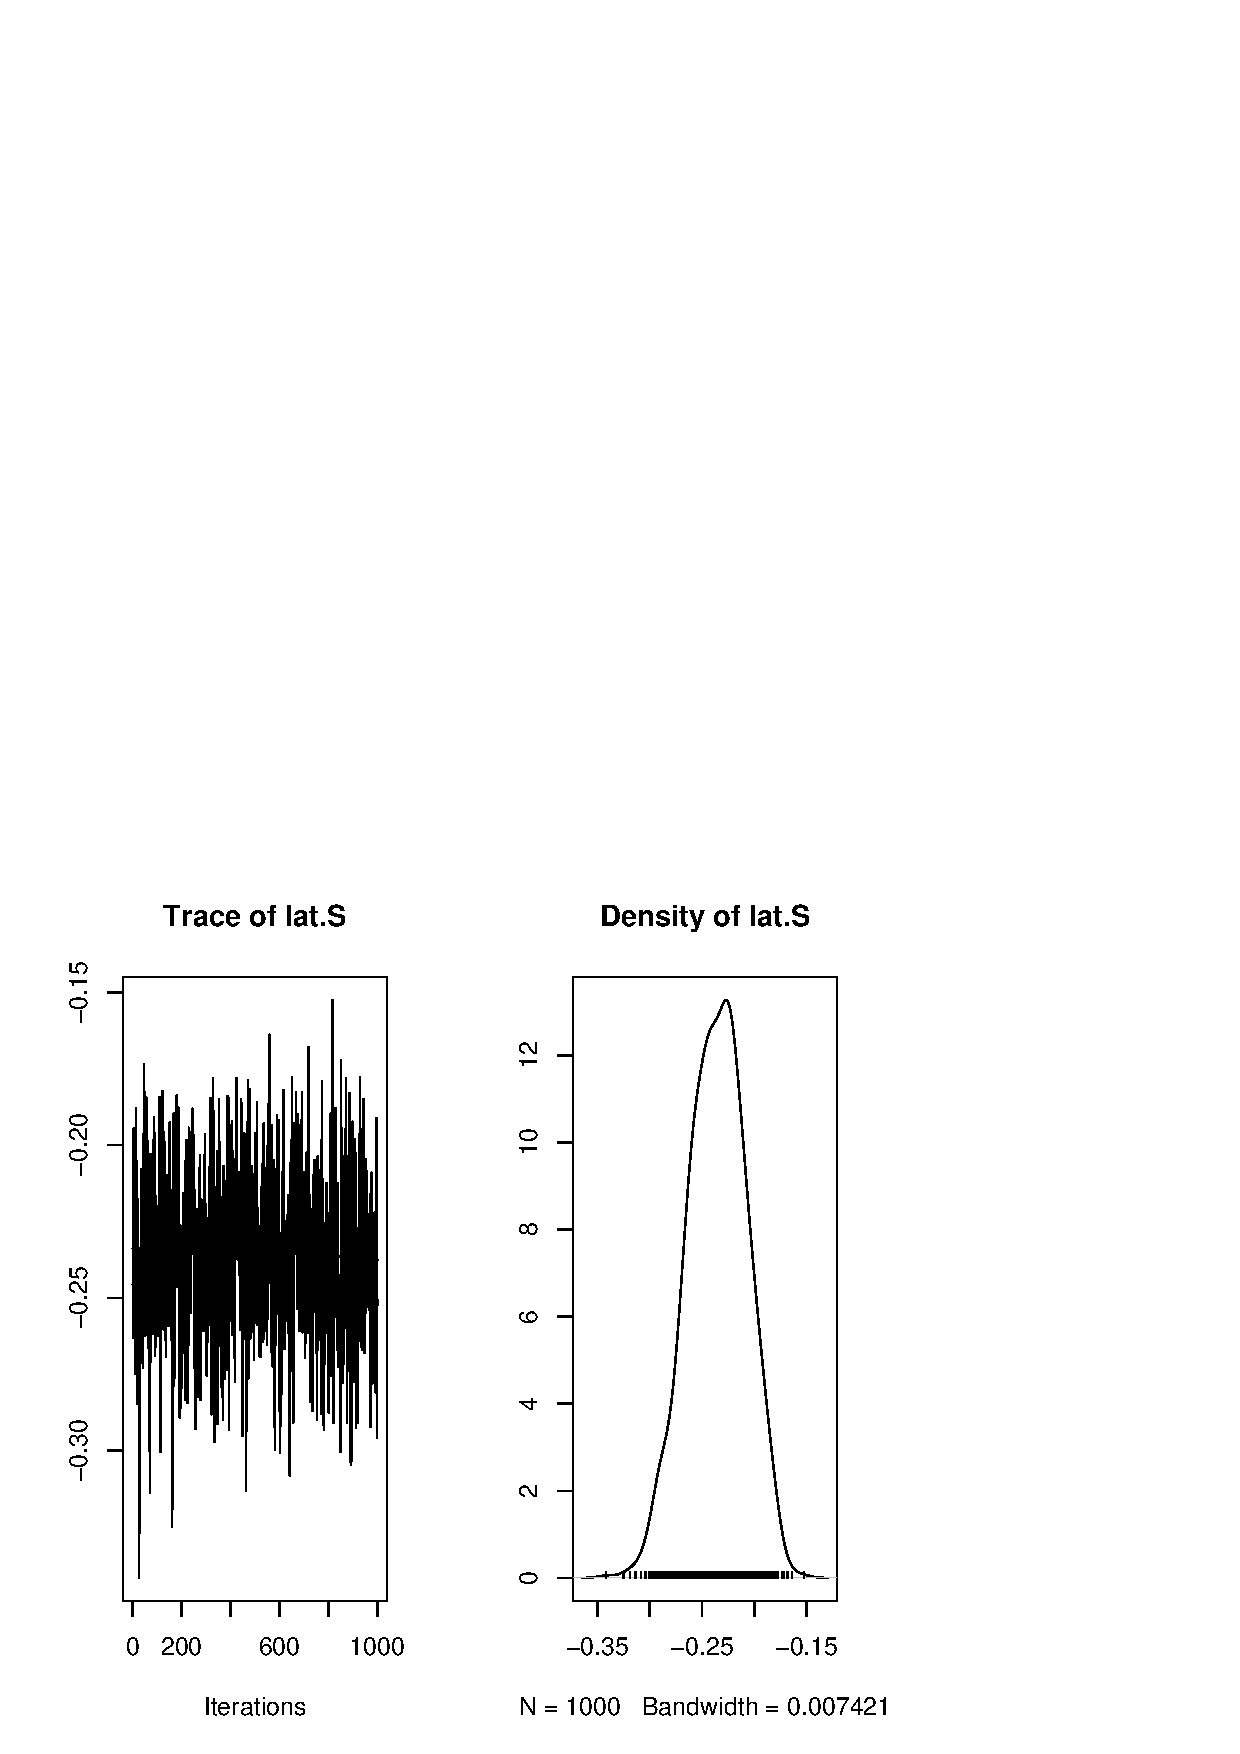
\includegraphics{Tutorial-027}
\end{center}
\caption{Posterior distribution of $\bm{\beta}$ from \texttt{model3}. The pedigree and $\beta$ have been simultaneously estimated, but an approximation for genotyping error has still been used. It was also assumed that the we size of the unsampled population and the genotyping error rate were known.}
\label{model3beta-fig}
\end{figure}


This estimate is much closer to the ML estimate for the restricted pedigree \texttt{ped3}, although the standard error is tighter because the whole pedigree is used.  It should also be noted that the ML standard error is artificially low because it does not take into account the uncertainty in the pedigree.  This is another draw back of the categorical approach; once the pedigree is estimated you then have to treat it as if it was known with complete certainity, rather than a random variable. \\

\subsection{Unsampled Parents}
\label{us-sec}

Next we will relax the assumption that the number of unsampled males is 10 and simultaneously estimate the number from the data:

\begin{Schunk}
\begin{Sinput}
> sP <- startPed(estG = FALSE, A = extractA(WarblerG), E2 = 0.005)
> model4 <- MCMCped(PdP = PdP, GdP = GdP, sP = sP, verbose = FALSE)
\end{Sinput}
\begin{Soutput}
[1] "using an approximation for genotyping error"
\end{Soutput}
\begin{Sinput}
> plot(model4$USsire)
> summary(model4$USsire)
\end{Sinput}
\begin{Soutput}
Iterations = 1:1000
Thinning interval = 1 
Number of chains = 1 
Sample size per chain = 1000 

1. Empirical mean and standard deviation for each variable,
   plus standard error of the mean:

          Mean             SD       Naive SE Time-series SE 
       35.9265        15.0032         0.4744         0.5258 

2. Quantiles for each variable:

 2.5%   25%   50%   75% 97.5% 
13.39 25.56 33.79 43.99 71.92 
\end{Soutput}
\end{Schunk}


\begin{figure}[!h]
\begin{center}
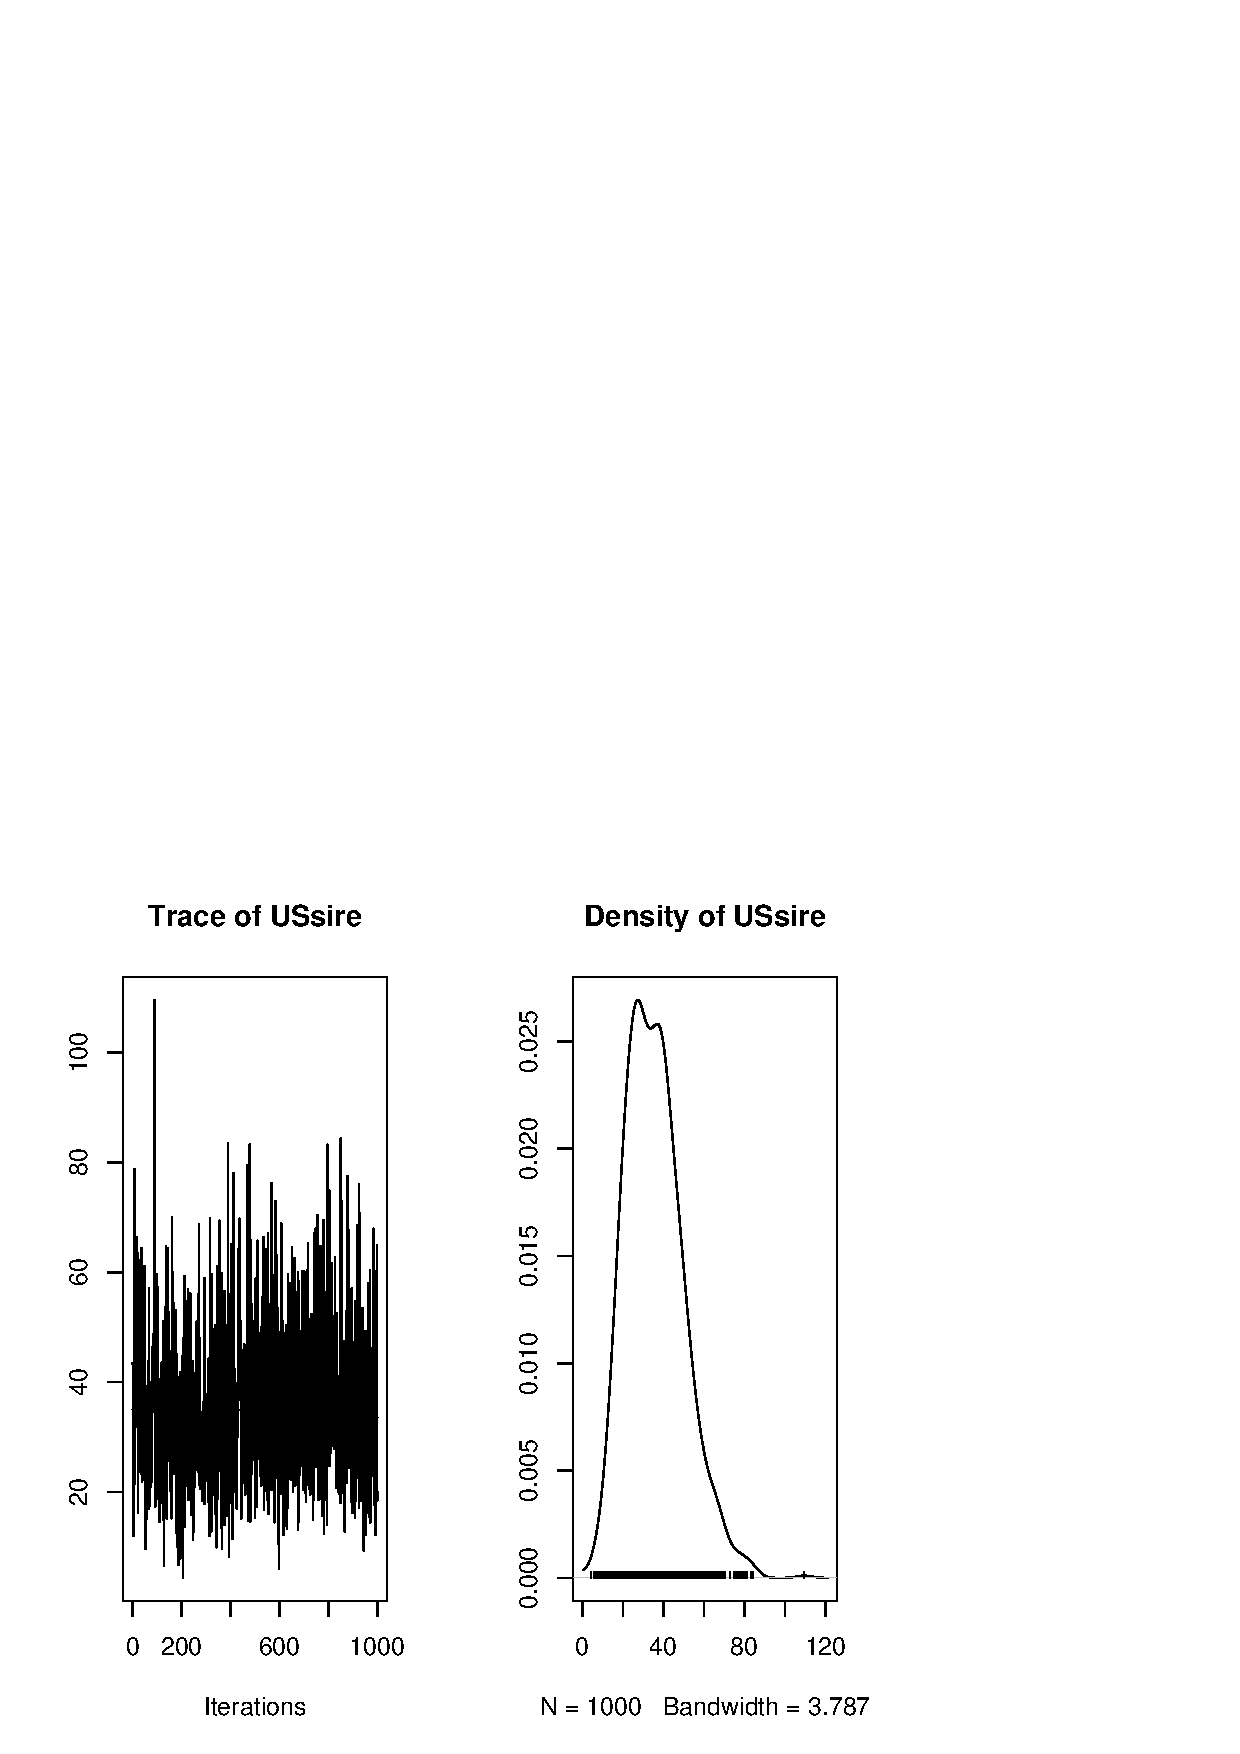
\includegraphics{Tutorial-030}
\end{center}
\caption{Posterior distribution of the number of unsampled males from \texttt{model4}. The number of unsampled males, the pedigree and $\beta$ have all been simultaneously estimated, but we have still used an approximation for genotyping error.}
\label{model4US-fig}
\end{figure}

The population of Seychelles Warbler on Cousin Island is small and essentially closed. Given that the island has been extensively sampled we have reasonable prior belief that the number of unsampled males is somewhere between 2 and 15, and an estimate of 33.79 unsampled males seems unreasonably large.  We could set up a prior specification that reflected this, but before doing this it will be usefull to discuss some possible reasons why the model has failed to estimate the number of unsampled males accurately.\\

The problem of accomodating unsampled parents is a difficult one beacuse the genotypes and phenotypes of unsampled indivduals are by definition unobserved. This does not mean that information does not exist in the observed data regarding the genotypes and phenotypes of unsampled individuals.  Imagine, that 3 offspring in the north of the island possess an allele that is not present in the sampled parental population. If genotyping error was low enough we could be reasonbaly confident in stating that an unsampled male was present in the north of the island and that his genotype contained the rare allele.  However, using this information is difficult and I use two approximations for dealing with unobserved genotypes and phenotypes that are based around the same logic.\\

\citet{Nielsen.2001} gives the likeihood of the total male population size, sampled and unsampled, given the genotype data and known mother-offspring pairs:

\begin{equation} 
Pr(\bm{G}|\bm{N}, \bm{A}) = \prod^{n_{o}}_{i}\left[\frac{N-n}{N}Pr(\bm{O}_{i}|\bm{M}_{i}, \bm{A}) + \sum_{j=1}^{n}\frac{1}{N}Pr(\bm{O}_{i}|\bm{M}_{i}, \bm{F}_{j})\right].
\label{Nielsen-eq}
\end{equation} 

$N$ and $n$ are the total and sampled male population sizes, respectively, and $n_{o}$ is the number of sampled mother-offspring pairs.  $\bm{O}$, $\bm{M}$ and $\bm{F}$ are the genotypes of offspring, mothers, and sampled father's respectively, and $\bm{A}$ are the allele frequencies in the unsampled population. The two genetic likelihoods are the Mendelian transition probability, $Pr(\bm{O}_{i}|\bm{M}_{i}, \bm{F}_{j})$, and an approximation when the genotype of a parent is unknown, $Pr(\bm{O}_{i}|\bm{M}_{i}, \bm{A})$.  This approximation makes several assumptions: a) genotype frequencies can be infered from allele frequencies under the asumption of Hardy-Weinberg equilibrium; b) the allele frequencies in the base population are known with certainty; c) genotyping error does not exist; d) the size of the unsampled population is so large that the allele frequencies in the unsampled population do not differ from $\bm{A}$; and e) $\bm{O}$ and $\bm{M}$ provide no information regarding the genotypes of unsampled males after conditioning on $\bm{A}$. Generally, $\bm{A}$ is estimated from $\bm{G}$ and an additional assumption must be made that f) unsampled males and sampled individuals come from the same statistical poulation with respect to allele frequencies.  MasterBayes makes all these assumptions except b) and c), and I return to assumption e) in Section \ref{pedigree-sec}.\\ 

We can fit Nielsen's [\citeyear{Nielsen.2001}] model using the function \texttt{MLE.popsize} by specifying the genotype error rate to be effectively zero

\begin{Schunk}
\begin{Sinput}
> MLEUSsire <- MLE.popsize(getXlist(PdP, GdP, E2 = 1e-10), USsire = TRUE, 
+     USdam = FALSE)
> MLEUSsire$nUS
\end{Sinput}
\begin{Soutput}
         [,1]
[1,] 95.24434
\end{Soutput}
\begin{Sinput}
> sqrt(MLEUSsire$C)
\end{Sinput}
\begin{Soutput}
         [,1]
[1,] 30.54465
\end{Soutput}
\end{Schunk}

Even larger! The estimates of the unsampled population size are sensitive to even low levels of genotyping error, and this is obvious when we fit the same model but with the genotyping error rate set to 0.01 per allele
  
\begin{Schunk}
\begin{Sinput}
> MLEUSsire2 <- MLE.popsize(getXlist(PdP, GdP, E2 = 0.01), USsire = TRUE, 
+     USdam = FALSE)
> MLEUSsire2$nUS
\end{Sinput}
\begin{Soutput}
         [,1]
[1,] 40.36191
\end{Soutput}
\begin{Sinput}
> sqrt(MLEUSsire2$C)
\end{Sinput}
\begin{Soutput}
         [,1]
[1,] 19.97673
\end{Soutput}
\end{Schunk}

Perhaps we had underestimated the level of genotyping error in our original models, and this possibility will be returned to in Section \ref{GE-sec}.  Another possible reason why our estimate of the unsampled population may be to high, is because Equation \ref{Nielsen-eq} makes the assumption that unsampled males and sampled males do not systematicly differ in their ability to sire the sampled offspring.\\

  When we estimate the number of unsampled males using \texttt{MCMCped} Equation \ref{Nielsen-eq} has a simpler form because the parameter space is augmented with the pedigree (See Equation \ref{pedigree-eq}):

\begin{equation}
Pr(\bm{P}|N)  = \prod^{n_{o}}_{i}\left[\frac{N-n}{N}(1-\delta^{obs}_{i})+\frac{1}{N}\delta^{obs}_{i}\right]
\label{us-eq}
\end{equation}

Here we have replaced the genetic likelihoods in Nielen's original equation with the indicator variable $\delta^{obs}_{i}$. $\delta^{obs}_{i}$ takes on the value 1 when offspring $i$'s father has been sampled, and 0 otherwise. If we knew the pedigree exactly then the Maximum Likelihood Estimate for the number of unsampled males ($N-n$) is simply the  number of offspring with unsampled fathers divided by the average number of offspring per sampled father:

\begin{equation}
\textrm{MLE}(N-n) = \frac{n_{o}^{us}n_{o}^{s}}{n}
\end{equation}

where $n_{o}^{us}$ and $n_{o}^{s}$ are the number of offspring with sampled and unsampled parents parents, respectively.\\

A more general solution than Equation \ref{us-eq} is \footnote{In earlier versions $<2.22$ this equation was wrong, as was the code. The original equation was $Pr(\bm{P}|N)  = \prod^{n_{o}}_{i}\left[\frac{N-n}{N}E\left[\frac{\hat{p}^{obs}_{i}}{\hat{p}^{miss}_{i}}\right](1-\delta^{obs}_{i})+\frac{1}{N}\delta^{obs}_{i}\right]$, and is invariant to the ratio of linear predictors. It will not have made a large difference unless unsampled parents had known phenotype.}

\begin{equation}
Pr(\bm{P}|N)  = \prod^{n_{o}}_{i}\left[\frac{N-n}{N-n+E\left[\frac{\hat{p}^{obs}_{i}}{\hat{p}^{miss}_{i}}\right]n}(1-\delta^{obs}_{i})+\frac{1}{N-n+E\left[\frac{\hat{p}^{obs}_{i}}{\hat{p}^{miss}_{i}}\right]n}\delta^{obs}_{i}\right]
\label{usgen-eq}
\end{equation}

where $\hat{p}^{obs}_{i}$ and $\hat{p}^{miss}_{i}$ are the linear predictors of paternity for sampled and unsampled males, respectively.  Nielsen's original formulation of the problem assumes that the expectaion of the ratio in Equation \ref{usgen-eq} is exactly one, and the estimate of the male population size has to be interpreted as an effective population size assuming all males to be equal.\\

The default in MasterBayes is to assume that this ratio has an expectation of 1.  However, we still need to estimate the distribution of the mean linear predictor for unsampled individuals ($\hat{p}^{miss}_{i}$) so that we can sample the pedigree correctly.\\

The parentage of each offspring is sampled from a multinomial distribution with each category representing a unique parental combination.  The probability that the offspring falls into one of these categories is based on the Mendelian transition probability and the linear predictors of potential parents.  The number of categories is equal to $(n^{o}_{d})(n^{o}_{s}+1)$ where $n^{o}_{d}$ and $n^{o}_{s}$ are the number of sampled females and males that could be the parents of offspring $o$.  An additional $n^{o}_{d}$ categories are set up in this particular example, representing the pairing of each female with an unsampled male.  The genetic likelihoods for these categories can be derived folowing Equation \ref{Nielsen-eq} and the linear predictor for this category can be derived following a similar logic.\\   

 Under the assumption that sampled and unsampled males come from the same statistical poulation,  I use an approximation based around the central limit theorem for the distribution of the linear predictor for the unsampled category.  Under the central limit theorem this distribution will be normally distributed irrespective of the underlying distribution of linear predictors when the sample size is large (equivalent to assumption a for the genetic likelihoods).  The distribution of the summed linear predictors of unsampled males can then be obtained using the following

\begin{equation}
p(\sum^{N-n}{\bm{\hat{p}}^{(miss)}} | \bm{\hat{p}}^{(obs)}) \approx N(\frac{(N-n)}{n}\sum^{n}\bm{\hat{p}}^{(obs)}, \frac{N(N-n)}{n}S_{obs}^{2})
\end{equation}

which takes into account the sampling variance in calculating the expectation from the sampled population (avoiding assumption c), and the sampling variance that arises because the size of the unsampled population is finite (assumption d). $S_{obs}^{2}$ is the sample variance of the observed linear predictors \citep[see][Chapter 7]{Gelman.2004}   I should emaphasise at this point that the approximated linear predictors for missing individuals do not enter into the likelihoood for $\beta$, they are only there to simplify the estimation of the pedigree.  However, if the phenotypes of unsampled inidviuals are known, then the linear predictors of unsampled inidviduals do not need to be estimated and can enter into the likelihood for $\beta$.  In  this insatnce the ratio in Equation \ref{usgen-eq} may not be unity and assumption f) is relaxed (See Section \ref{EPP-sec} for an example).\\

We have no information regarding the phenotypes of unsampled males in the Seychelles Warbler, and therefore the data do not allow us to distinguish between a large unsampled population and a smaller population with a reduced chance of paternity.  However, as noted earlier, the discrepancy between our estimate of 50 unsampled males and our prior belief that the number of males should be less than 15 may be a consequence of underestimating the level of genotyping error.

\subsection{Genotyping Error}
\label{GE-sec}

At this point it will be usefull to distinguish between exact and approximate methods for dealing with genotyping error.  A useful notation will be $\bm{G}$ for true but unobserved genotypes, and $\bm{G_{obs}}$ for observed but possibly erroneus genotypes.  Both methods implicitly or explicitly use this concept, and the aim is to derive the probability distribution of $\bm{G}$ from $\bm{G_{obs}}$ and what we know about error rates ($\varepsilon$) and allele frequencies ($\bm{A}$).  The approximate method defines the conditional probability of $\bm{G}$ as

\begin{equation}
Pr({\bm G} | {\bm G}_{obs}, {\varepsilon}, {\bm A})
\label{G_error_np}
\end{equation}

whereas the exact solution defines the probability as

\begin{equation}
Pr({\bm G} | {\bm G}_{obs}, {\bm P}, {\varepsilon}, {\bm A}).
\label{G_error_p}
\end{equation}

The distinction is subtle.  The approximation implicitlty assumes that the genotypes are collected from unrelated indivdiuals, whereas the exact solution acknowledges the fact that the indivdiuals are related.  By acknowledging this fact we become aware that the approximation actually throws some information away; if individuals are related then the observed genotypes of some individuals actually provide information regarding the actual genotypes of others. The exact solution comes at a computational cost.  Because the pedigree is estimated, ${\bm P}$ may change with every iteration of the Markov chain and the probability in Equation \ref{G_error_p} has to be updated each cycle.  Beacase the probability distribution of $\bm{G}$ does not depend on $\bm{P}$ in the approximation, Equation \ref{G_error_np} only needs to be evaluated once, prior to pedigree estimation.  This is only true, however, if error rates and allele frequencies (in the base population) are known with complete certainity.\\


 At this point we can drop the approximation for genotyping error and work with the exact solution, allowing us to estimate genotyping error rates and the allele frequencies in the parental generation. This becomes computationally demanding, as the probability distribution for each individual's genotype has to be calculated and sampled from each iteration of the Markov chain.  When the exact solution is used we switch from the CERVUUS model of genotyping error to one proposed by \citep{Wang.2004}.  The CERVUS model is mathematically convenient but is unlikely to be biologically realistic.  The main assumption of the CERVUS model is that an erroneous genotype is scored as another genotype (including itself) with a probability equal to that genotypes frequency in the population.  In Wang's model an allele is assumed to be misscored as any other allele with equal probability ($\varepsilon_{2}$).  In addition, the process of allelic dropout is also modelled with the probability of an allele droping out being denoted as $\varepsilon_{1}$

\begin{Schunk}
\begin{Sinput}
> model5 <- MCMCped(PdP = PdP, GdP = GdP, verbose = FALSE)
> plot(model5$E1)
> plot(model5$E2)
> plot(model5$USsire)
\end{Sinput}
\end{Schunk}


\begin{figure}[!h]
\begin{center}
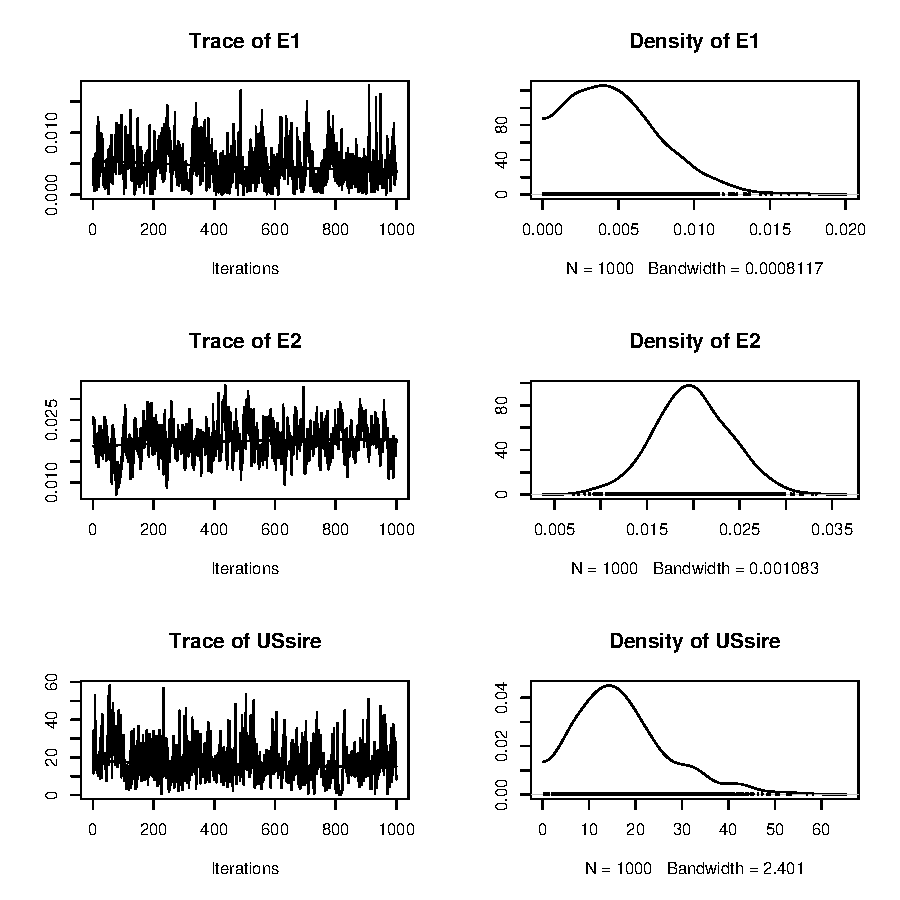
\includegraphics{Tutorial-035}
\end{center}
\caption{The marginal posterior distributions of the error rates and the number of unsampled males from \texttt{model5}. All unknowns have been simultaneously estimated.}
\label{model5-fig}
\end{figure}


The chain is slow to mix when genotypes are estimated and successive samples from the posterior show autocorrelation 

\begin{Schunk}
\begin{Sinput}
> autocorr(model5$E1)
\end{Sinput}
\begin{Soutput}
, , E1

                E1
Lag 0   1.00000000
Lag 1   0.41765511
Lag 5   0.13362918
Lag 10  0.07404815
Lag 50 -0.04446042
\end{Soutput}
\end{Schunk}

The chain needs to be run for longer to ensure that we gather independent samples from the posterior, but nethertheless it is clear that we had underestimated  the aamount of genotyping error (see Figure \ref{model5-fig}).  Allelic drop out appears to occur for about 1 in 100 genotypes, but the stochastic error rate appears higher at around 1 in 25. The posterior for the number of unsampled males now looks more reasonable but there is still alot of uncertainity and a judicious use of prior information seems reasonable.  The log normal is used as the prior specification for the number of unsampled males (see Figure \ref{model6US-fig})


\begin{Schunk}
\begin{Sinput}
> pP <- priorPed(USsire = list(mu = log(5), sigma = 0.5))
> model6 <- MCMCped(PdP = PdP, GdP = GdP, pP = pP, tP = tunePed(USsire = 0.1), 
+     verbose = FALSE)
> plot(model6$USsire)
\end{Sinput}
\end{Schunk}


\begin{figure}[!h]
\begin{center}
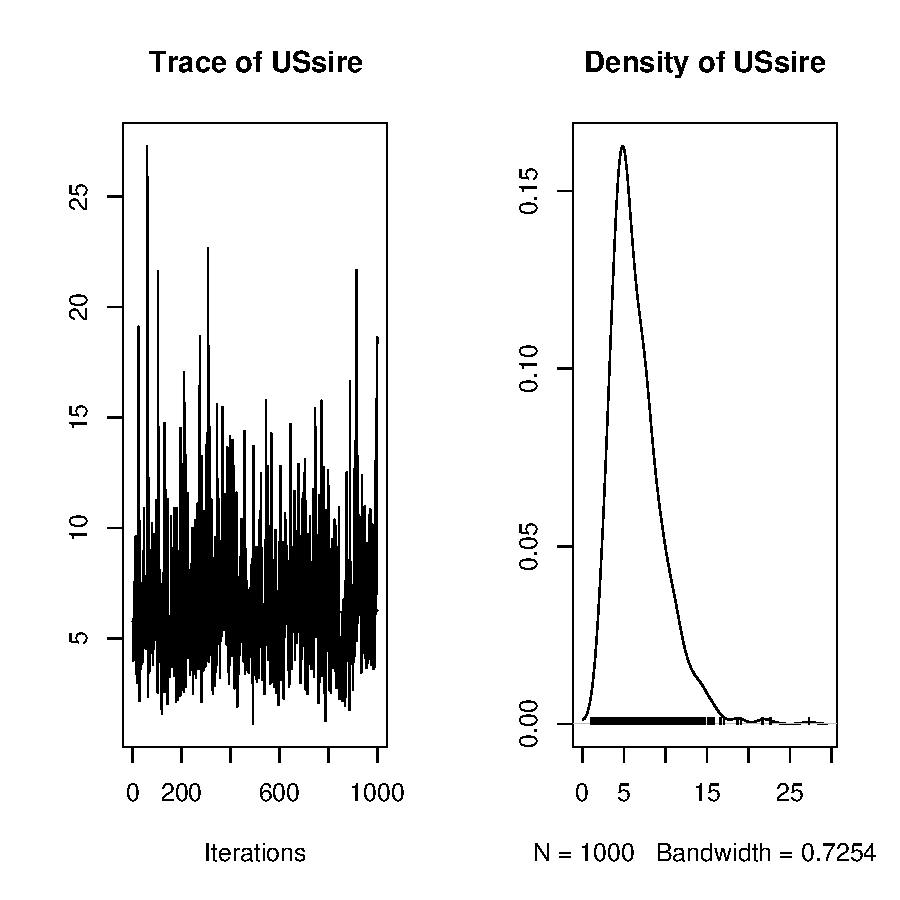
\includegraphics{Tutorial-039}
\end{center}
\caption{The marginal posterior distribution of the number of unsampled males from \texttt{model6}. In this model an informative prior was used.}
\label{model6US-fig}
\end{figure}

\section{\large{Further Examples using Simulated Data}}

To illustrate some further functionality we will use the functions \texttt{simpedigree} and \texttt{simgenotypes} to simulate pedigrees and genotypes according to certain models and then analyse them. We will use an estimate of the Seychelles Warbler allele frequencies to sample genotypes from.

\begin{Schunk}
\begin{Sinput}
> A <- extractA(WarblerG)
\end{Sinput}
\end{Schunk}

\subsection{Error Rate Estimation with and without a Pedigree}
\label{Error-sec}

 To start we will simply estimate genotyping error for two data sets, one in which the information comes from individuals being sampled multiple times and one in which the information comes from the pedigree.  We will simulate a large dropout rate (10\% of alleles in a heterozygous state) but a low level of of stochastic error  ($\approx$ 1\% of single locus genotypes).

\begin{Schunk}
\begin{Sinput}
> ped <- matrix(NA, 50, 3)
> ped[, 1] <- 1:50
> G <- simgenotypes(A = A, E1 = 0.1, E2 = 0.005, ped = ped, no_dup = 2)
> tP <- tunePed(E1 = 15)
> GdP <- GdataPed(G = G$Gobs, id = G$id)
> model.dupE <- MCMCped(GdP = GdP, tP = tP, verbose = FALSE)
> summary(model.dupE$E1)
\end{Sinput}
\begin{Soutput}
Iterations = 1:1000
Thinning interval = 1 
Number of chains = 1 
Sample size per chain = 1000 

1. Empirical mean and standard deviation for each variable,
   plus standard error of the mean:

          Mean             SD       Naive SE Time-series SE 
     0.0958506      0.0097635      0.0003087      0.0003627 

2. Quantiles for each variable:

   2.5%     25%     50%     75%   97.5% 
0.07777 0.08908 0.09567 0.10187 0.11620 
\end{Soutput}
\begin{Sinput}
> summary(model.dupE$E2)
\end{Sinput}
\begin{Soutput}
Iterations = 1:1000
Thinning interval = 1 
Number of chains = 1 
Sample size per chain = 1000 

1. Empirical mean and standard deviation for each variable,
   plus standard error of the mean:

          Mean             SD       Naive SE Time-series SE 
     4.624e-03      2.294e-03      7.254e-05      1.086e-04 

2. Quantiles for each variable:

    2.5%      25%      50%      75%    97.5% 
0.001239 0.002921 0.004238 0.005955 0.010264 
\end{Soutput}
\begin{Sinput}
> plot(model.dupE$E2)
\end{Sinput}
\end{Schunk}

The posterior summaries are consistent with the data we simulated, but notice that the mean may not be a very good summary of the central tendency of the posterior distribution for stochastic error (see Figure \ref{E2-fig})\footnote{\citet{Johnson.2007b} claim that MasterBayes overestimates error rates by 31\% when error rates are low (compared to a downward bias of 18\% for Pedant).  However, large scale simulation shows that MasterBayes is unbiased (if such a thing exists in a Bayesian analysis) if the posterior mode is used rather than the posterior mean.}. We can simulate a similar set of data but with pedigree information\\


\begin{figure}[!h]
\begin{center}
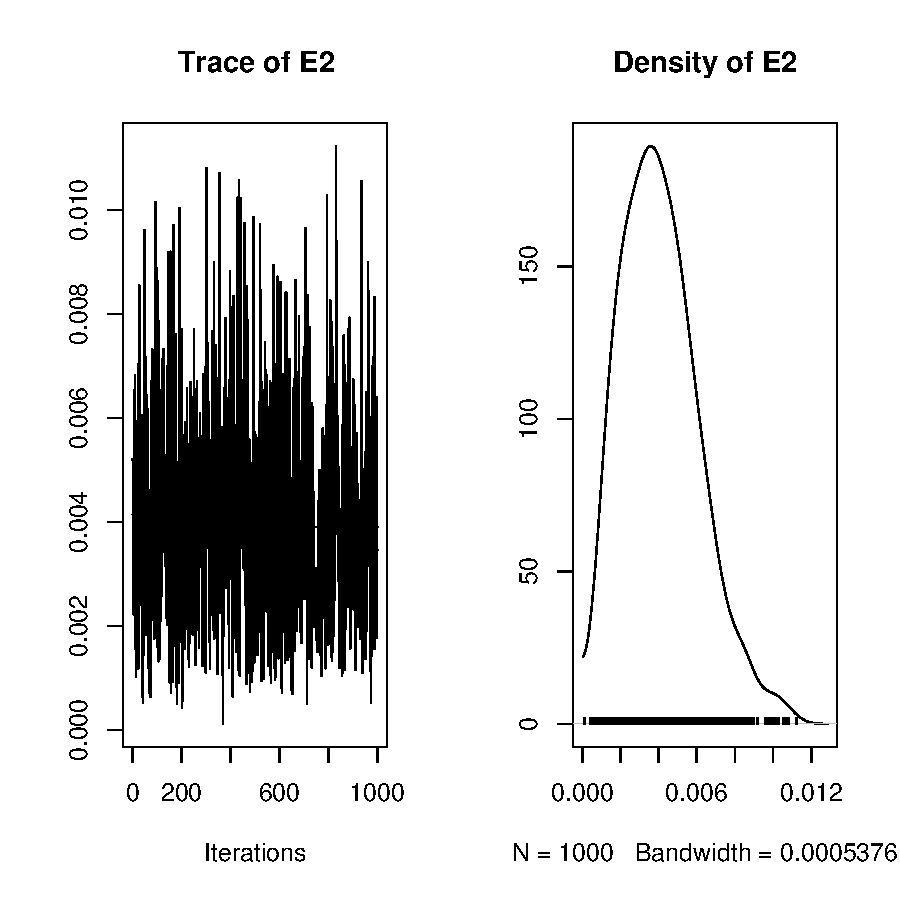
\includegraphics{Tutorial-043}
\end{center}
\caption{The marginal posterior distribution of stochastic error rate from \texttt{model.dupE}. The mode is probably a better summary of central tendency as the expectation of \texttt{E2} may not coincide with the most likely value it could take.}
\label{E2-fig}
\end{figure}

\begin{Schunk}
\begin{Sinput}
> ped <- matrix(NA, 100, 3)
> ped[, 1] <- 1:100
> ped[, 2][51:100] <- 1:50
> G <- simgenotypes(A = A, E1 = 0.1, E2 = 0.005, ped = ped, no_dup = 1)
> sP <- startPed(dam = ped[, 2])
> GdP <- GdataPed(G = G$Gobs, id = G$id)
> model.pedE <- MCMCped(GdP = GdP, sP = sP, tP = tP, verbose = FALSE)
> summary(model.pedE$E1)
\end{Sinput}
\begin{Soutput}
Iterations = 1:1000
Thinning interval = 1 
Number of chains = 1 
Sample size per chain = 1000 

1. Empirical mean and standard deviation for each variable,
   plus standard error of the mean:

          Mean             SD       Naive SE Time-series SE 
     0.0798425      0.0117579      0.0003718      0.0004700 

2. Quantiles for each variable:

   2.5%     25%     50%     75%   97.5% 
0.05774 0.07143 0.07935 0.08780 0.10261 
\end{Soutput}
\begin{Sinput}
> summary(model.pedE$E2)
\end{Sinput}
\begin{Soutput}
Iterations = 1:1000
Thinning interval = 1 
Number of chains = 1 
Sample size per chain = 1000 

1. Empirical mean and standard deviation for each variable,
   plus standard error of the mean:

          Mean             SD       Naive SE Time-series SE 
     0.0042802      0.0037796      0.0001195      0.0002858 

2. Quantiles for each variable:

     2.5%       25%       50%       75%     97.5% 
7.568e-05 1.428e-03 3.223e-03 6.312e-03 1.342e-02 
\end{Soutput}
\end{Schunk}

The posterior from the second data set has greater variance.  With respect to genotyping error, multiple samples from the same individual are more informative than genotypes typed once in mother-offspring pairs.  If individuals have been typed more than once then this information should be included in pedigree reconstruction as it improves error rate estimation and increases the precision with which an indivdiual's genotype is estimated.\\

In Section \ref{MCMC.D-sec} I mentioned the fact that MCMC may be sensitive to the starting parameterisation, and that this is particularly so when the posterior distribution is high-dimensional and multimodal.  The posterior distribution of genotypes has these properties, and high probability genotype configurations may seperated by regions of zero probability when pedigree data exist.  As an example we will specify a random (but legal) starting configuration for the previous model:

\begin{Schunk}
\begin{Sinput}
> stG <- simgenotypes(A = A, E1 = 0, E2 = 0, ped = ped, no_dup = 1)
> sP <- startPed(dam = ped[, 2], G = stG$Gobs)
> model.config <- MCMCped(GdP = GdP, sP = sP, tP = tP, verbose = FALSE)
> plot(model.config$E2)
\end{Sinput}
\end{Schunk}



\begin{figure}[!h]
\begin{center}
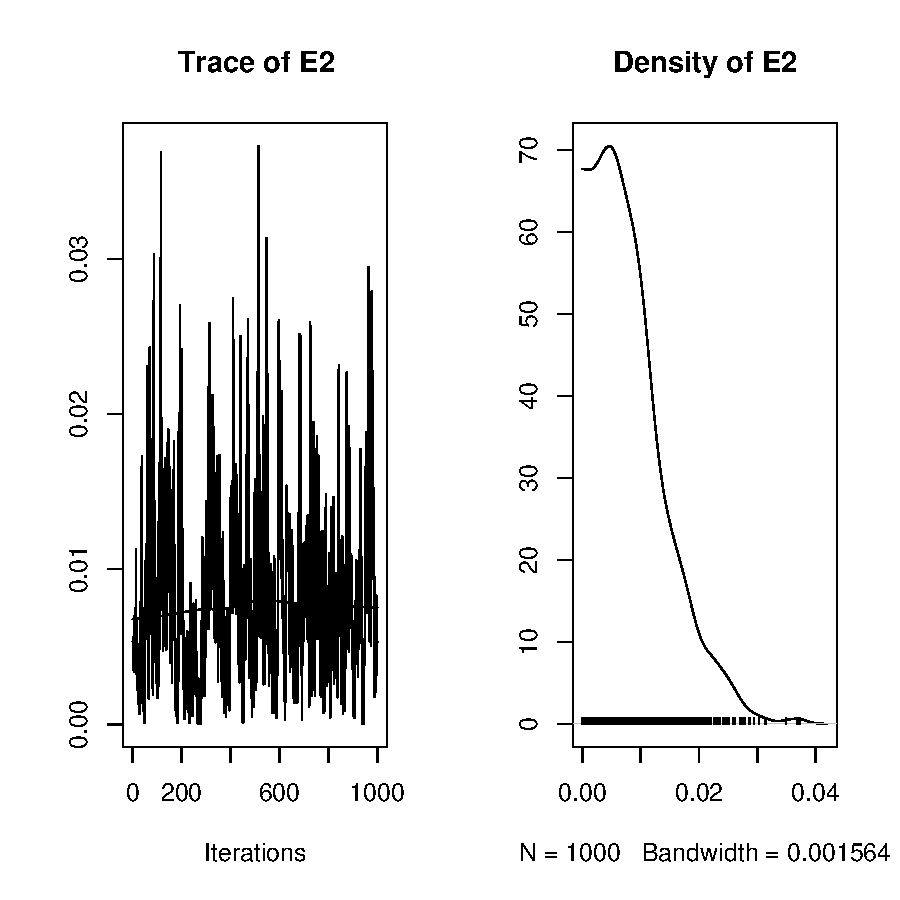
\includegraphics{Tutorial-047}
\end{center}
\caption{The marginal posterior distribution of stochastic error rate from \texttt{model.config}. This posterior should be identical to the posterior in Figure \ref{E2-fig}, although the chain was initilised in a very low probability region of genotype parameter space.}
\label{E2con-fig}
\end{figure}

When only dams are known the chain still mixes well and the chain converges very rapidly despite the absurd starting configuration (see Figure \ref{E2con-fig}).  However, we can simulate genotypes down a pedigree when both dams and sire are known.  We will analyse the data using two chains, one initialised at the true genotype configuration, and one initialised at a random but legal configuration.

\begin{Schunk}
\begin{Sinput}
> ped <- matrix(NA, 150, 3)
> ped[, 1] <- 1:150
> ped[, 2][101:150] <- 1:50
> ped[, 3][101:150] <- 51:100
> G <- simgenotypes(A = A, E1 = 0.1, E2 = 0.005, ped = ped, no_dup = 1)
> sP <- startPed(dam = ped[, 2], sire = ped[, 3], G = G$G)
> GdP <- GdataPed(G = G$Gobs, id = G$id)
> model.DS1 <- MCMCped(GdP = GdP, sP = sP, tP = tP, verbose = FALSE)
> stG <- simgenotypes(A = A, E1 = 0.1, E2 = 0.005, ped = ped, no_dup = 1)
> sP <- startPed(dam = ped[, 2], sire = ped[, 3], G = stG$G)
> model.DS2 <- MCMCped(GdP = GdP, sP = sP, tP = tP, verbose = FALSE)
> post.max <- max(c(model.DS1$E2, model.DS2$E2))
> plot(c(model.DS1$E2), type = "l", col = "blue", ylim = c(0, post.max))
> lines(c(model.DS2$E2), type = "l", col = "red")
\end{Sinput}
\end{Schunk}



\begin{figure}[!h]
\begin{center}
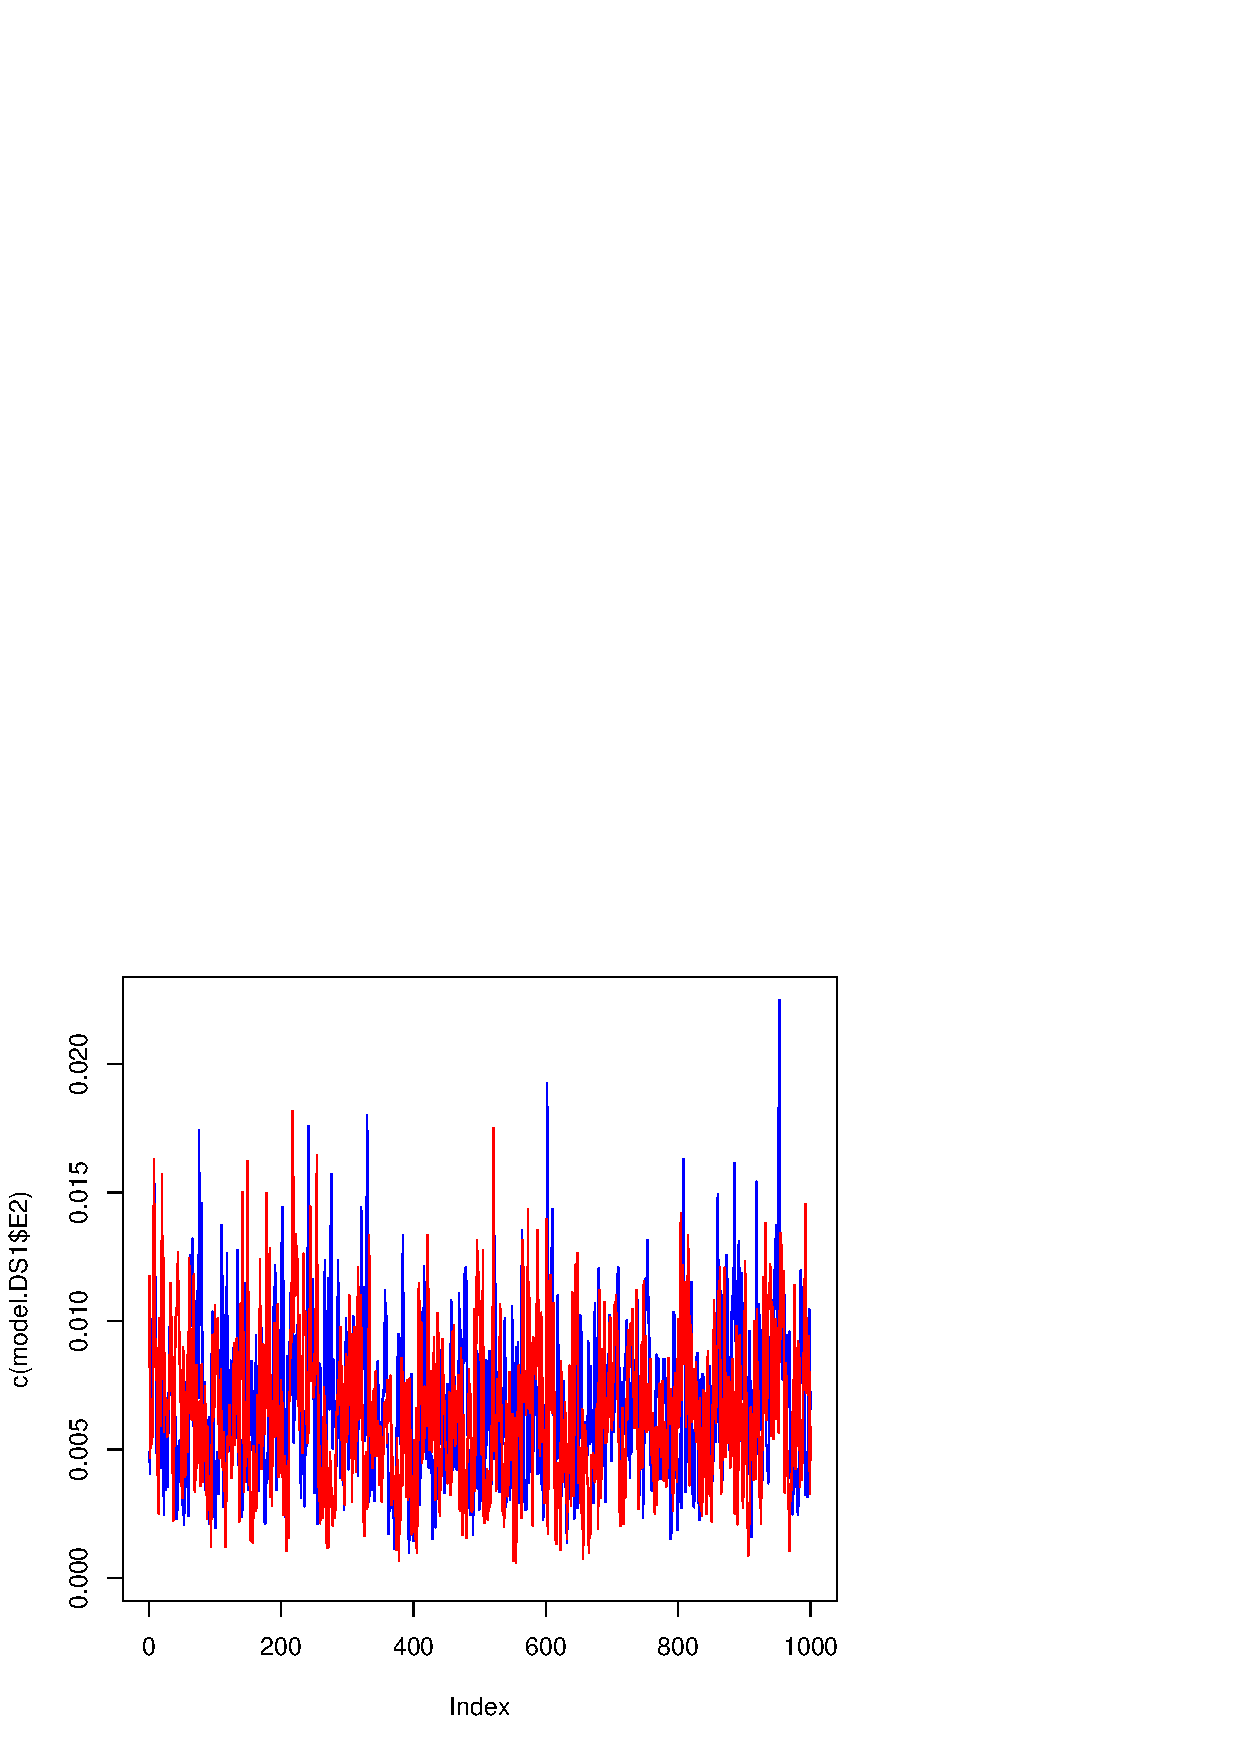
\includegraphics{Tutorial-050}
\end{center}
\caption{Samples from the posterior distribution of stochastic error rate estimated from the data set \texttt{Gobs}. The two chains were initialised at the true genotype configuration (blue), and a random congiguartion (red).} 
\label{E2DS-fig}
\end{figure}

Clearly, the chains are sampling from different regions of the posterior (Figure \ref{E2DS-fig}).  Methods exist for traversing these regions \citep{Sheehan.2000, Lange.2002} but these are hard to implement on fixed pedigrees, let alone pedigrees that are being constantly updated.  However, when the pedigree is not fixed, zero probability regions do not exist because all genotype congigurations have a positive probability under some pedigree configuration.  Nethertheless, there may be regions of very low probability connecting high probability regions, and the chain may not mix well.  

\subsection{Mismatch Tolerence and Computational Efficency}

The number of potential parental combinations is not linear in the number of potential mothers and fathers.  With 50 candidate mothers and 50 candidate fathers the number of parental combinations is 2500.  This can slow the chain down because each iteration, and for each offspring 2500 Mendelian likelihoods have to be recalculated.  Also, we have to sample parents from a multinomial distribution with as many categories.  When genotyping error is low, we can safely assume that potential parents that have many mismatches with an offspring have a probability close to zero of being the true parents.  The argument \texttt{mm.tol} can be passed to \texttt{MCMCped} specifying the number of mismatches that will be tolerated for a potential parent\footnote{Later versions of MasterBayes ($>2.1$) also include the argument \texttt{jointP}. When \texttt{jointP=FALSE} then an alternative Gibbs sampler is used which samples dams conditional on sires, followed by sires conditional on dams.  The chain may mix slower (per number of iterations) than the default \texttt{jointP=TRUE}, but the chain may iterate much faster if $n_{i}n_{j}>>n_{i}+n_{j}$, where $n_{i}$ and $n_{j}$ are the number of potential dams and sires.}.\\

To illustrate I have simulated a pedigree where body size has a strong effect on both paternity and maternity.  However, the effect of body size is not the same for the sexes: large males have an increased chance of gaining paternity, but small females are more fecund. Following the notation of Equation \ref{dist-eq}:

\begin{equation}
p^{(o)}_{i,j} \propto \textrm{exp}(\beta_{1}\textrm{\texttt{size}}_{i} + \beta_{2}\textrm{\texttt{size}}_{j})
\end{equation}

A pedigree is simulated with $\beta_{1}$ and $\beta_{2}$ set to -1 and 1, respectively.

\begin{Schunk}
\begin{Sinput}
> sex <- c(rep("Female", 50), rep("Male", 100))
> offspring <- c(rep(0, 100), rep(1, 50))
> size <- rnorm(150, 10)
> data.MM <- as.data.frame(list(id = 1:150, sex = sex, offspring = offspring, 
+     size = size))
> res1 <- expression(varPed(x = "offspring", restrict = 0))
> var1 <- expression(varPed(x = "size", gender = "Male"))
> var2 <- expression(varPed(x = "size", gender = "Female"))
> PdP <- PdataPed(formula = list(res1, var1, var2), data = data.MM)
> simped <- simpedigree(PdP, beta = c(1, -1))
> G <- simgenotypes(A = A, E1 = 0.005, E2 = 0.005, ped = simped$ped, 
+     no_dup = 1)
> GdP <- GdataPed(G = G$Gobs, id = G$id)
> model_pedMM999 <- MCMCped(PdP = PdP, GdP = GdP, verbose = FALSE)
> model_pedMM2 <- MCMCped(PdP = PdP, GdP = GdP, mm.tol = 2, verbose = FALSE)
> model_pedMM1 <- MCMCped(PdP = PdP, GdP = GdP, mm.tol = 1, verbose = FALSE)
> summary(model_pedMM999$beta)[[1]][, 1:2][1:2, ]
\end{Sinput}
\begin{Soutput}
             Mean        SD
size.D  0.9487343 0.1564830
size.S -0.8567577 0.1290054
\end{Soutput}
\begin{Sinput}
> summary(model_pedMM2$beta)[[1]][, 1:2][1:2, ]
\end{Sinput}
\begin{Soutput}
             Mean        SD
size.D  0.9666110 0.1616535
size.S -0.8644591 0.1225466
\end{Soutput}
\begin{Sinput}
> summary(model_pedMM1$beta)[[1]][, 1:2][1:2, ]
\end{Sinput}
\begin{Soutput}
             Mean        SD
size.D  0.9585069 0.1660709
size.S -0.8569236 0.1225317
\end{Soutput}
\end{Schunk}

The posterior distributions of $\beta$ are almost identical, despite excluding parents with several mismatches. However, the saving in computer time was large: the first model took almost 15 minutes to fit where the last model took under 3. 

\subsection{Equivalence with Poisson Models}

 If we knew the pedigree we may be inclined to fit a generalised linear model with a Possion error distribution and log link to the data set \texttt{data.MM}.  We can analyse the relationship between female body size and fecundity by counting the number of offspring per female, and using the standard \texttt{glm} function in R 

\begin{Schunk}
\begin{Sinput}
> counts <- rep(0, 50)
> noff <- table(simped$ped[, 2])
> counts[as.numeric(names(noff))] <- counts[as.numeric(names(noff))] + 
+     noff
> model.Pd <- glm(counts ~ size[1:50], family = "poisson")
> summary(model.Pd)
\end{Sinput}
\begin{Soutput}
Call:
glm(formula = counts ~ size[1:50], family = "poisson")

Deviance Residuals: 
    Min       1Q   Median       3Q      Max  
-1.7051  -0.8373  -0.6440   0.4065   1.9651  

Coefficients:
            Estimate Std. Error z value Pr(>|z|)    
(Intercept)  -9.7396     1.6199  -6.012 1.83e-09 ***
size[1:50]    0.9308     0.1477   6.304 2.91e-10 ***
---
Signif. codes:  0 '***' 0.001 '**' 0.01 '*' 0.05 '.' 0.1 ' ' 1 

(Dispersion parameter for poisson family taken to be 1)

    Null deviance: 86.281  on 49  degrees of freedom
Residual deviance: 42.987  on 48  degrees of freedom
AIC: 108.86

Number of Fisher Scoring iterations: 5
\end{Soutput}
\end{Schunk}

The slopes are virtually the same,  but the standard errors are a little larger for the \texttt{MCMCped} model, reflecting uncertainity in the pedigree.  However, because size is such a good predictor of parentage, and the genotype data are relatively informative, the pedigree is resolved quite well.

\begin{Schunk}
\begin{Sinput}
> table(simped$ped[, 2:3][101:150, ] == modeP(model_pedMM999$P)[, 
+     2:3])
\end{Sinput}
\begin{Soutput}
FALSE  TRUE 
   12    88 
\end{Soutput}
\end{Schunk}

The modal parenatge assignments are close to the true pedigree, with 88\% of assignments correct. One important difference arises because \texttt{MCMCped} uses a mutinomial log-linear model rather than the Poisson log-linear model used above.  The models are very similar except the multinomial model conditions on the number of counts (offspring) whereas the Possion model does not. Consequently the number of parameters in a multinomial model (excluding the count total) is one less than the equivalent Poisson model. In the above example an intercept term is not calculated becuase it can be derived directly from the number of parental combinations and the number of offspring which we have conditioned on \citep{McCullagh.1989}.  

\subsection{Interactions and Reparameterisation}

Next we will consider a model similar to that above, but we will have a constant effect of size for both sexes.  However, we will incude a second variable \texttt{age} which has two levels: \texttt{old} and \texttt{young}. We will fit both main effects together with an interaction.  Interactions can fitted by adding an extra element to the \texttt{formula} argument that is list containing the two \texttt{varPed} expressions to be combined \footnote{In earlier versions of MasterBayes ($<2.2$) interactions could only be fitted when both terms were included as main effects.  In later versions interactions can be fitted without main effects. This type of model is more appropriate if for example, you want to test whether pollen dispersal differs between years. In this model you would be interested in fitting a year by distance interaction and the main effect of distance, but generally fitting a main effect of year is not appropriate.}.\\

\begin{equation}
p^{(o)}_{i,j} \propto \textrm{exp}(\beta_{1}\delta_{i}+\beta_{1}\delta_{j}+\beta_{2}\textrm{\texttt{size}}_{i}\delta_{i}+\beta_{2}\textrm{\texttt{size}}_{j}\delta_{j}+\beta_{3}\textrm{\texttt{size}}_{i}(1-\delta_{i})+\beta_{3}\textrm{\texttt{size}}_{j}(1-\delta_{j}))
\label{int-eq}
\end{equation}

The $\delta$ variables take on the values 1 if the individual is young, and zero if not.  Notice that although there are six terms in Equation \ref{int-eq} there only 3 parameters to be estimated because the variables are assumed to have consistent effects on both maternity and paternity.   


\begin{Schunk}
\begin{Sinput}
> age <- gl(2, 1, 150, label = c("old", "young"))
> data_INT <- cbind(data.MM, age)
> res1 <- expression(varPed(x = "offspring", restrict = 0))
> var1 <- expression(varPed(x = "size"))
> var2 <- expression(varPed(x = "age"))
> PdP <- PdataPed(formula = list(res1, var1, var2, list(var1, var2)), 
+     data = data_INT)
> simped <- simpedigree(PdP, beta = c(0.5, 10, -1))
> G <- simgenotypes(A = A, E1 = 0.005, E2 = 0.005, ped = simped$ped, 
+     no_dup = 1)
> GdP <- GdataPed(G = G$Gobs, id = G$id)
> model.INT <- MCMCped(PdP = PdP, GdP = GdP, mm.tol = 1, verbose = FALSE)
\end{Sinput}
\end{Schunk}

Markov chains do not mix well when the posterior distribution of the parameters are not independent. Indeed, the autocorrelation approaches 1 despite a thinning interval of 10 (See Figure \ref{INT-fig}).

\begin{Schunk}
\begin{Sinput}
> plot(model.INT$beta)
> autocorr(model.INT$beta)[, , 3]
\end{Sinput}
\begin{Soutput}
               size   age.young size.age.young
Lag 0  -0.679447739 -0.99182549    1.000000000
Lag 1  -0.168695476 -0.27650174    0.276980894
Lag 5  -0.008297778 -0.04498004    0.049770485
Lag 10  0.045420532  0.01070933   -0.005485801
Lag 50 -0.008027279 -0.02455821    0.022886000
\end{Soutput}
\end{Schunk}



\begin{figure}[!h]
\begin{center}
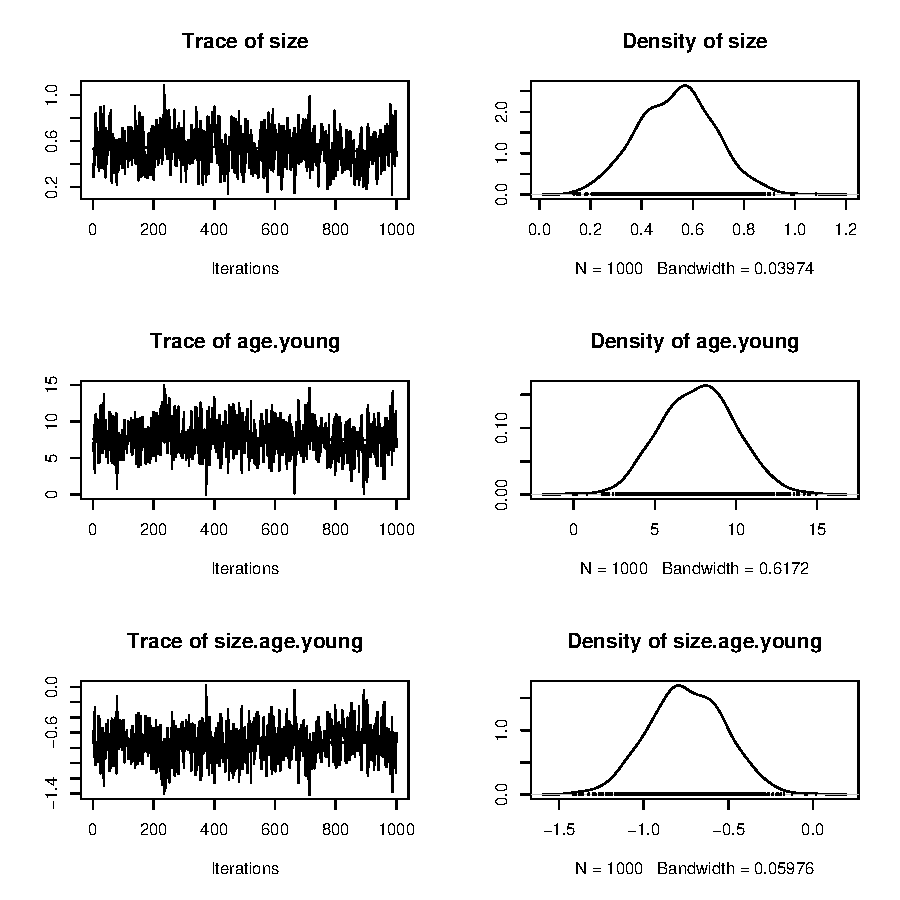
\includegraphics{Tutorial-057}
\end{center}
\caption{The marginal posterior distributions for the three elements of \texttt{beta} from \texttt{model.INT}.  The intercpet for young individuals \texttt{age.young} is evaluated at a \texttt{size} of 0, which lies well outside the distribution of \texttt{size} observed in the population.}
\label{INT-fig}
\end{figure}

The dependency between slopes and intercpets in regression models is well know and we can alleviate the problem by simply centering the covariate, \texttt{size}.  The intercept is now evaluated at the population mean for size (10) rather than at a size of zero

\begin{Schunk}
\begin{Sinput}
> data_INT[, "size"] <- size - 10
> PdP <- PdataPed(formula = list(res1, var1, var2, list(var1, var2)), 
+     data = data_INT)
> model.INT.cntr <- MCMCped(PdP = PdP, GdP = GdP, mm.tol = 1, verbose = FALSE)
> plot(model.INT.cntr$beta)
> autocorr(model.INT.cntr$beta)[, , 3]
\end{Sinput}
\begin{Soutput}
                size    age.young size.age.young
Lag 0  -0.6833482238 -0.034066030     1.00000000
Lag 1  -0.1562431963 -0.009102893     0.28964502
Lag 5   0.0003164919 -0.005746424    -0.03614487
Lag 10  0.0372870968  0.021355725    -0.05675842
Lag 50 -0.0512534320 -0.053455951     0.02039196
\end{Soutput}
\end{Schunk}


\begin{figure}[!h]
\begin{center}
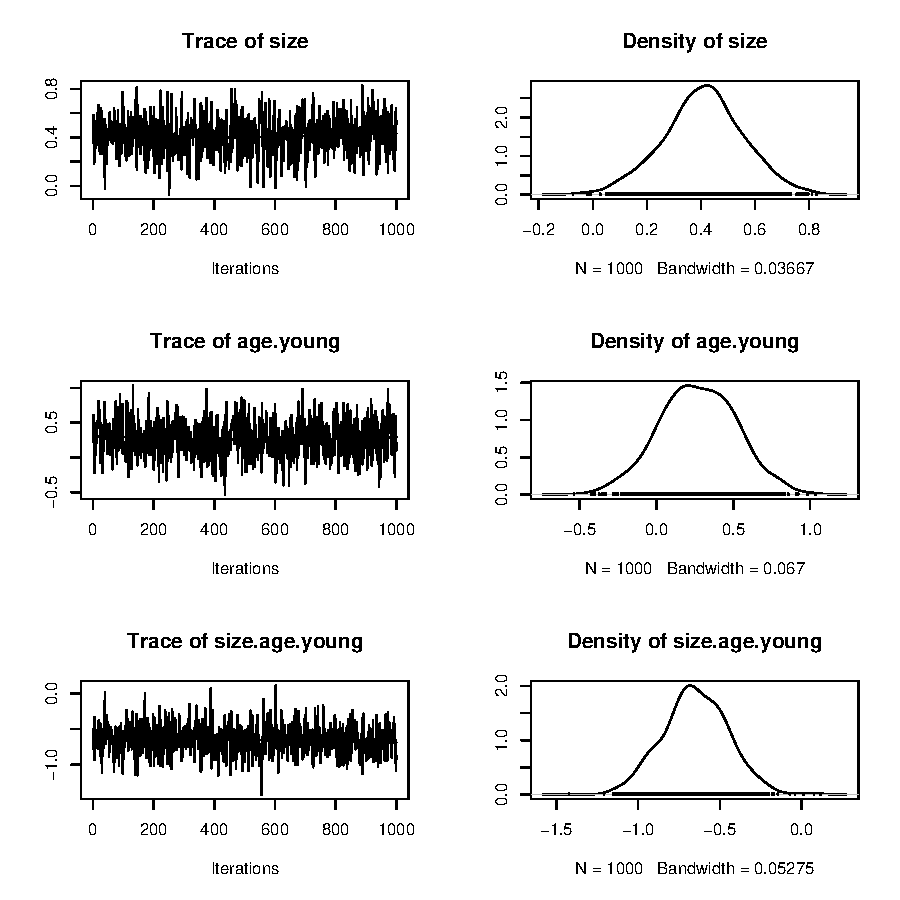
\includegraphics{Tutorial-060}
\end{center}
\caption{The marginal posterior distributions for the three elements of \texttt{beta} from \texttt{model.INT}, but with the intercpet for young individuals \texttt{age.young} evaluated at the average \texttt{size} of 10.  }
\label{INT.cntr-fig}
\end{figure}

Despite having similiar Metropolis-Hastings acceptance rates the second chain mixes much better, and the parameters have a better biological interpretation: at the average size no differences in the ability to reproduce exists between young and old individuals;  the posterior distribution of \texttt{age.young} is centered around zero (Figure \ref{INT.cntr-fig}).  However, as old individuals get larger their ability to reproduce increases (\texttt{size} is positive - the true underlying slope is 0.5), but young indivdiuals have a significantly shallower slope (\texttt{size.age.young} is less than zero).  The contrasts are set up so that \texttt{size.age.young} is is the differnce between the slopes of young and old inidviduals.  Inference from posterior samples is very flexible.  If we wish to see whether the slope is so shallow it is in fact likely to be negative we can create the posterior distribution for the young slope

\begin{Schunk}
\begin{Sinput}
> young.slope <- mcmc(model.INT.cntr$beta[, 1] + model.INT.cntr$beta[, 
+     3])
> plot(young.slope)
\end{Sinput}
\end{Schunk}


\begin{figure}[!h]
\begin{center}
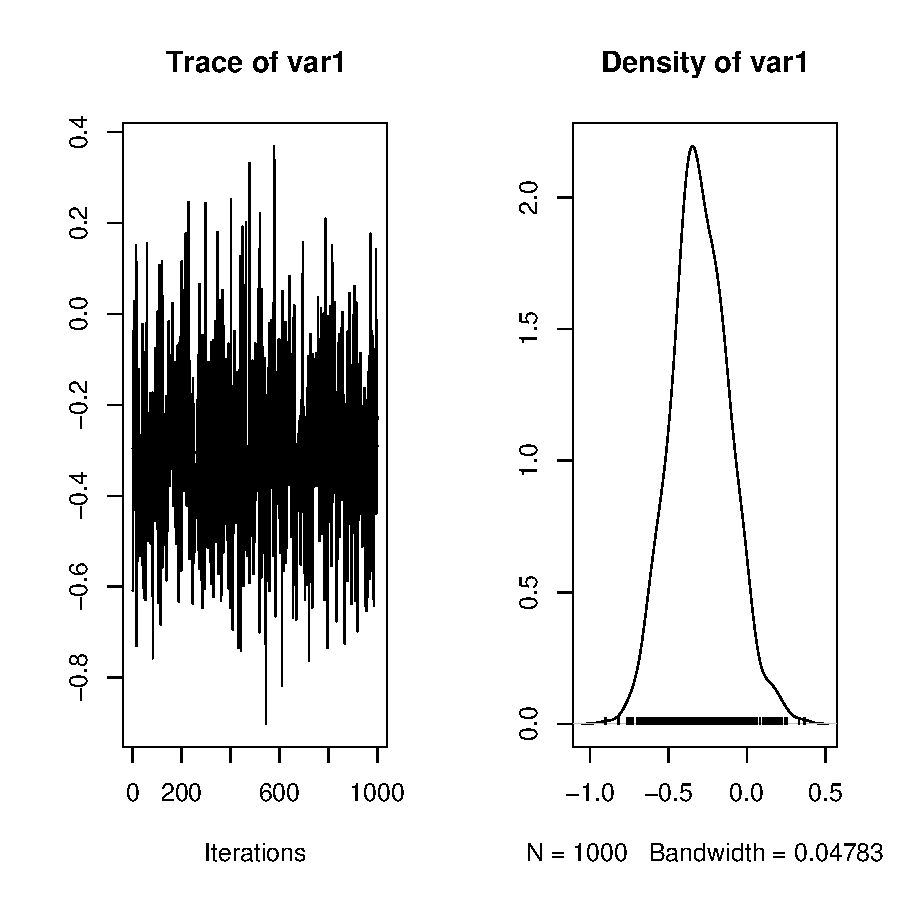
\includegraphics{Tutorial-063}
\end{center}
\caption{The marginal posterior distribution for the slope of young individuals from model \texttt{model.INT.cntr}.}
\label{ys-fig}
\end{figure}

There is good evidence that the slope for young individuals is negative (Figure \ref{ys-fig}).  In fact the pedigree was simulated so that the slopes would be of the same magnitude (0.5), but with different signs. In this instance the sexes followed the same rules with regard to reproduction, and we can fit a single GLM across the sexes

\begin{Schunk}
\begin{Sinput}
> counts <- rep(0, 100)
> noff <- table(c(simped$ped[, 2], simped$ped[, 3]))
> counts[as.numeric(names(noff))] <- counts[as.numeric(names(noff))] + 
+     noff
> par_age <- age[1:100]
> par_size <- size[1:100] - 10
> model.Pint <- glm(counts ~ par_age * par_size, family = "poisson")
> summary(model.Pint)
\end{Sinput}
\begin{Soutput}
Call:
glm(formula = counts ~ par_age * par_size, family = "poisson")

Deviance Residuals: 
     Min        1Q    Median        3Q       Max  
-1.85658  -1.16297  -0.07152   0.61389   2.45469  

Coefficients:
                      Estimate Std. Error z value Pr(>|z|)    
(Intercept)            -0.1857     0.1636  -1.136 0.256104    
par_ageyoung            0.1478     0.2223   0.665 0.506146    
par_size                0.3676     0.1359   2.705 0.006838 ** 
par_ageyoung:par_size  -0.6878     0.1856  -3.705 0.000211 ***
---
Signif. codes:  0 '***' 0.001 '**' 0.01 '*' 0.05 '.' 0.1 ' ' 1 

(Dispersion parameter for poisson family taken to be 1)

    Null deviance: 112.684  on 99  degrees of freedom
Residual deviance:  98.845  on 96  degrees of freedom
AIC: 254.14

Number of Fisher Scoring iterations: 5
\end{Soutput}
\end{Schunk}

A Poisson GLM indicates the same thing: young and old indivdiuals do not appear to behave differently at the average body size.  However, the slope for old individuals is significantly positive, and the slope for young individuals differs significantly from the slope of old indivdiuals. Testing whether young individuals have a negative slope would involve setting different contrasts. 

\subsection{Interpreting Parameters Associated with Categorical Variables}

Imagine an experiment in which 30 males are randomly selected from a large population and treated, and we are interested in whether the treatment affects fecundity.  We would like a statistic that does not depend on the number of treated and control males in the population.  We are not interested in the probability that an offspring has a treated father compared to a control father, because this probability could be increased by simply treating a greater proportion of males.  The default in MasterBayes is to estimate the logs odd ratio ($\beta$) of a male siring an offspring if that male had been treated compared to if it had been left untreated, where

\begin{equation}
\beta  = log\left[\frac{\theta}{1-\theta}\right] = logit(\theta)
\end{equation}

and $\theta$ is the probability if that male had been treated. A nice property of posterior distributions is that we can take the inverse logit transformation of the samples gathered for the posterior distribution of $\beta$ to make valid inferences about the posterior of $\theta$.\\

When the number of treated ($N_{E}$) and untreated ($N_{C}$) potential fathers is known, and does not vary between offspring we can derive the probability that an offspring will be sired by a treated male ($\theta_{o}$):

\begin{equation}
\theta_{o}  = \frac{\theta N_{E}}{\theta N_{E} + (1-\theta)N_{C}},  
\label{eq_thetao}
\end{equation}

and also the logs odd ratio

\begin{equation}
\beta_{o}  = logit(\theta_{o})
\end{equation}

By default MasterBayes estimates $\beta$, although $\beta_{o}$ can be estimated using the argument \texttt{merge=TRUE} in \texttt{varPed}.  When the number of experimental and non-experimental males are known, and the sets of potential fathers for all offspring are equal, there is no statistical reason for choosing $\beta$ over $\beta_{o}$ since they are functionally equivalent.  However, there are cases when $\beta$ and $\beta_{o}$ are not equivalent and care needs to be taken when choosing between the two models.  A classic example of when  $\beta_{o}$ would be favoured over $\beta$ is when estimating the level of extra-pair paternity.
 


\subsection{Unsampled Parents with Known Phenotypes: Estimating Extra-pair Paternity}
\label{EPP-sec}

Consider a study site with 50 territories, each of which contains a pair of adults.  We will assume that the mother of all offspring on a given territory is the territorial female, but some offspring may be sired by males from another territory.  Let's imagine that we have sampled all the individuals on half the territories, and would like to know a) the extra-pair paternity rate, and b) the number of unsampled territories, which in this case is 25. We will start by simulating a pedigree with an extra-pair paternity rate of 20\%.

\begin{Schunk}
\begin{Sinput}
> sex <- c(rep("Male", 50), rep("Female", 125))
> terr <- as.factor(c(1:50, 26:50, rep(26:50, each = 4)))
> offspring <- c(rep(0, 75), rep(1, 100))
> data_EPP <- as.data.frame(list(id = 1:175, sex = sex, offspring = offspring, 
+     terr = terr))
> res1 <- expression(varPed(x = "terr", gender = "Female", relational = "OFFSPRING", 
+     restrict = "=="))
> var1 <- expression(varPed(x = "terr", gender = "Male", relational = "OFFSPRING"))
> res2 <- expression(varPed(x = "offspring", restrict = 0))
> PdP <- PdataPed(formula = list(res1, var1, res2), data = data_EPP)
> EPP <- 0.8/(0.8 + (0.2/49))
> simped <- simpedigree(PdP, beta = logit(EPP))
> G <- simgenotypes(A = A, E1 = 0.01, E2 = 0.01, ped = simped$ped, 
+     no_dup = 1)
> GdP <- GdataPed(G = G$Gobs, id = G$id)
> rm_males <- 1:25
> data_EPP_miss <- data_EPP[-rm_males, ]
> GdP_miss <- GdataPed(G = lapply(G$Gobs, function(x) {
+     x[-rm_males]
+ }), id = G$id[-rm_males])
\end{Sinput}
\end{Schunk}

Notice the argument \texttt{merge=FALSE} is passed to \texttt{varPed} for \texttt{var1} indicating that we are estimating $\beta$,  not the within-pair paternity rate which in this case is $\beta_{o}=0.8$. Also, we are treating the unsampled males as if they came from the same statistical population as the sampled males (\texttt{USvar=NULL}), although we know that the logical variable indicating whether offspring and males are on the same territory should be \texttt{FALSE} for unsampled males.
  
\begin{Schunk}
\begin{Sinput}
> PdP_miss <- PdataPed(formula = list(res1, var1, res2), data = data_EPP_miss, 
+     USsire = TRUE)
> model.miss <- MCMCped(PdP = PdP_miss, GdP = GdP_miss, verbose = FALSE)
> plot(model.miss$beta)
> plot(model.miss$USsire)
\end{Sinput}
\end{Schunk}


\begin{figure}[!h]
\begin{center}
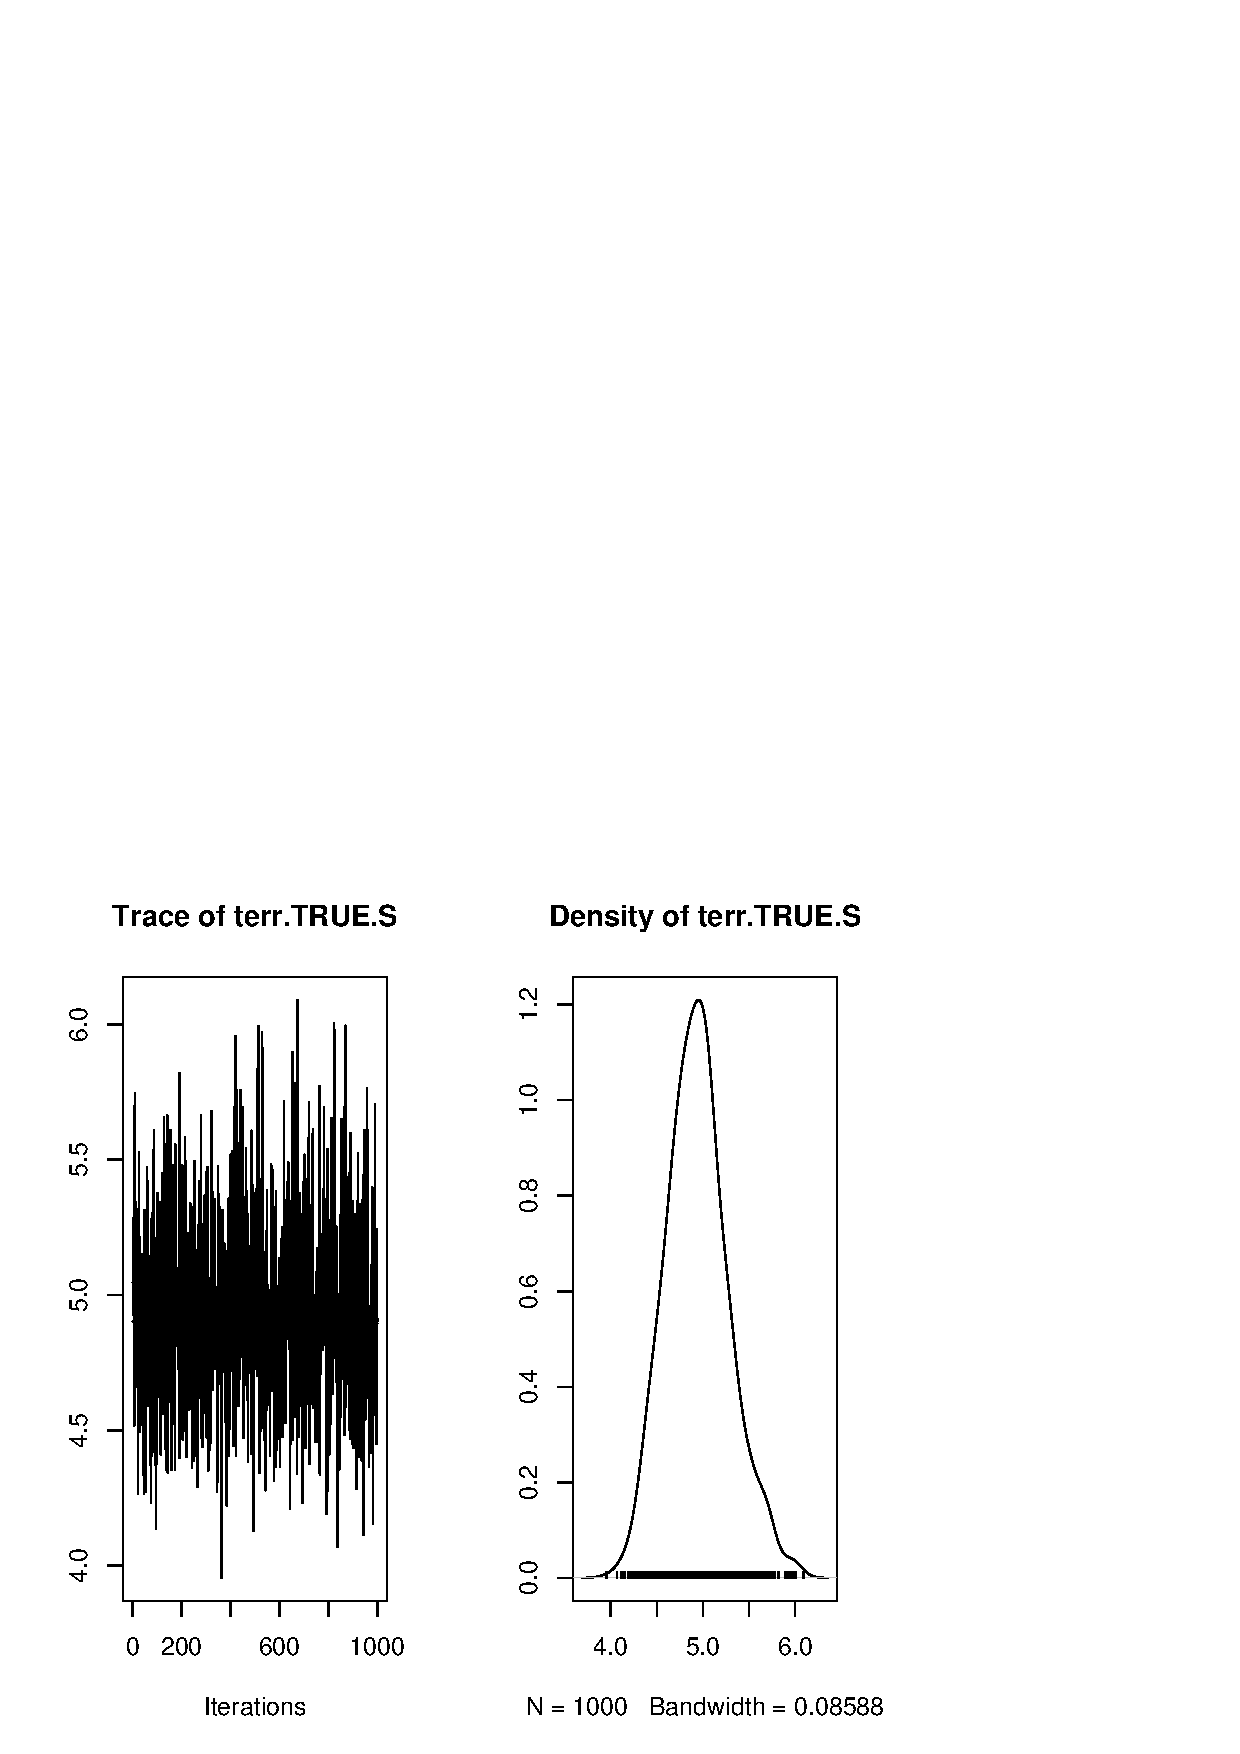
\includegraphics{Tutorial-068}
\end{center}
\caption{The marginal posterior distribution of $\beta$ from \texttt{model.miss}.  This is the log odds ratio of a male scoring paternity if it had been on the offspring's territory compared to if it had been on a different territory. The pedigree is sampled assuming that the phenotypes of unsampled males are unknown.}
\label{EPP1-fig}
\end{figure}


The estimate of $\beta$ seems reasonable given that \texttt{logit(EPP)=5.28} (Figure \ref{EPP1-fig}), but the number of unsampled males is much smaller than we anticipated (Figure \ref{EPP1US-fig}).  This is beacuse we left \texttt{USvar=NULL}, and approximated the summed linear predictors of unsampled males from the linear predictors of sampled males (see Section \ref{us-sec}).  In fact the probability that an unsampled male gains paternity over a sampled male are not equal, since unsampled males are always extra-pair fathers but sampled males may be within-pair fathers.\\  


\begin{figure}[!h]
\begin{center}
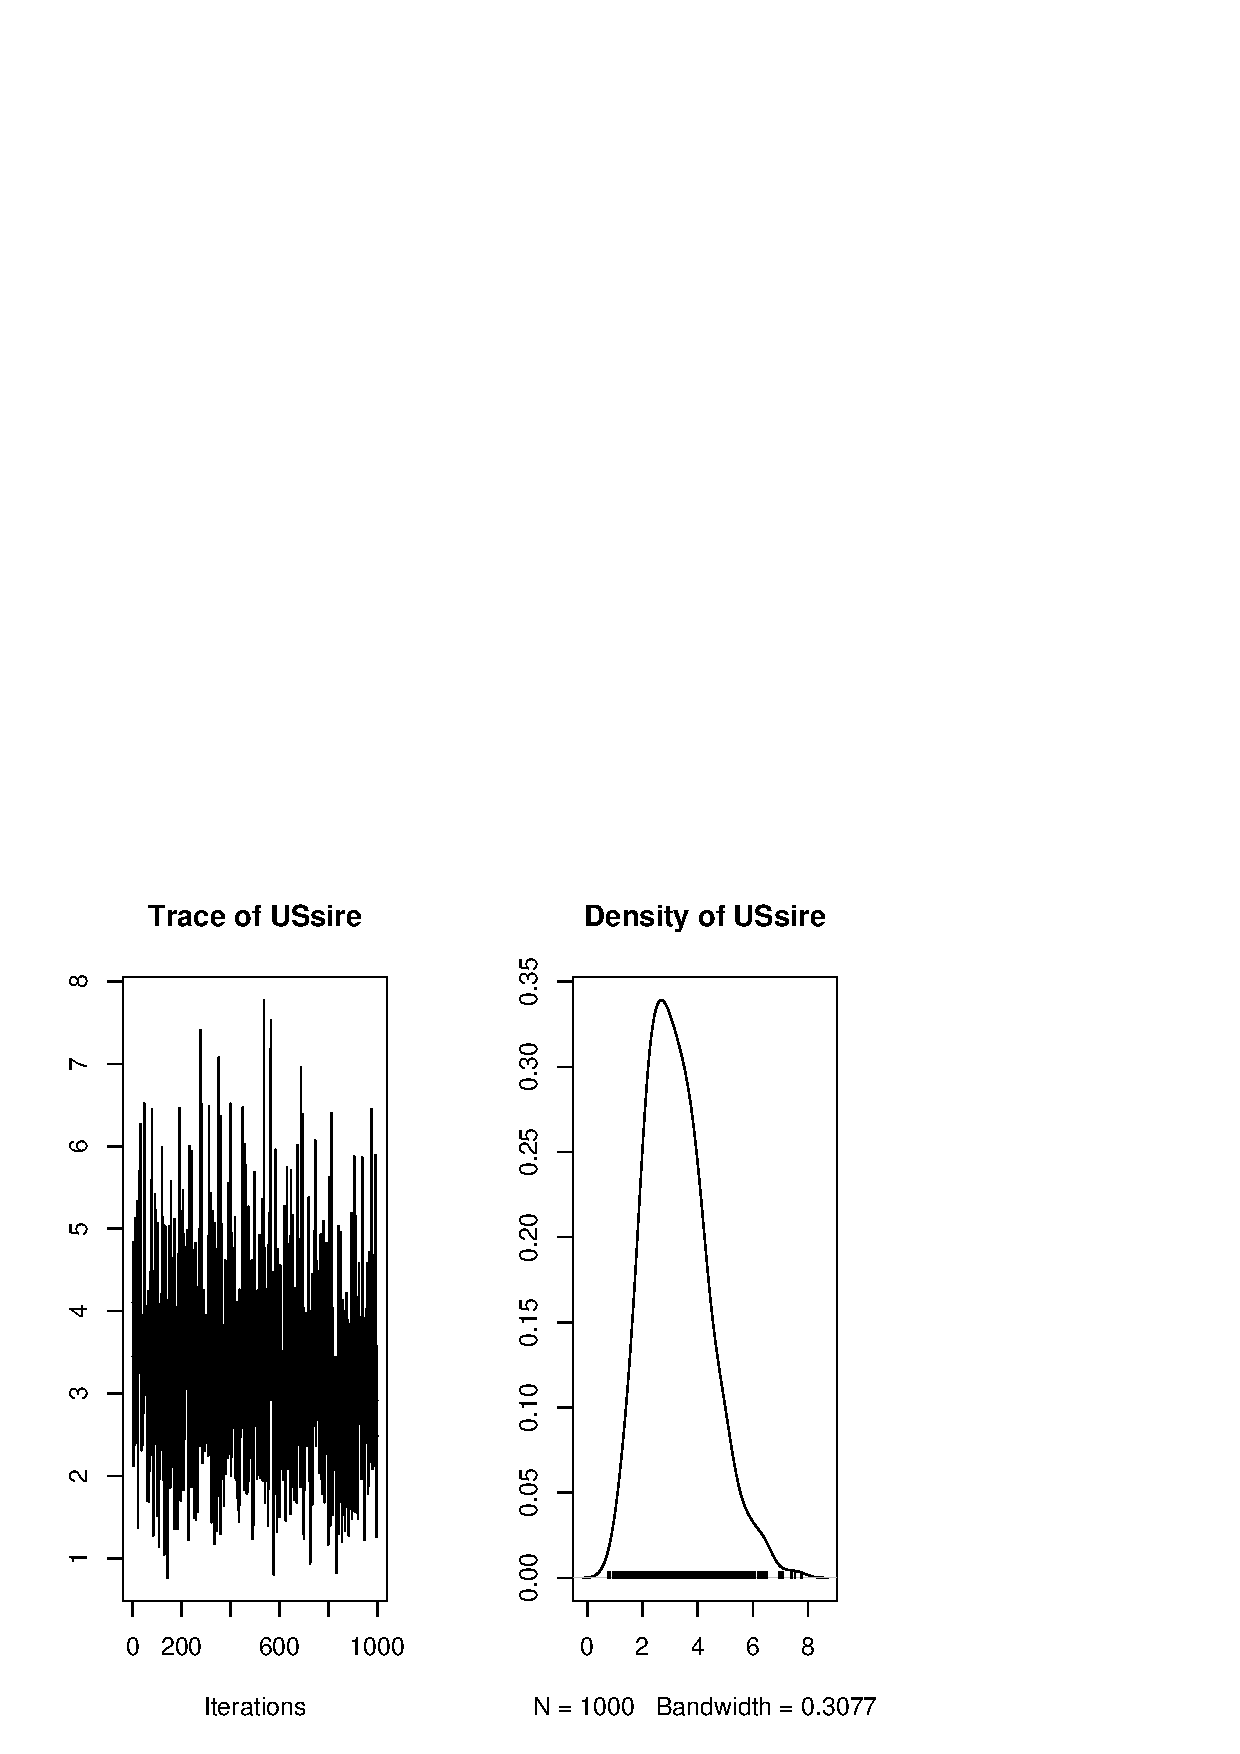
\includegraphics{Tutorial-070}
\end{center}
\caption{The marginal posterior distribution of the number of unsampled males from \texttt{model.miss}, when the pedigree is sampled assuming that the phenotypes of unsampled males are unknown. The actual number is 25!}
\label{EPP1US-fig}
\end{figure}

When \texttt{USvar=NULL}, the records of unsampled fathers do not enter into the likelihood equation for $\beta$, and so $\beta$ is valid.  However, our primary interest was in the within-pair paternity rate, $\beta_{o}$, and we can use equation \ref{eq_thetao} to obtain the posterior

\begin{Schunk}
\begin{Sinput}
> theta <- inv.logit(model.miss$beta)
> NW <- 1
> NE <- 24
> theta_o <- (NW * theta)/(NW * theta + NE * (1 - theta))
> plot(mcmc(theta_o))
\end{Sinput}
\end{Schunk}


\begin{figure}[!h]
\begin{center}
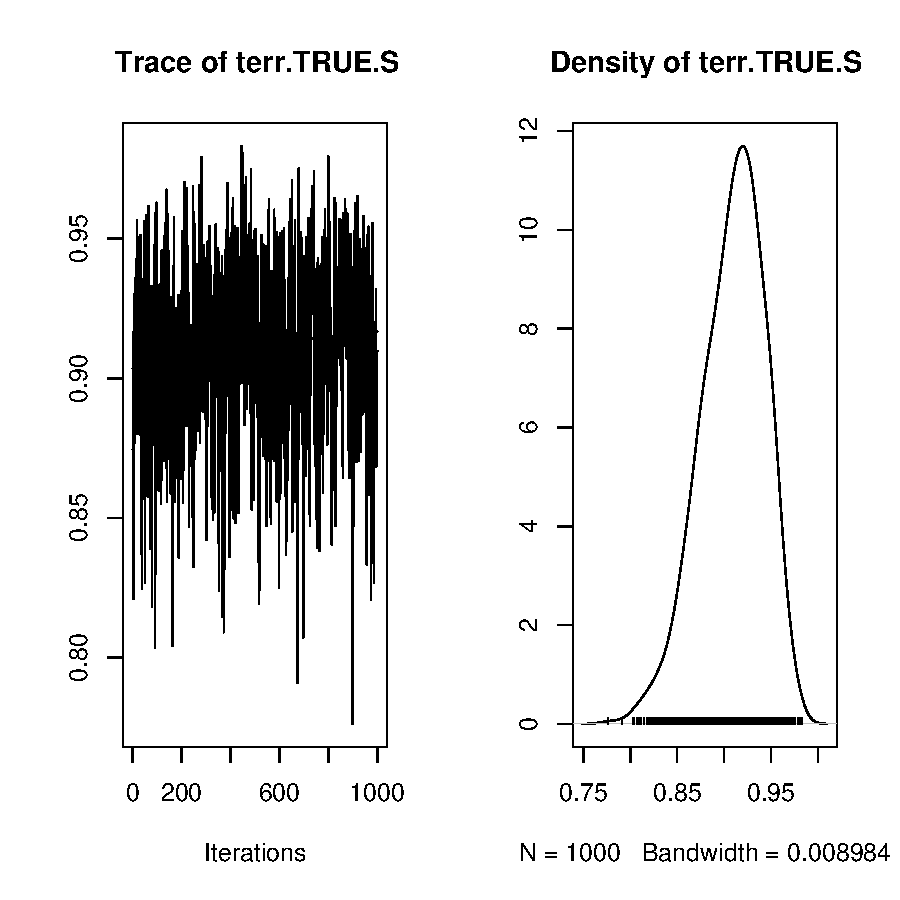
\includegraphics{Tutorial-073}
\end{center}
\caption{The marginal posterior distribution of $\beta_{o}$ derived from \texttt{model.miss}.  $\beta_{o}$ should be the level of within pair paternity in the population (80\%) but we can see that this value has a small posterior probability.  This may be down to sampling error alone, but in fact the estimate is consistently biased upwards because the pedigree is sampled assuming that the phenotypes of unsampled males are unknown.}
\label{EPP1Test-fig}
\end{figure}


Given the mode of the posterior of $\beta$ is very close to 5.28 (Figure \ref{EPP1-fig}), it seems surprising that the mode of the within-pair paternity rate is not 0.8 (Figure \ref{EPP1Test-fig}). We can go one step better and specify that the phenotypes of the unsampled males are known 

\begin{Schunk}
\begin{Sinput}
> var2 <- expression(varPed(x = "terr", gender = "Male", relational = "OFFSPRING", 
+     USvar = FALSE))
> PdP_miss2 <- PdataPed(formula = list(res1, var2, res2), data = data_EPP_miss, 
+     USsire = TRUE)
> model.miss2 <- MCMCped(PdP = PdP_miss2, GdP = GdP_miss, verbose = FALSE)
> plot(model.miss2$beta)
> plot(model.miss2$USsire)
\end{Sinput}
\end{Schunk}


\begin{figure}[!h]
\begin{center}
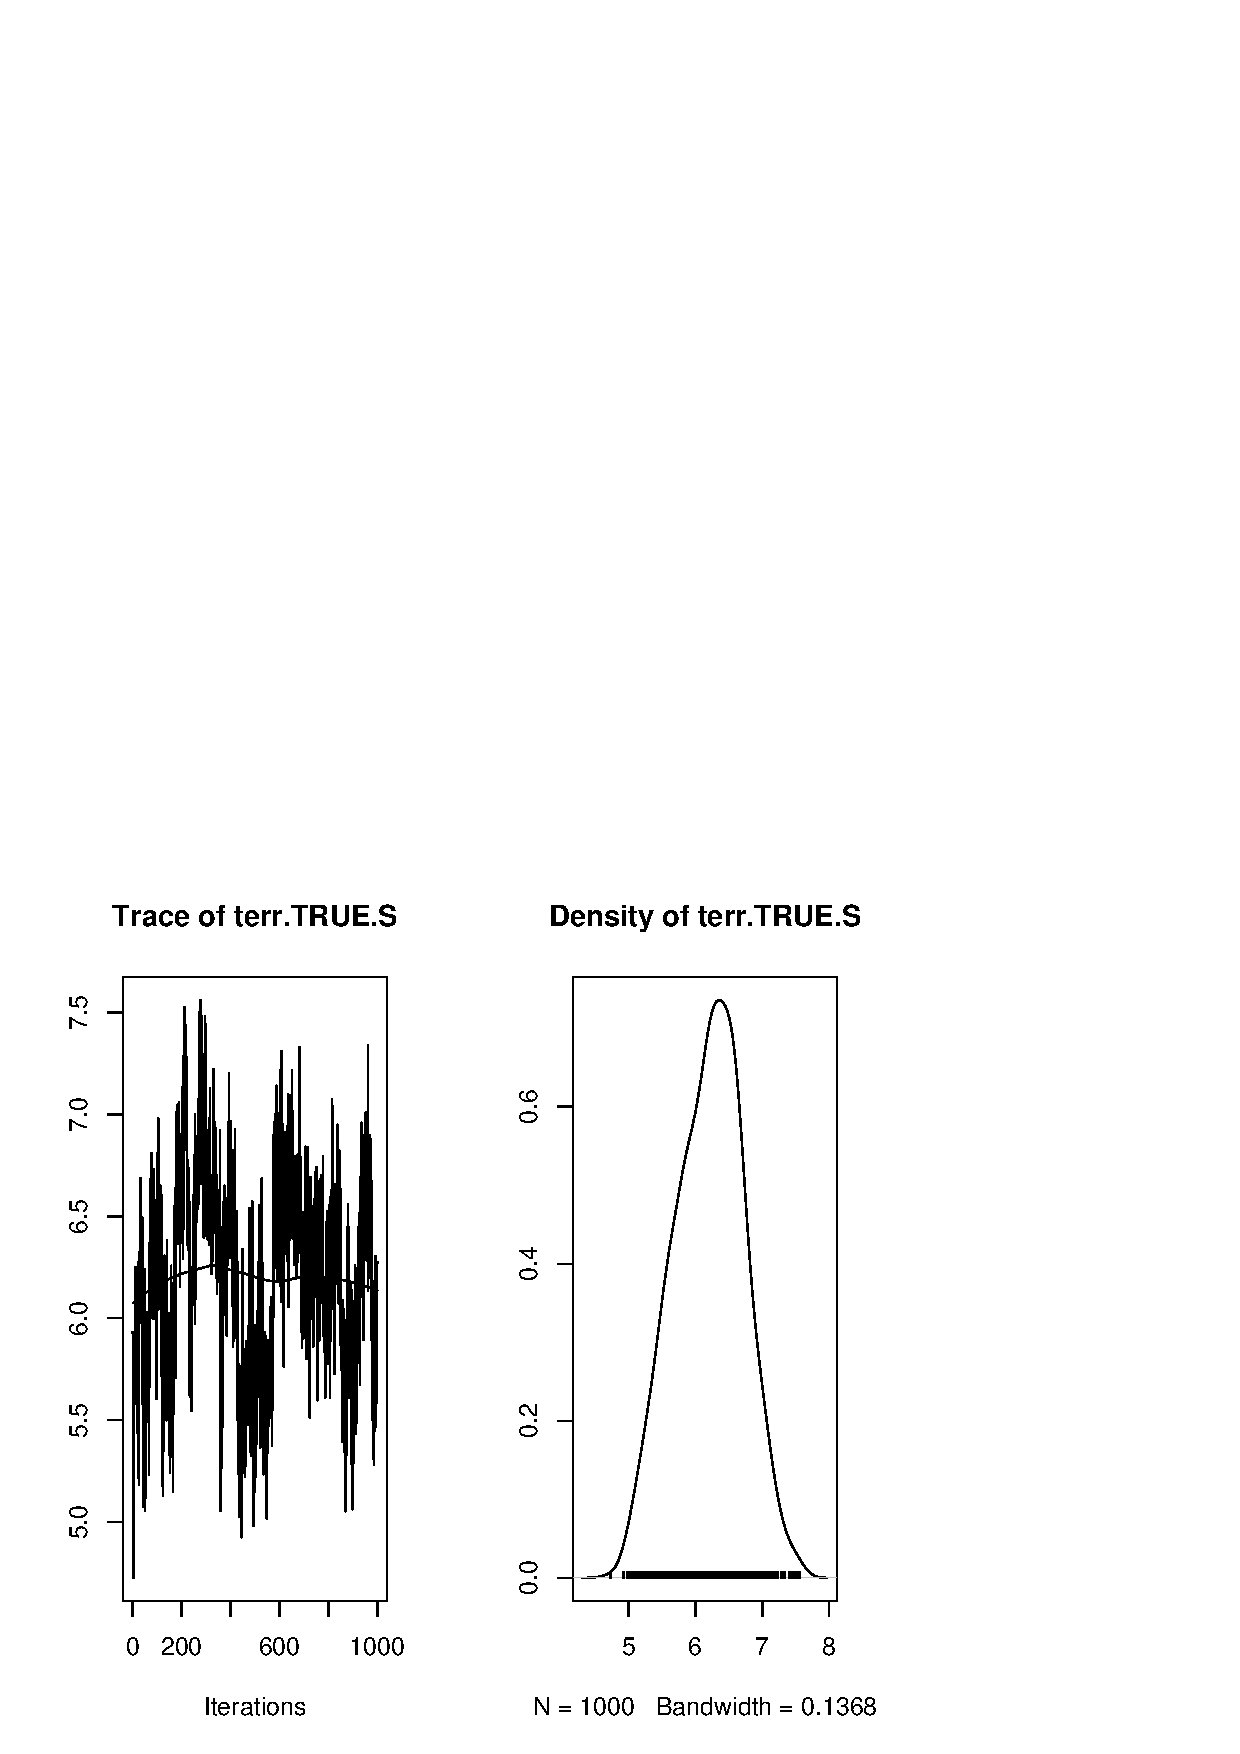
\includegraphics{Tutorial-076}
\end{center}
\caption{The marginal posterior distribution of $\beta$ derived from \texttt{model.miss2}. As in Figure \ref{EPP1-fig} this is the log odds ratio of a male scoring paternity if it had been on the offspring's territory compared to if it had been on a different territory. However, in this model the pedigree is sampled assuming that the unsampled males have to be extra-pair, and these males contribute to the likelihood of $\beta$.}
\label{model.miss2-fig}
\end{figure}

Once again $\beta$ is estimated correctly (Figure \ref{model.miss2-fig}), but this time the number of unsampled males is estimated correctly, although considerable uncertainty remains (Figure \ref{model.miss2US-fig}).  In part this is due to the moderate levels of genotyping error.\\


\begin{figure}[!h]
\begin{center}
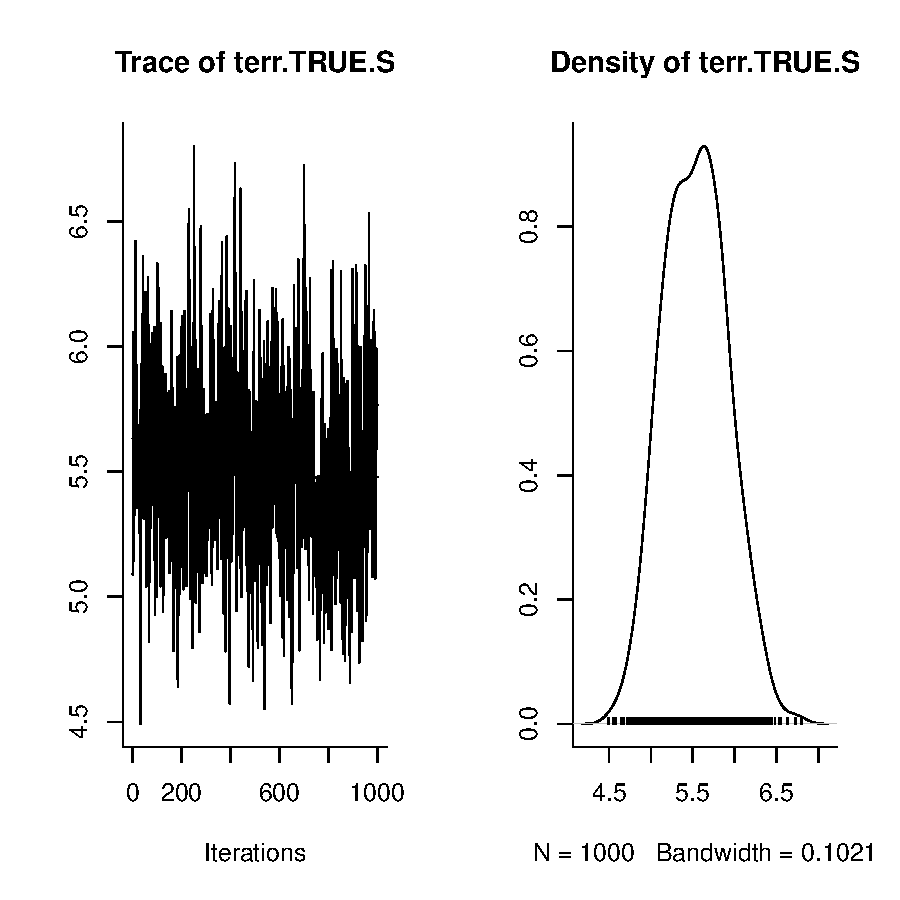
\includegraphics{Tutorial-078}
\end{center}
\caption{The marginal posterior distribution of the number of unsampled males from \texttt{model.miss2}.  The true number is 25.}
\label{model.miss2US-fig}
\end{figure}

We can derive the posterior distribution for within-pair paternity by combining the posterior distribution of $\beta$ with the number of unsampled males, which we have assumed are extra-territorial males.

\begin{Schunk}
\begin{Sinput}
> theta <- inv.logit(model.miss2$beta)
> NW <- 1
> NE <- 24 + model.miss2$USsire
> theta_o <- (NW * theta)/(NW * theta + NE * (1 - theta))
> plot(mcmc(theta_o))
\end{Sinput}
\end{Schunk}


\begin{figure}[!h]
\begin{center}
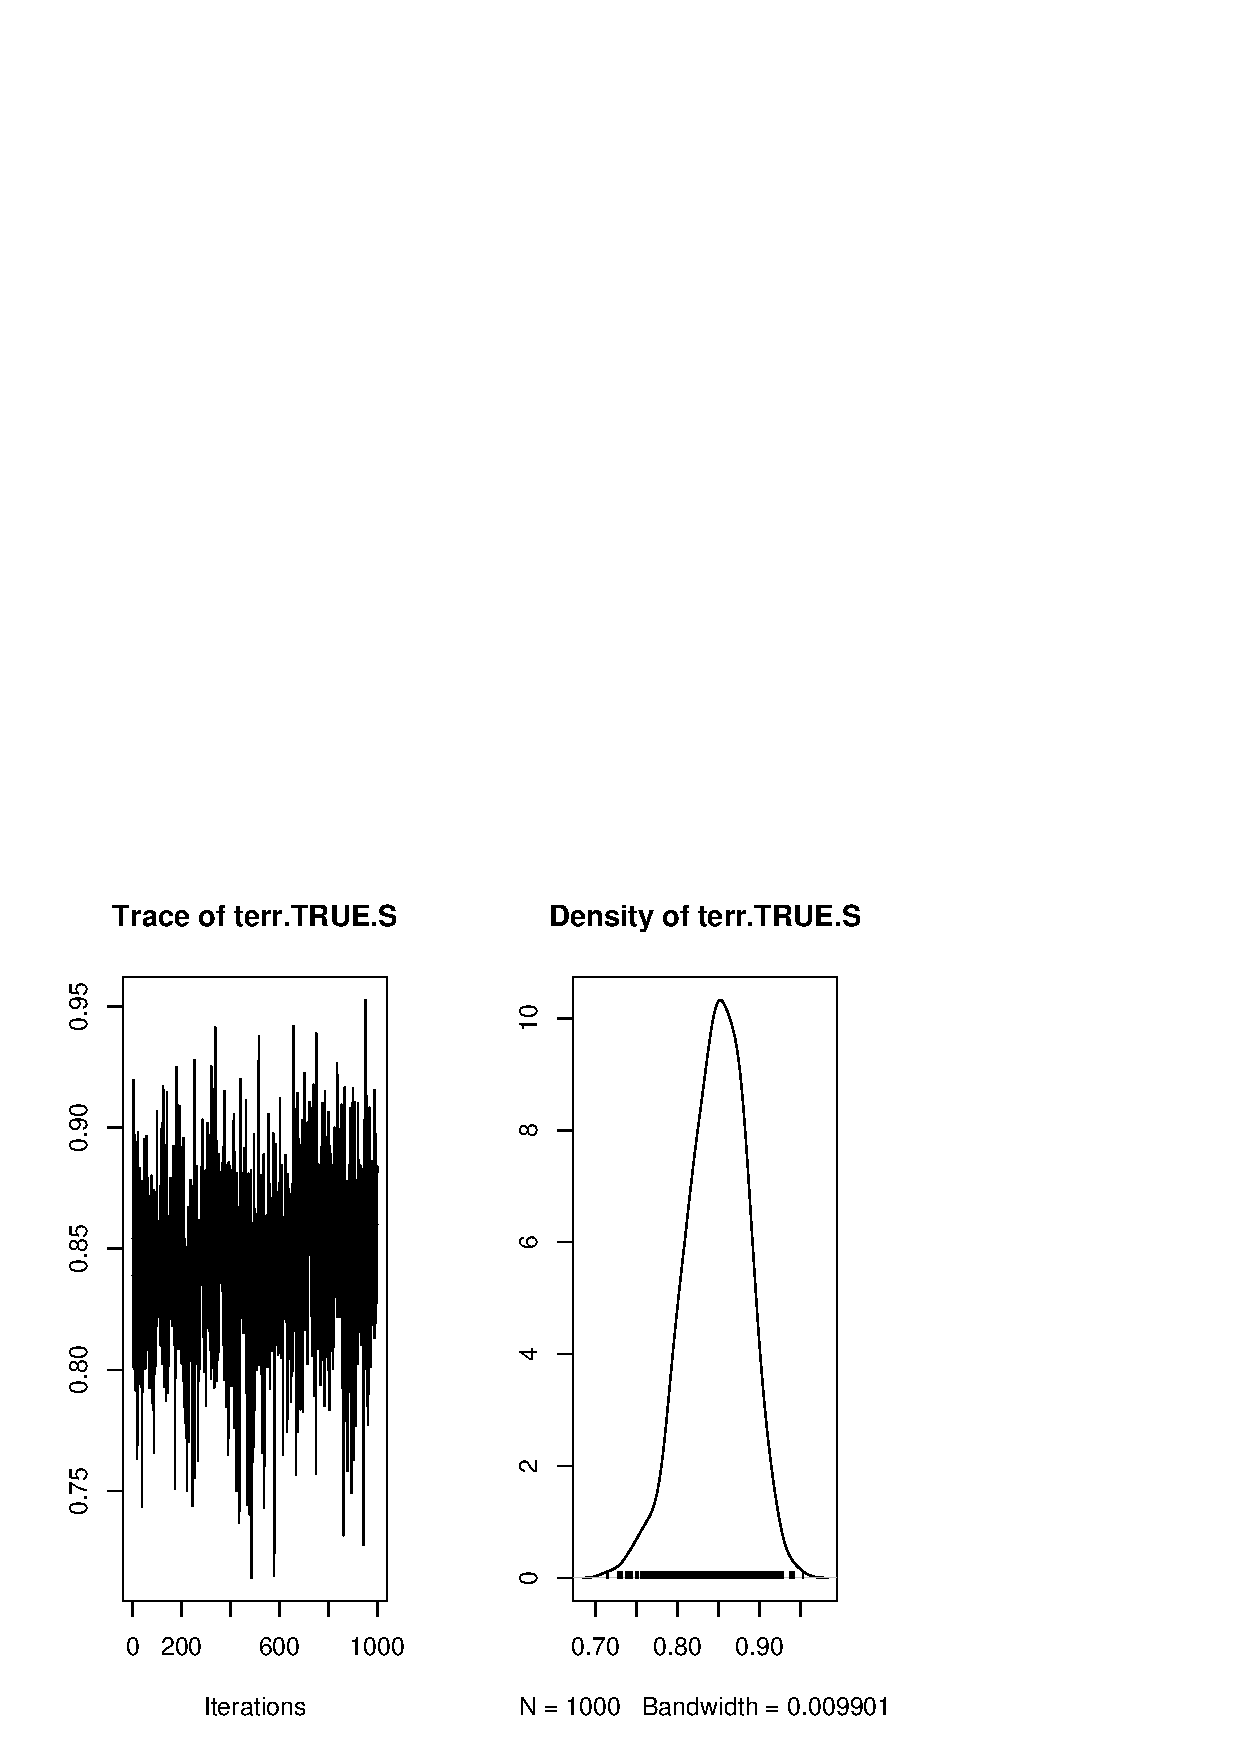
\includegraphics{Tutorial-081}
\end{center}
\caption{The marginal posterior distribution of within-pair paternity estimated from the posterior distributions of $\beta$ and the number of unsampled males from \texttt{model.miss2}.}
\label{EPP2Test-fig}
\end{figure}

The estimate of within-pair paternity from \texttt{model.miss2} is plotted in Figure \ref{EPP2Test-fig}.  Alternativley we can fit within-pair paternity explicitly using the argument \texttt{merge}. 

\begin{Schunk}
\begin{Sinput}
> var3 <- expression(varPed(x = "terr", gender = "Male", relational = "OFFSPRING", 
+     USvar = FALSE, merge = TRUE))
> PdP_miss3 <- PdataPed(formula = list(res1, var3, res2), data = data_EPP_miss, 
+     USsire = TRUE)
> model.miss3 <- MCMCped(PdP = PdP_miss3, GdP = GdP_miss, verbose = FALSE)
> theta_o <- inv.logit(model.miss3$beta)
> plot(mcmc(theta_o))
\end{Sinput}
\end{Schunk}


\begin{figure}[!h]
\begin{center}
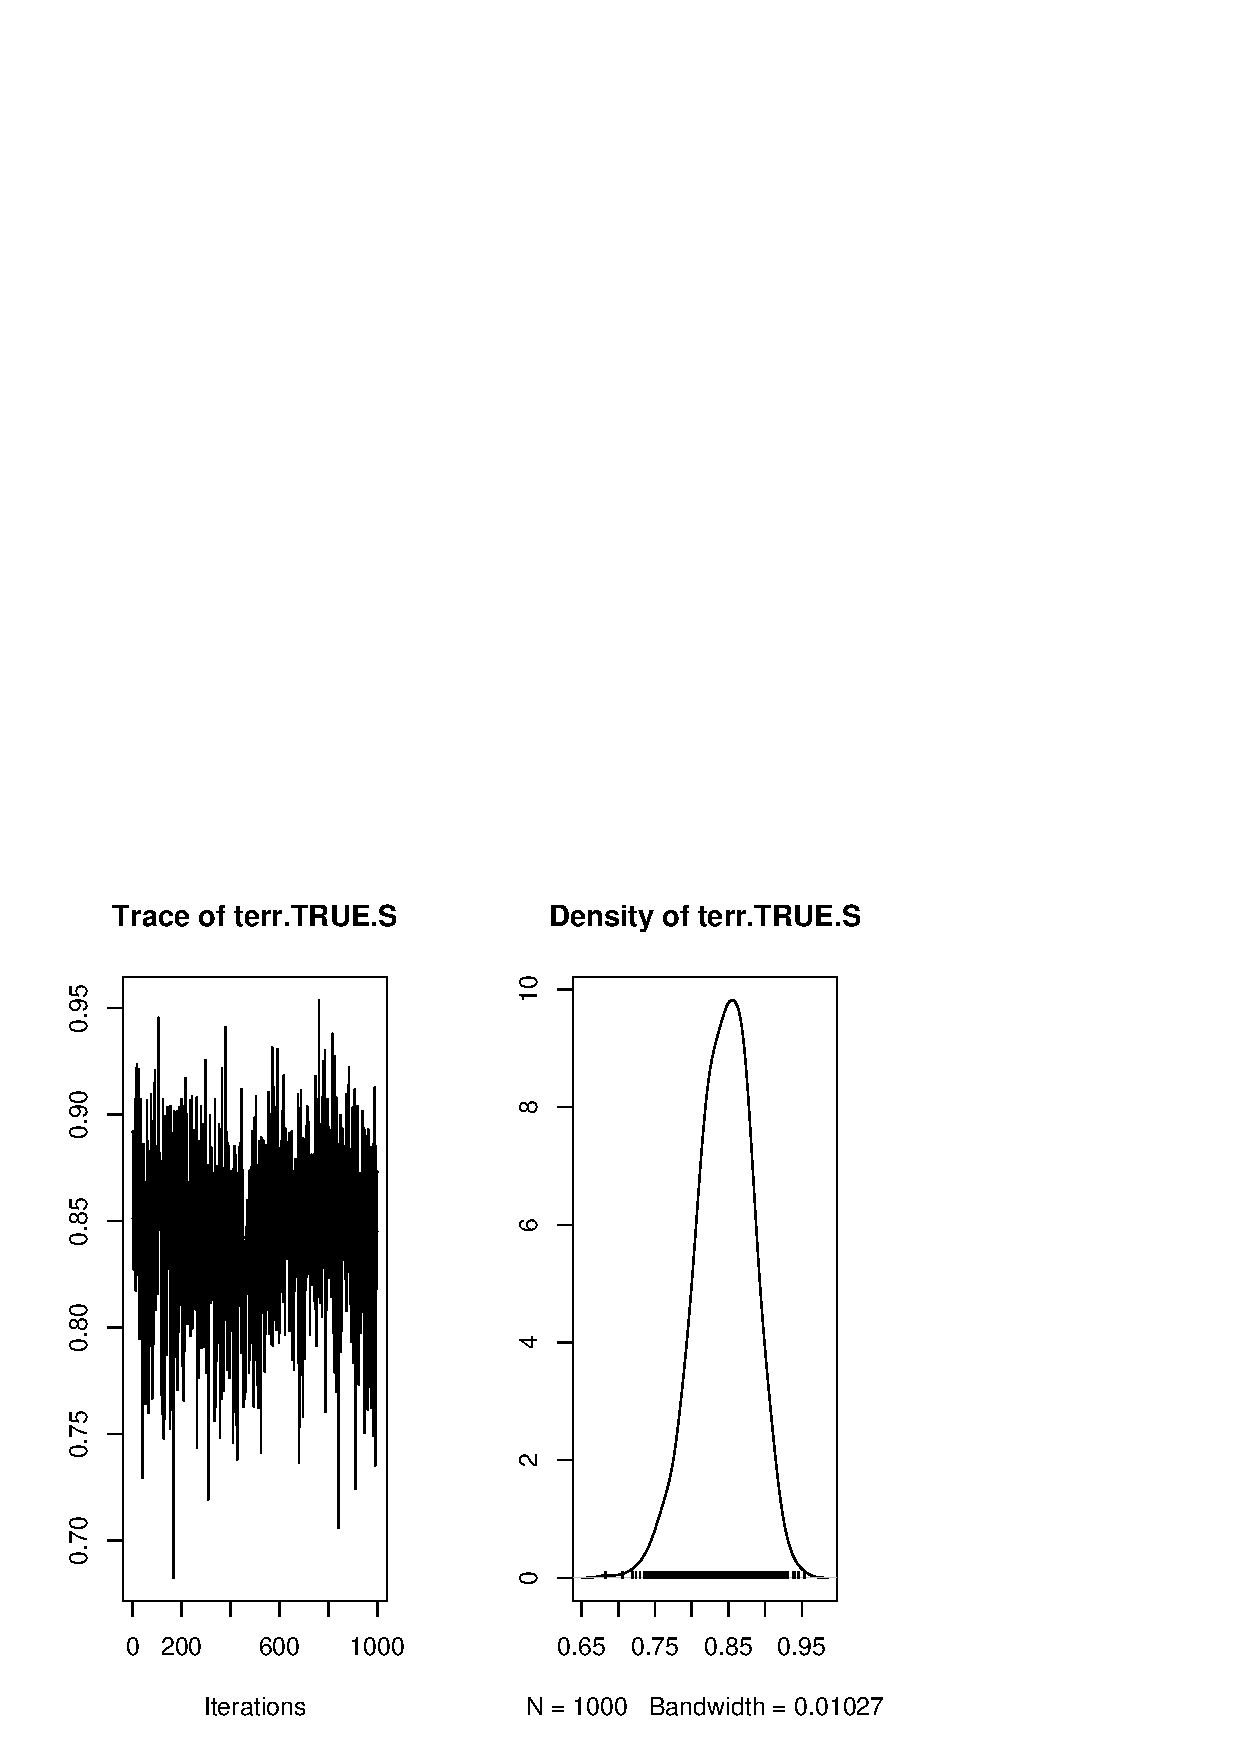
\includegraphics{Tutorial-084}
\end{center}
\caption{The marginal posterior distribution of within-pair paternity estimated directly in \texttt{model.miss3}. The posterior distribution is exactly equivalent to that shown in Figure \ref{EPP2Test-fig}.}
\label{EPPmerge-fig}
\end{figure}


In this example the estimate of within-pair paternity in \texttt{model.miss2} (Figure \ref{EPP2Test-fig}) and \texttt{model.miss3} (Figure \ref{EPPmerge-fig}) are equivalent, but for analyses where the set of males varies between offspring the two models would not be equivalent.  For example, if the aim was to model a constant extra-pair paternity rate across years but the male population size fluctuated between years then the argument \texttt{merge=TRUE} would have to be specified.  In this instance, a \emph{post-hoc} transformation of $\beta$ and the number of unsampled males would not yield a valid posterior for $\beta_{o}$ as it did in the simple example above (Figure \ref{EPP2Test-fig}).   

\subsection{Assortative Mating and Heritability}

Assortative and disassortative mating can modelled using the argument \texttt{relational="MATE"} in \texttt{varPed}. This sets up a variable for the distance between male and female phenotypes.  If the variable is numeric then this distance is Euclidean, if the variable is categorical then the distance is simply one or zero, depending on whether the sexes belong to the same category or not.  Below we will consider a population of 10 males, 10 females, and 30 offspring.  There are 2 mating types, + and -, and they are distributed evenly across and within the sexes.   The aim is to test whether unions such +/+ and -/- occur more often than +/- unions, than would be expected by chance.  We will simulate data where assortative unions are 3 times more likely than disassortative unions than would be expected under random mating.  

\begin{equation}
p^{(o)}_{i,j} \propto \textrm{exp}(\beta_{1}\delta_{i,j})
\label{AM-eq}
\end{equation}

$\delta_{i,j}$ takes on the value one when the mating type of female $i$ matches the mating type of male $j$, and $\beta_{1}$ in this example is log(3).

\begin{Schunk}
\begin{Sinput}
> id <- 1:50
> sex <- rep(c("Male", "Female"), each = 10, length = 50)
> offspring <- c(rep(0, 20), rep(1, 30))
> MT <- gl(2, 1, 50, labels = c("+", "-"))
> test.data <- data.frame(id, offspring, MT, sex)
> res1 <- expression(varPed("offspring", restrict = 0))
> var2 <- expression(varPed(c("MT"), gender = "Female", relational = "MATE"))
> PdP <- PdataPed(formula = list(res1, var2), data = test.data)
> simped <- simpedigree(PdP, beta = logit(0.75))
> table(MT[as.numeric(simped$ped[, 2])] == MT[as.numeric(simped$ped[, 
+     3])])
\end{Sinput}
\begin{Soutput}
FALSE  TRUE 
    9    21 
\end{Soutput}
\begin{Sinput}
> G <- simgenotypes(A = A, E1 = 0.005, E2 = 0.005, ped = simped$ped, 
+     no_dup = 1)
> GdP <- GdataPed(G = G$Gobs, id = G$id)
> model.ass.mat <- MCMCped(PdP = PdP, GdP = GdP, verbose = FALSE)
> plot(mcmc(inv.logit(model.ass.mat$beta)))
\end{Sinput}
\end{Schunk}


\begin{figure}[!h]
\begin{center}
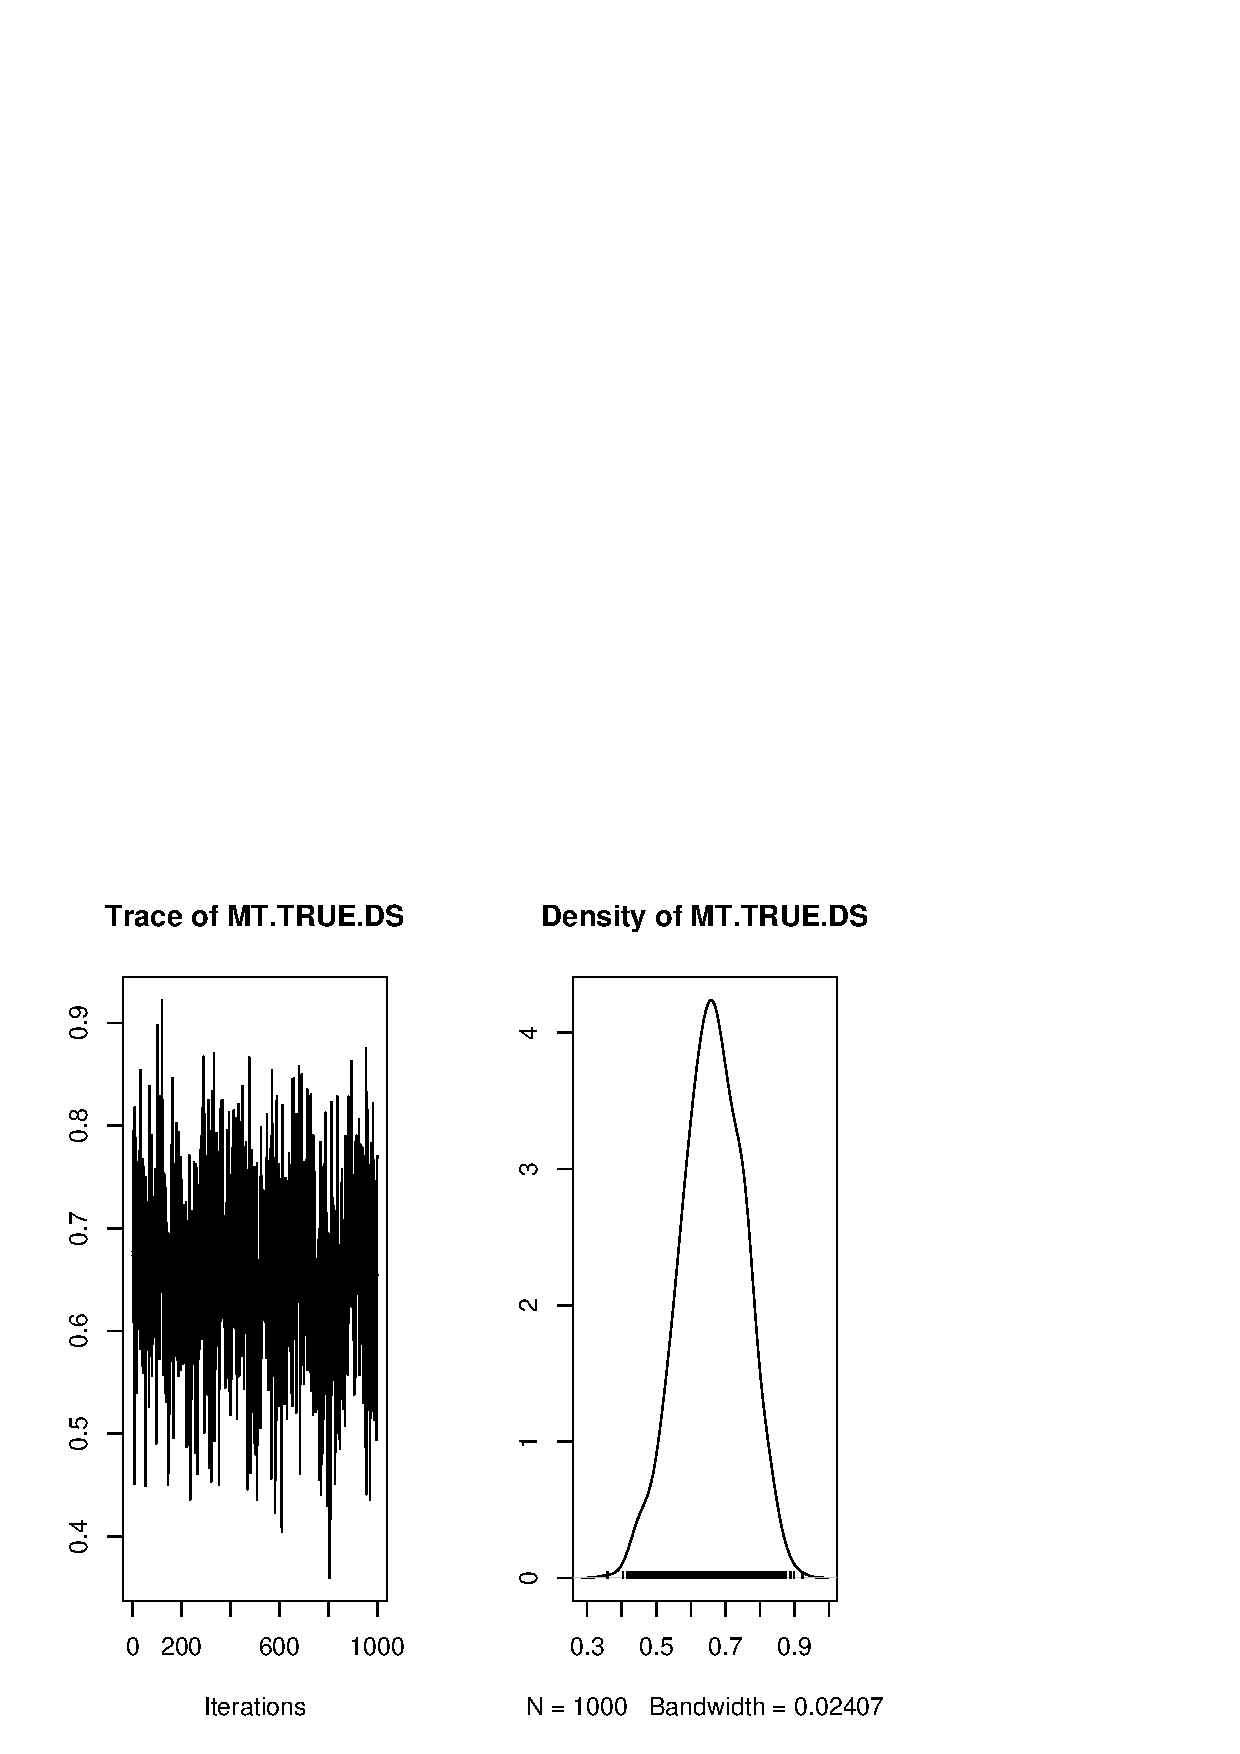
\includegraphics{Tutorial-087}
\end{center}
\caption{The posterior distribution of $\textrm{logit}^{-1}(\beta)$.  In this instance the frequencies of the two mating types are exactly 0.5 both within sexes, and between the sexes, and this is the expected proportion of offspring resulting from the union of +/+ and -/- parents.}
\label{model.ass.mat}
\end{figure}

Mating types may well be inherited, and if we had data on the mating types of offspring we may be inclined to also model the distance between offspring and parental phenotypes using the argument \texttt{relational="OFFSPRING"}.  A cautionary note should be made about using \texttt{relational="OFFSPRING"} to model the transmission of phenotypes between parents and offspring.  If the individuals in the above example were haploid, and mating type was under the control of a single locus then the function \texttt{relational="OFFSPRING"} may capture the genetic process quite well.  On the otherhand, if the organisms were diploid then the model would certainly not be consistent with a genetic process.  Likewise, parameters associated with continuous variables derived using \texttt{relational="OFFSPRING"} should not be interpreted as a measure of heritibility in the quantitative genetic sense, although they will be related.  Future work is planned in this direction.

\subsection{Longitudinal Data and Multigenerational Pedigrees}
\label{pedigree-sec}

MasterBayes is able to work with longitudinal data, allowing the possibility of reconstructing multigenerational pedigrees.  To work with longitudinal data a time variable needs to be passed to \texttt{PdataPed}.  It is VERY important that inidviduals with offspring records do not appear as potential parents of offspring with records in the same cohort, or a previous cohort \footnote{In later versions of MasterBayes ($>2.1$) the argument \texttt{checkP=TRUE} can be passed to \texttt{MCMCped}.  This relaxes the restriction that potential parents do not appear in the set of potential offspring, and so can be used to estimate pedigrees when cohort or age data do not exist.  In such cases the probability that indiviual $i$ is the offspring of individual $j$ may have a similar posterior probability to the reverse scenario where indiviual $j$ is the offspring of individual $i$.  The new function \texttt{post.pairs} will calculate posterior probabilities for 2 indiviuals falling into a certain relationship (e.g. parent-offspring or offspring-parent) when the joint posterior distribution of pedigrees are stored (i.e. \texttt{write\_postP="TRUE"} is passed to \texttt{MCMCped}).}   The argument \texttt{restrict} can be passed to \texttt{varPed} to ensure this does not happen. By not doing this you are allowing for the possibility that an individual can be both the parent and an offspring of another.\\  

\begin{Schunk}
\begin{Sinput}
> id <- 1:50
> year <- rep(1:4, each = 50)
> for (yr in 1:3) {
+     id <- c(id, sample(id[year == yr], 25))
+     id <- c(id, max(id) + 1:25)
+ }
> sex <- rep(c("Male", "Female"), max(id))[id]
> off.within.cohort <- c(rep(0, 25), rep(1, 25))
> offspring <- c(rep(0, 50), rep(off.within.cohort, 3))
> lat <- runif(200)
> long <- runif(200)
> data.ped <- data.frame(id, sex, offspring, lat, long, year)
> res1 <- expression(varPed(x = "offspring", restrict = 0))
> res2 <- expression(varPed(x = "year", relational = "OFFSPRING", 
+     restrict = "=="))
> var1 <- expression(varPed(x = c("lat", "long"), lag = c(0, 0), 
+     relational = "OFFSPRING"))
> PdP <- PdataPed(formula = list(res1, res2, var1), data = data.ped, 
+     timevar = year)
> P <- simpedigree(PdP, beta = -1)$ped
> G <- simgenotypes(A = A, ped = P)
> GdP <- GdataPed(G = G$Gobs, id = G$Gid)
> model.ped <- MCMCped(PdP, GdP, mm.tol = 1, verbose = FALSE)
> plot(model.ped$beta)
\end{Sinput}
\end{Schunk}



\begin{figure}[!h]
\begin{center}
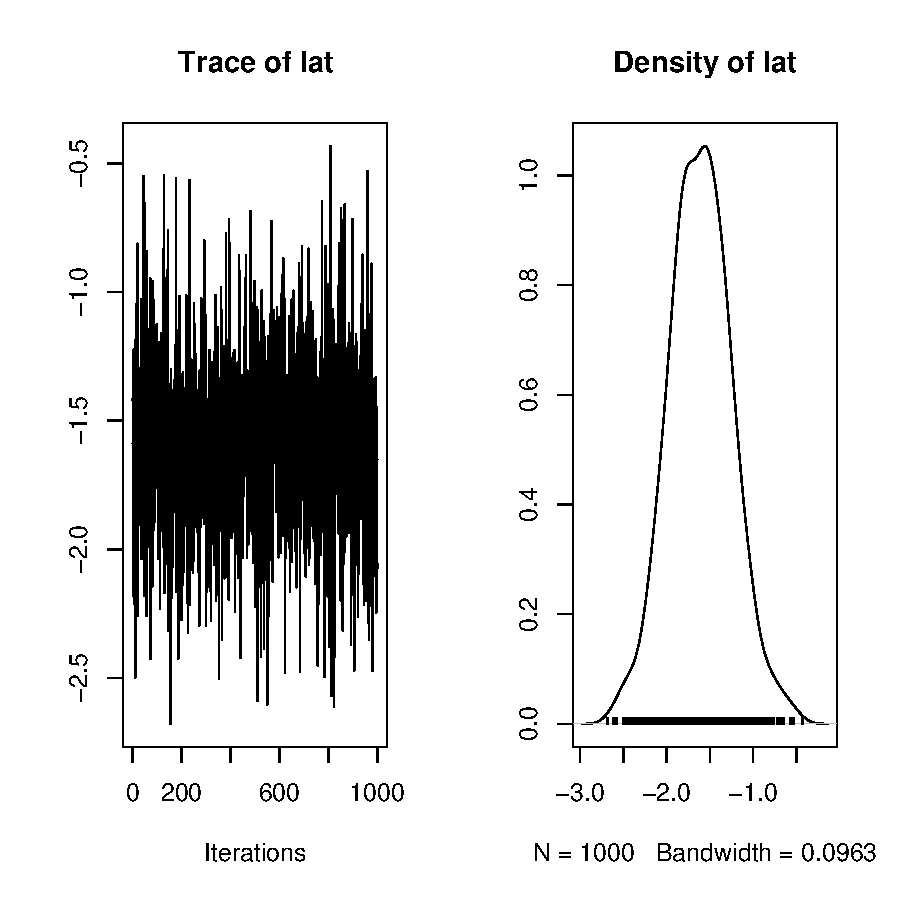
\includegraphics{Tutorial-090}
\end{center}
\caption{The posterior distribution of \texttt{beta}, the rate at which the probability of parentage drops with distance from the offspring.  This parameter was estimated from a multigenerational pedigree where longitudinal data had been collected.  In this toy example, the model was consistent with the data, but for multigenerational problems appropriate models are hard to construct and caution needs to be exercised.}
\label{MGped}
\end{figure}

Several problems currently exist with reconstructing multigenerational pedigrees using MasterBayes.  The first, and perhaps the biggest problem is the assumption that those individuals classed as coming from the base population (including unsampled individuals) are actually unrelated.  For example, if the mother of two sisters (A and B) was not sampled, but sister B was in the set of potential mothers for sister A, then there is a high chance that sister B would be picked as sister A's mother \citep{Thompson.1976a}.  Modelling the possibility that sampled individuals may be related through unsampled individuals is a challenging problem with a long history. In the future I may incorporate the reversible jump MCMC methods outlined in \citet{Emery.2001} to try and alleviate the problem that full-siblings without sampled parents cause.  A second problem with the reconstruction of multigenerational pedigrees, which has recieved much less attention is the problem of inbreeding avoidance.  The likelihood of a genotype configuration given a pedigree can be calculated using the Elston-Stewart algorithm \citep{Elston.1971}, which is based on the product of the Mendelian transition probabilities across offspring.  Most parentage and sib analyses are special cases or approximations of this algorithm.  However, a pedigree has both marriages and births, and an implicit assumption when calculating the likelihood of genotypes given a pedigree is that marriages are independent of genotype. When inbreeding avoidance, or selfing is practised, this assumption breaks down, and could compromise pedigree reconstruction. 

\subsection{Hermaphrodites and Selfing Rates}
\label{Herm-sec}

An extreme form of inbreeding is selfing in hermaphrodites.  MasterBayes is able to work with hermaphrodite systems by not passing a \texttt{sex} vector to \texttt{PdataPed}.  Currently, MasterBayes can be forced to model selfing in hermaphrodites although it is inefficent (the following example took 5 minutes depsite a mismatch tolerance of 1).  More efficient methods will be developed in the future, but a small example will highlight the logic behind the approach, and some of its pitfalls.

\begin{Schunk}
\begin{Sinput}
> id <- as.factor(1:100)
> offspring <- c(rep(0, 25), rep(1, 75))
> Herm <- data.frame(id, offspring)
> res1 <- expression(varPed(x = "offspring", restrict = 0))
> var1 <- expression(varPed(x = "id", relational = "MATE"))
> PdP <- PdataPed(formula = list(res1, var1), data = Herm)
> P <- simpedigree(PdP, beta = logit(0.9))$ped
> G <- simgenotypes(A = A, ped = P)
> GdP <- GdataPed(G = G$Gobs, id = G$Gid)
> model.herm <- MCMCped(PdP, GdP, mm.tol = 1, verbose = FALSE)
> plot(inv.logit(model.herm$beta))
\end{Sinput}
\end{Schunk}


\begin{figure}[!h]
\begin{center}
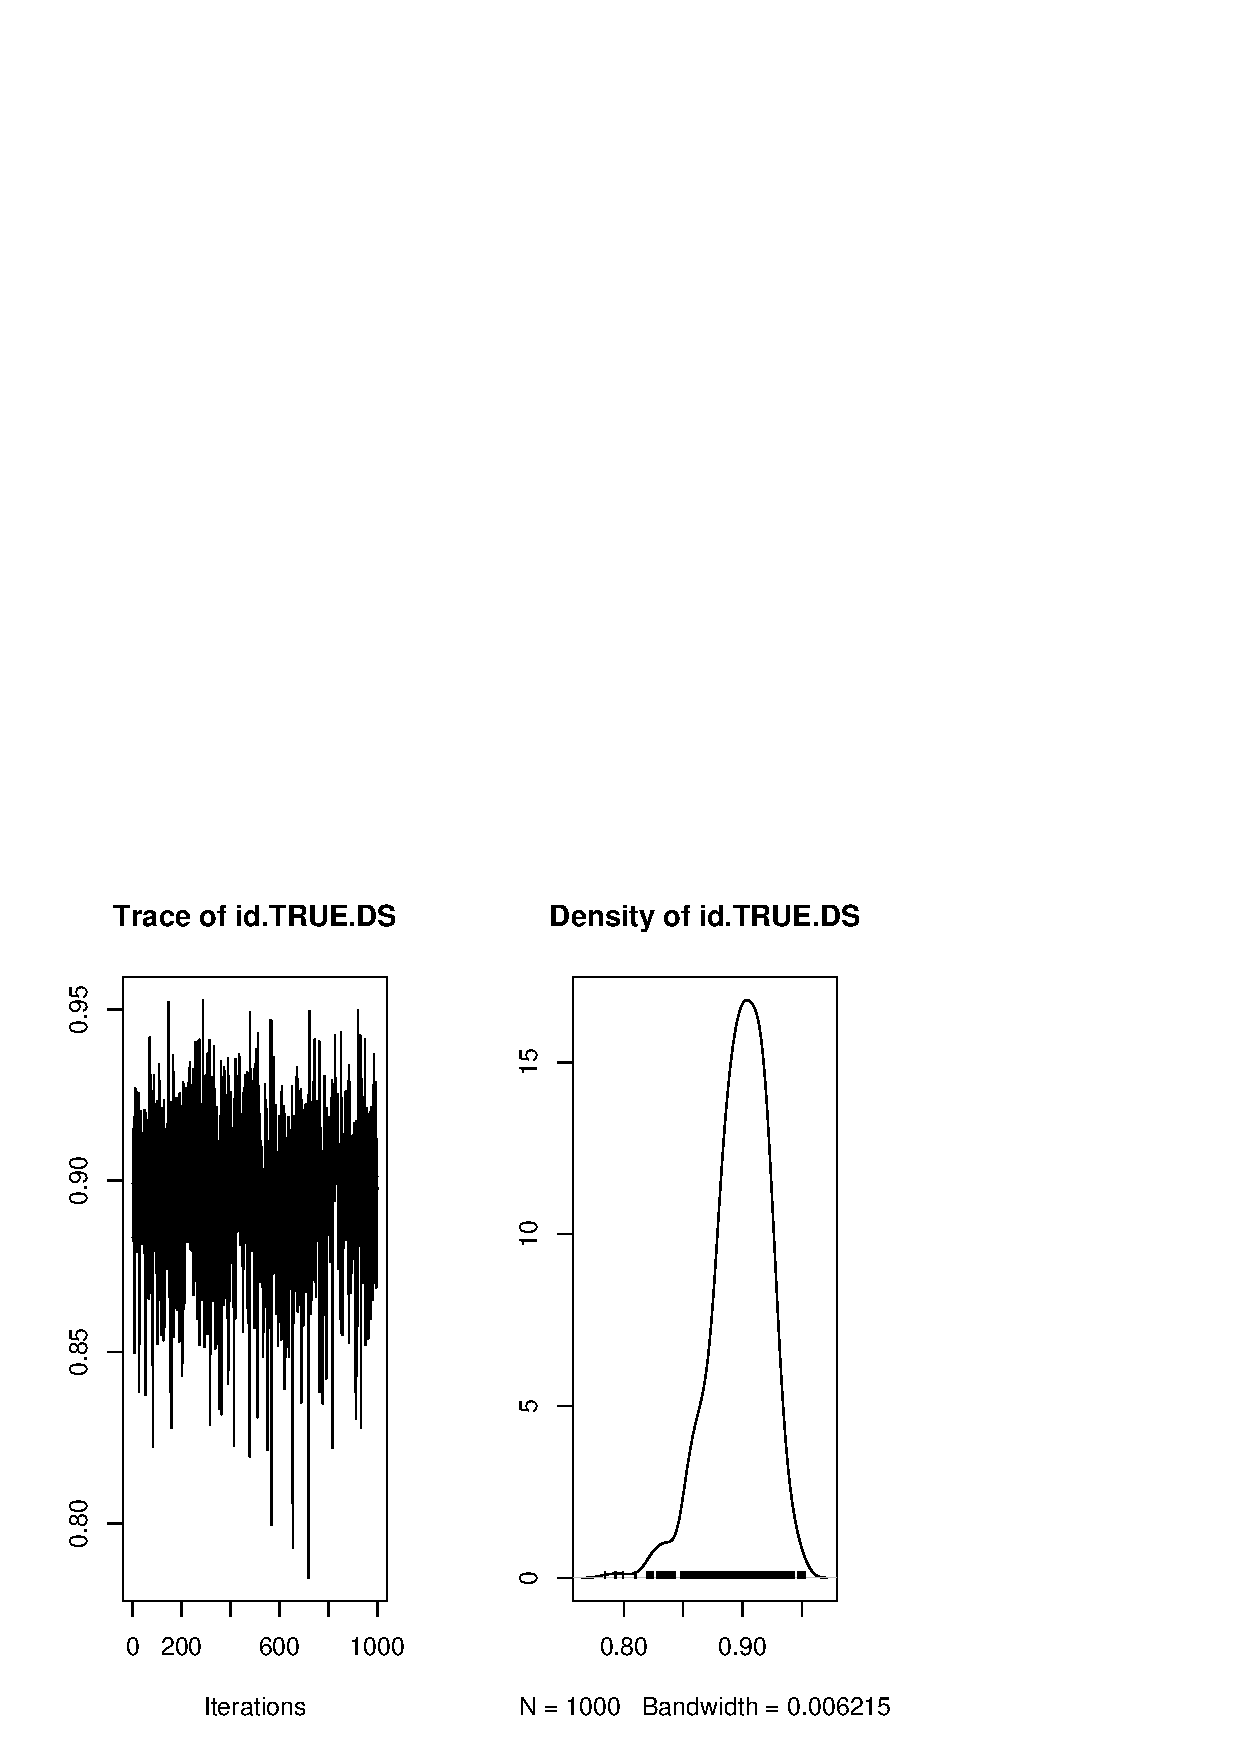
\includegraphics{Tutorial-093}
\end{center}
\caption{The posterior distribution of $\textrm{logit}^{-1}\beta$: the probability that an individual mates with itself compared to another random individual in a hermaphrodite system.}
\label{Herm-fig}
\end{figure}


The model is essentialy one of assortative mating for \texttt{id}, although the genotype updating algorithm becomes a little more complex\footnote{The genotype updating algorithm in earlier versions of MasterBayes (<2.1) had a bug that caused problems when updating the genotypes of individuals that had offspring produced through selfing.}.  \texttt{logit(beta)} should be interpreted as the probability that an individual mates with itself compared to another random individual (Figure \ref{Herm-fig}).  As in Section \ref{EPP-sec}, Equation \ref{eq_thetao} can be used to get the posterior distribution for the expected proportion of offspring produced by selfing.  An important conisderation when the system does not mate randomly is the assumption of Hardy-Weinberg equilibrium.  When evaluating Equation \ref{G_error_p}, genotype frequencies enter into the probability for the true genotypes of base individuals and also those offspring with one or more unsampled parents. These genotype frequencies are calculated from the allele frequencies under the assumption of Hardy-Weinberg equilibrium. For these individuals, the probability distribution of the true genotypes is largely dominated by the observed genotype data rather than the genotype frequencies, and violations of Hardy-Weinberg equilibrium may not be that important.  However, when unsampled parents are present an approximation for the genetic likelihood is used (see Section \ref{us-sec}) that is more reliant on the information imparted by genotype frequencies, and care needs to be taken. 

\subsection{Schrodinger's Hermaphrodite Cat}
\label{SHC}

Monoecy in plants is a common phenomenon; each flower is unisexual but flowers of both sex can be found on the same plant.  The genotype data (unless the fruit or organelles have been typed) provide no information whether an offspring is produced from the male or female flowers of an individual. The only information the genotype data provide is whether the individual is a parent.  However, let's say we measure the proportion of male flowers on the adult plants and this measure positively covaries with pollen production but negatively covaries with seed production.  Alternatively, we could have measured something less sugestive like the distance beween offspring and parents.  MasterBayes can fit gender specific variables to hermaphrodite data but the resulting posteriors are ambiguous with respect to any notion of gender.\\

  To illustrate, we will simulate data from a monoecious population in which the proportion of male flowers on each individual varies substantially. The number of offspring produced by each individual is independent of the proportion of male flowers, but individuals with proportionally more male flowers produce more offspring through pollination.  We will start with a very strong relationship between 'paternity' and the number of male flowers.
 
\begin{Schunk}
\begin{Sinput}
> id <- as.factor(1:100)
> offspring <- c(rep(0, 25), rep(1, 75))
> Prop.male.flowers <- rbeta(100, 10, 10)
> SeedPollen <- data.frame(id, offspring, Prop.male.flowers)
> res1 <- expression(varPed(x = "offspring", restrict = 0))
> var1 <- expression(varPed(x = "Prop.male.flowers", gender = "Male"))
> var2 <- expression(varPed(x = "Prop.male.flowers", gender = "Female"))
> PdP <- PdataPed(formula = list(res1, var1, var2), data = SeedPollen)
> P <- simpedigree(PdP, beta = c(-7.5, 7.5))$ped
> G <- simgenotypes(A = A, ped = P)
> GdP <- GdataPed(G = G$Gobs, id = G$Gid)
> model.mon <- MCMCped(PdP, GdP, mm.tol = 1, verbose = FALSE)
> plot(model.mon$beta)
\end{Sinput}
\end{Schunk}


\begin{figure}[!h]
\begin{center}
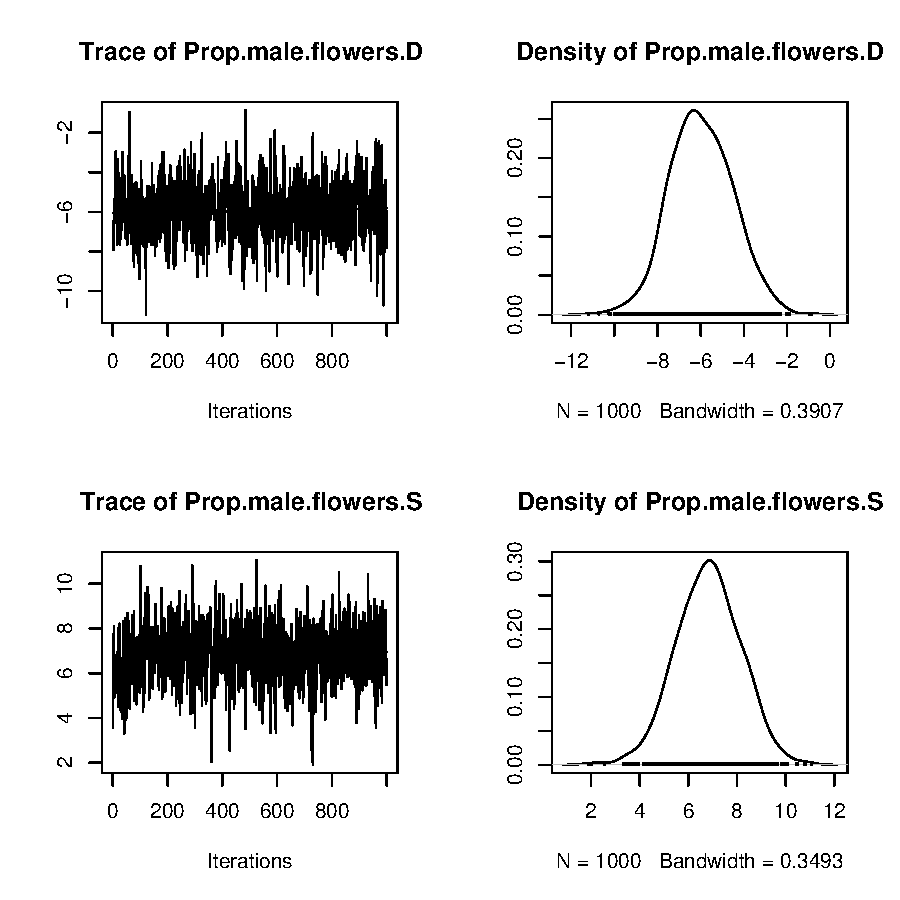
\includegraphics{Tutorial-096}
\end{center}
\caption{The posterior distribution of $\beta$: the parameters of the log-linear relationship between the number of male flowers on a monoecious plant and the probability of producing offspring from female and male flowers, respectively. The relationships are very strong and the chain gets stuck in a region of parameter space of high probability.  A mirror image of this distribution exists outside of the parameter space sampled.}
\label{mon1-fig}
\end{figure}


Figure \ref{mon1-fig} looks reasonable but what happens if we simulate some data where the proportion of male flowers is not such a good predictor of 'paternity/maternity'?  

\begin{Schunk}
\begin{Sinput}
> P <- simpedigree(PdP, beta = c(-4, 4))$ped
> G <- simgenotypes(A = A, ped = P)
> GdP <- GdataPed(G = G$Gobs, id = G$Gid)
> model.mon2 <- MCMCped(PdP, GdP, mm.tol = 1, verbose = FALSE)
> plot(model.mon2$beta)
\end{Sinput}
\end{Schunk}


\begin{figure}[!h]
\begin{center}
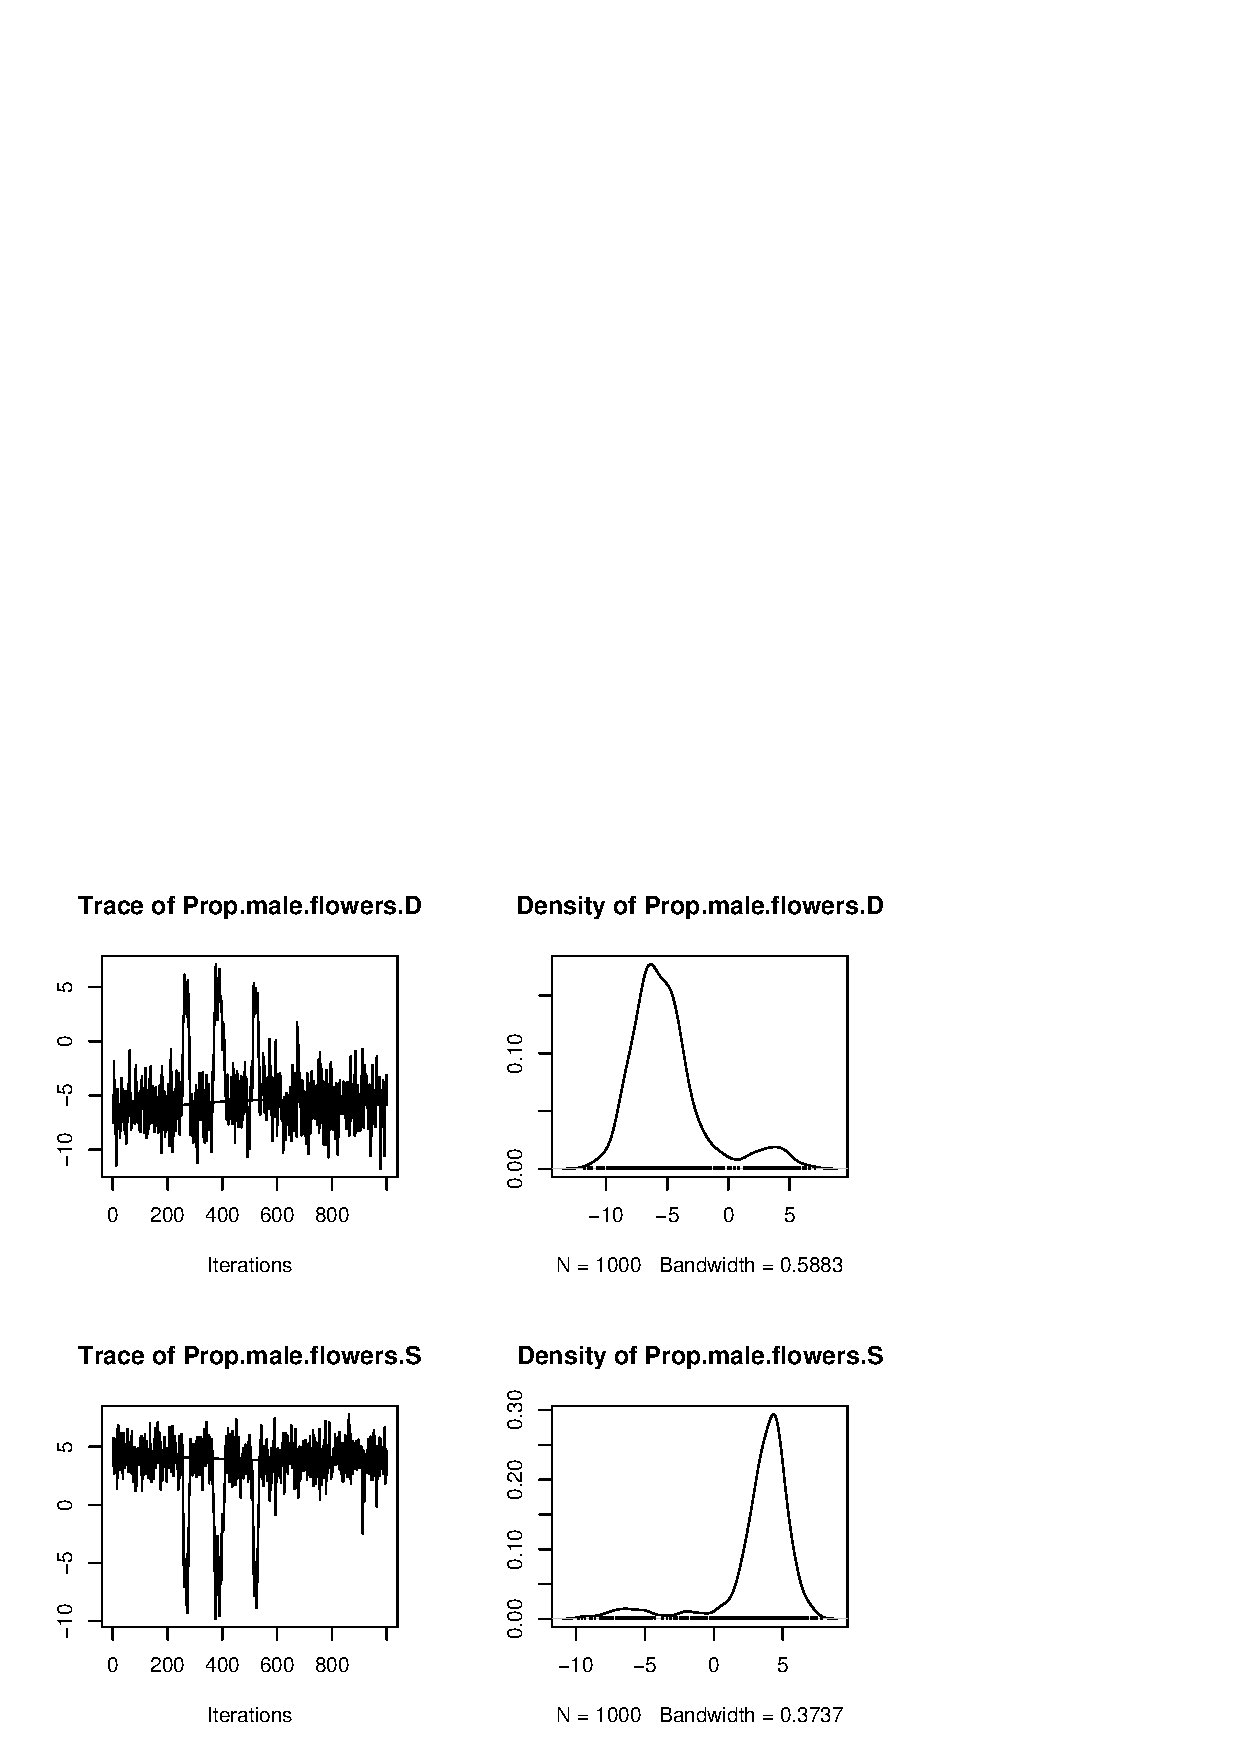
\includegraphics{Tutorial-099}
\end{center}
\caption{The posterior distribution of $\beta$: the parameters of the log-linear relationship between the number of male flowers on a monoecious plant and the probability of producing offspring from female and male flowers, respectively. The relationships are not so strong as in Figure \ref{mon1-fig}, and the chain is able to sample from the full posterior, albeit with a lot of autocorrelation.}
\label{mon2-fig}
\end{figure}

We see that the posterior distribution is actually bimodal (Figure \ref{mon2-fig})! We can be fairly confident that the proportion of male flowers indicates the probability of polination versus seed production, but we have no way of saying what the sign of the relationship is: whether the proportion of male flowers is positively correlated with pollination and negatively correlated with seed production or \emph{vica versa}.  We could probably make an informed guess, but with more amiguous varables it may not be possible to do so.  If any one has any idea on how to set up a sensible prior for this type of model, please email me.  

\newpage
\appendix
\section{A Lightning Tour of Model Specification}
\label{models-app}

$p^{(o)}_{i,j}$ is the probability that female $i$ and male $j$ are the parents of offspring $o$. \texttt{x} are explanatory variable(s), and $\beta$ the vector of associated parameter(s). $t$ indicates the time (\texttt{timevar} in a \texttt{PdataPed} object) to which the offspring record belongs.  For continous variables...

\texttt{varPed(x, gender="Female")}

\begin{equation}
p^{(o)}_{i,j} \propto \textrm{exp}(\beta_{1}\textrm{\texttt{x}}_{i}...)
\end{equation}

\texttt{varPed(x, gender="Male")}

\begin{equation}
p^{(o)}_{i,j} \propto \textrm{exp}(\beta_{1}\textrm{\texttt{x}}_{j}...)
\end{equation}

\texttt{varPed(x)}

\begin{equation}
p^{(o)}_{i,j} \propto \textrm{exp}(\beta_{1}(\textrm{\texttt{x}}_{i}+\textrm{\texttt{x}}_{j})...)
\end{equation}

\texttt{varPed(x, gender="Female", relational="OFFSPRING")}

\begin{equation}
p^{(o)}_{i,j} \propto \textrm{exp}(\beta_{1}(|\textrm{\texttt{x}}_{i}-\textrm{\texttt{x}}_{o}|)...)
\end{equation}

\texttt{varPed(x, gender="Female", relational="OFFSPRINGV")}

\begin{equation}
p^{(o)}_{i,j} \propto \textrm{exp}(\beta_{1}(\textrm{\texttt{x}}_{i}-\textrm{\texttt{x}}_{o})...)
\end{equation}

\texttt{varPed(x, gender="Female", relational="MATE")}

\begin{equation}
p^{(o)}_{i,j} \propto \textrm{exp}(\beta_{1}(|\textrm{\texttt{x}}_{i}-\textrm{\texttt{x}}_{j}|)...)
\end{equation}

\texttt{varPed(x, gender="Female", relational="MATEV")}

\begin{equation}
p^{(o)}_{i,j} \propto \textrm{exp}(\beta_{1}(\textrm{\texttt{x}}_{i}-\textrm{\texttt{x}}_{j})...)
\end{equation}

\texttt{varPed(x, gender="Female", lag=c(-1,-1))}

\begin{equation}
p^{(o)}_{i,j} \propto \textrm{exp}(\beta_{1}\textrm{\texttt{x}}_{i,t-1}...)
\end{equation}

\texttt{varPed(x, gender="Female", lag=c(-1,-1), relational="OFFSPRING")}

\begin{equation}
p^{(o)}_{i,j} \propto \textrm{exp}(\beta_{1}(|\textrm{\texttt{x}}_{i,t-1}-\textrm{\texttt{x}}_{o,t}|)...)
\end{equation}

\texttt{varPed(x, gender="Female", lag=c(0,0), relational="MATE",}\\
\texttt{lag\_relational=c(-1,-1))}

\begin{equation}
p^{(o)}_{i,j} \propto \textrm{exp}(\beta_{1}(|\textrm{\texttt{x}}_{i,t}-\textrm{\texttt{x}}_{j,t-1}|)...)
\end{equation}\\

\texttt{varPed(x, gender="Male", lag=c(0,0), relational="OFFSPRING",}\\
\texttt{lag\_relational=c(-1,-1))}

\begin{equation}
p^{(o)}_{i,j} \propto \textrm{exp}(\beta_{1}(|\textrm{\texttt{x}}_{j,t}-\textrm{\texttt{x}}_{o,t-1}|)...)
\end{equation}\\

For a categorical variable with two levels (\texttt{A} and \texttt{B}) the model specified by \texttt{varPed(x, gender="Female")} takes on the form

\begin{equation}
p^{(o)}_{i,j} \propto \textrm{exp}(\beta_{1}\delta_{i}...)
\end{equation}

where $\delta_{i}$ is an indicator variable taking the value 1 if $\textrm{\texttt{x}}_{i}$ is equal to the first level of \texttt{x} and zero otherwise. $\beta_{1}$ is then the log odds ratio of the two levels of \texttt{x} with respect to maternity.  If \texttt{merge=TRUE} is specified then $\beta_{1}$ may vary across offspring, and $\beta_{o}$ is estimated. $\beta_{o}$ is related to $\beta_{1}$:

\begin{equation}
\beta_{o}  = \textrm{logit}\left[\frac{\theta N_{A}}{\theta N_{A} + (1-\theta)N_{B}}\right]
\end{equation}

where $\theta$ is the inverse logit transformation of $\beta_{1}$, and $N_{A}$ and $N_{B}$ are the number of potential mothers that have level \texttt{A} and \texttt{B} for \texttt{x}. If $N_{A}$ and $N_{B}$ are invariant over offspring the models are functionally equivalent.\\

The denominator of the multinomial likelihood is the summed linear predictors of all possible parents (after setting up a contrast with the baseline parents) \citep{Smouse.1999}.  Designating the first set of parents as baseline, the contrast for each set of parents is simply:

\begin{equation}
\eta^{(o)}_{i,j}  = \textrm{log}\left[\frac{p^{(o)}_{i,j}}{p^{(o)}_{1,1}}\right]
\end{equation}

and the likelihood of $\bm{\beta}$

\begin{equation}
Pr(x|\bm{\beta})  = \prod^{n_{o}}_{o}\left[\frac{\textrm{exp}(\eta^{(o)}_{d,s})}{\sum^{n^{(o)}_{i}}_{i=1}\sum^{n^{(o)}_{j}}_{j=1}\textrm{exp}(\eta^{(o)}_{i,j})}\right] 
\end{equation}

where $n_{o}$, $n^{(o)}_{i}$ and $n^{(o)}_{j}$ are the number of offspring, the number of potential mothers for offspring $o$, and the number of potential fathers for offspring $o$, respectively.  $d$ and $s$ are the actual parents of offspring $o$. The set of possible parents  in the denominator of the multinomial likelihood are those that are not excluded using the argument \texttt{restrict}. However, if the argument \texttt{keep=TRUE} is used then the denominator of the likelihood will include excluded parents depsite the fact that $d \neq i$ and $s \neq j$.

\bibliographystyle{plainnat}

\bibliography{MasterBayes}

\end{document}
 
